% Shared preamble for the CIG-AMF formal-research papers.
% IEEEtran conference class; compiles on Overleaf without modification.
\documentclass[conference]{IEEEtran}
\IEEEoverridecommandlockouts

\usepackage{cite}
\usepackage{amsmath,amssymb,amsfonts}
\usepackage{amsthm}
\usepackage{algorithm}
\usepackage{algorithmic}
\usepackage{graphicx}
\usepackage{textcomp}
\usepackage{xcolor}
\usepackage{booktabs}
\usepackage{url}
\usepackage[hidelinks]{hyperref}

\def\BibTeX{{\rm B\kern-.05em{\sc i\kern-.025em b}\kern-.08em T\kern-.1667em\lower.7ex\hbox{E}\kern-.125emX}}

\newtheorem{theorem}{Theorem}
\newtheorem{lemma}[theorem]{Lemma}
\newtheorem{proposition}[theorem]{Proposition}
\newtheorem{corollary}[theorem]{Corollary}
\theoremstyle{definition}
\newtheorem{definition}[theorem]{Definition}
\newtheorem{remark}[theorem]{Remark}
\newtheorem{example}[theorem]{Example}

% A machine-checked statement carries its Lean declaration name.
\newcommand{\lean}[1]{\textsf{\footnotesize #1}}
\newcommand{\leanbox}[1]{%
  \par\vspace{2pt}\noindent
  {\footnotesize\textsf{Lean: #1}}\par\vspace{2pt}}

% Evidence classes, used consistently and never interchangeably.
\newcommand{\PROVED}{\textsc{proved}}
\newcommand{\CERT}{\textsc{certificate}}
\newcommand{\NUM}{\textsc{numerical}}
\graphicspath{{../_figures/}}


\begin{document}

\title{One Schedule Cannot Serve Every Budget:\\
An Exact Menu Law Under Signed Cancellation}

\author{\IEEEauthorblockN{Vu Phan An Nguyen}
\IEEEauthorblockA{\textit{Rider University} \\
Lawrenceville, NJ, USA}}

\maketitle

\begin{abstract}
A schedule reveals items one at a time and a client with budget $k$ sees the first $k$. We
ask how well a single schedule---or a small \emph{menu} of schedules---can serve every budget
at once when the items carry \emph{signed} weights that cancel. Signed cancellation changes
the problem in kind rather than in degree: with non-negative weights adding an item never
hurts and one well-chosen order degrades gracefully, whereas here a prefix can overshoot and
then be corrected, so a schedule excellent at one budget can be poor at the next. For an
explicit family of size $m$ we prove an exact two-sided law: the best achievable value of
$\max_{k}\mathbb{E}[r]$ is $V_{\mathrm{avg}}=2/((m+4)(m-1))$ and of
$\mathbb{E}[\max_{k}r]$ is $V_{\mathrm{path}}=2/(m+4)$, both attained, so the ratio
$V_{\mathrm{path}}/V_{\mathrm{avg}}=m-1$ is an identity rather than an estimate. The lower
side carries no saturation, balance or concentration hypothesis and holds for every $m\ge5$
at once: a schedule paying nothing at any budget must move the prefix sum by at most $2$ per
element, which the element $3$ contradicts. The upper side is an explicit construction---for
every $m\ge5$ and every budget $j$ we \emph{build} an ordering whose defect is zero except
for a single $2$ at position $j$. We further show the difficulty is not an artefact of
scale or of exact optimality: after normalising the total radius, five rankings remain
necessary for every tolerance $\varepsilon<1/114$, because a quantised objective admits no
$\varepsilon$-optimal set that is not optimal below one grid unit. Each displayed theorem is
machine-checked in Lean~4 with no \texttt{sorry}, and an exhaustive enumeration of all
$57{,}724$ distinct orderings for $5\le m\le12$ confirms the defect implementation against
the proved definition.
\end{abstract}

\begin{IEEEkeywords}
incremental optimisation, scheduling, signed weights, menu design, K-adaptability,
formal verification, interactive theorem proving
\end{IEEEkeywords}

\section{Introduction}

A schedule is an ordering of a set of items. A client arrives with a budget $k$, sees the
first $k$ items of the schedule, and is served by whatever those $k$ items are worth. The
designer publishes the schedule before knowing which budgets will arrive, so a single
schedule must work for all of them at once.

When the items carry non-negative weights this problem is well understood in outline. Adding
an item never hurts, so the value at budget $k$ is non-decreasing in $k$, and a greedy order
that takes the best item first degrades gracefully: a schedule good at one budget is not far
from good at the next. The design question is quantitative, and the answers take the form of
competitive ratios.

This paper studies the signed case, where weights may be negative and cancel. The qualitative
picture changes. With non-negative weights the prefix at budget $k$ is contained in the
prefix at budget $k+1$ both as a set and in value, so designing for the largest budget
partially designs for all smaller ones. With signed weights the set containment survives but
the value containment does not, because the item added at step $k+1$ may cancel what came
before. A schedule can therefore be optimal at budget $k$ and worst-possible at $k+1$, and
the design question changes from ``which order'' to ``how many orders''. The first question
has no good answer here; the second has an exact one.

The paper makes five contributions. First, it proves an exact two-sided law for an explicit
family and every $m\ge5$, with both sides attained, so the ratio between the two objectives
is an identity. Second, it isolates the mechanism behind the lower side and shows it needs no
side hypotheses: a schedule that pays nothing anywhere cannot contain an element of absolute
value above $2$. Third, it gives an explicit construction rather than an existence argument,
building for every population size and every budget a schedule whose entire defect is a
single $2$ at that budget. Fourth, it separates $\max\mathbb{E}$ from $\mathbb{E}\max$
exactly, since the same witness attains both bounds. Fifth, it carries the constrained
problem with its actual marginal---a matrix indexed by (item, budget) rather than a scalar
stand-in---and computes it in closed form on the cyclic menu.

The scope is bounded. The law is for one family and is not a theorem about arbitrary signed
weights; the cyclic menu is chosen for computability and is not shown optimal; and no
algorithm and no competitive ratio in the usual sense is computed.

\section{Background}

\subsection{Incremental Maximisation}

The problem of building a solution element by element so that it is competitive at every
cardinality is studied as incremental maximisation. Bernstein, Disser, Gro\ss{} and Himburg
give general bounds for the setting \cite{bernstein2017}, and Disser, Klimm, Schewior and
Weckbecker later sharpened the competitive ratios and characterised the extremal instances
\cite{disser2023}. Both fix the objective class as $f:2^{U}\to\mathbb{R}_{\ge0}$, a
non-negative set function, and the ratios they obtain are properties of that class.

However, that class excludes the present family by construction. The prefix sums of
\eqref{eq:family} are \emph{signed}: $s_{k}$ goes negative, and the regret \eqref{eq:regret}
is built from $|s_{k}|$ rather than from a non-negative $f$. The exclusion is not incidental.
A non-negative objective admits no analogue of Lemma~\ref{lem:nobigstep}, because that lemma
says a step cannot move the running sum far, and with non-negative weights every step moves
it in the same direction. The results below are therefore not improvements of
\cite{bernstein2017,disser2023} inside their model; they are statements about a family that
model excludes.

\subsection{K-Adaptability and the Number of Policies}

Closer to the present question is the K-adaptability literature, which asks how many
second-stage policies suffice for robust two-stage optimisation. Kurtz bounds the optimal
number of policies and shows the bound depends on the dimension $n_{\xi}$ of the space
containing the uncertainty set, not on the number of scenarios, even when that set is finite;
his Theorem~2 gives $n_{\xi}+1$ policies under convexity of the uncertainty set and concavity
of the objective in $\xi$ \cite{kurtz2026}. This is the right comparison for a menu law, and
it is a much closer precedent than the single-sequence literature.

The comparison is instructive because it fails in an identifiable place. The problem here
\emph{is} an instance of K-adaptability: the first stage is a menu of $K$ permutations, the
uncertain parameter $\xi$ is the budget, and the second-stage decision selects which ranking
to use. The budget is a scalar, so $n_{\xi}=1$ and Theorem~2 would give two rankings. Yet
Section~\ref{sec:law} proves a menu of $m-1$ is necessary. The hypothesis that fails is
therefore concavity: the budget enters through $\mathrm{prefix}_{\xi}$, a combinatorial step
function, and the objective is not concave in $\xi$. What separates this work from
\cite{kurtz2026} is consequently not that the setting is different but that the prefix
constraint destroys the structure his bound requires.

\subsection{Online Computation and Submodular Maximisation}

The broader framing---publishing a decision before the instance is fully revealed---is the
subject of competitive analysis \cite{borodin1998}, and the greedy guarantees for
non-negative monotone objectives originate with Nemhauser, Wolsey and Fisher
\cite{nemhauser1978}. Both lines supply the vocabulary used here.

But neither supplies the currency. A competitive ratio compares an online quantity against an
offline optimum on the same instance, and here the offline optimum at budget $k$ is the
parity floor $k\bmod2$, which \eqref{eq:regret} has already subtracted. The remaining
quantity is an absolute excess, not a ratio, and dividing by a floor that is sometimes $0$
does not produce a finite number. The defect is the natural currency for this family
precisely because the floor can vanish.

\subsection{Machine-Checked Mathematics}

Lean~4 and mathlib are used as a checking discipline \cite{demoura2021,mathlib2020}. Two
formulations were withdrawn under the prover and are reported in
Section~\ref{sec:verification}, because both were errors that evaluating the formulas on
natural instances would not have found.

\subsection{The Gap}

The literature therefore leaves a specific opening. Incremental maximisation prices
non-negative objectives but excludes signed ones; K-adaptability bounds menu size by
uncertainty dimension but requires a concavity the prefix constraint destroys; competitive
analysis supplies a ratio that the parity floor makes ill-defined. No existing treatment
simultaneously: (i) handles signed weights that cancel; (ii) proves a menu law as an
\emph{identity} with both sides attained rather than as a bound; (iii) constructs the
attaining menu rather than showing it exists; and (iv) establishes that the difficulty
survives normalisation and a quantified amount of slack.

\section{Research Aims, Questions, and Hypotheses}

\subsection{Research Aim}

The aim of this work is to determine, for an explicit family with signed cancelling weights,
how many schedules are required to serve every budget, and to prove the answer exactly rather
than bound it.

\subsection{Research Questions}

\begin{itemize}
\item \textbf{RQ1.} Can a single schedule serve every budget without paying, and if not, what
is the minimum it must pay?
\item \textbf{RQ2.} What are the exact optimal values of $\max_{k}\mathbb{E}[r]$ and
$\mathbb{E}[\max_{k}r]$, and is their ratio an identity?
\item \textbf{RQ3.} Is the difficulty an artefact of coefficient scale or of exact
optimality, or does it survive normalisation and a tolerance $\varepsilon>0$?
\item \textbf{RQ4.} Does a prescribed retained marginal exclude the attaining menu?
\end{itemize}

\subsection{Hypotheses}

\begin{itemize}
\item \textbf{H1.} Every ordering of the family pays at least $2$, because a schedule paying
nothing constrains every element to absolute value at most $2$ and the family contains $3$.
\item \textbf{H2.} Both lower bounds are attained by a uniform mixture over one-defect
schedules, making $V_{\mathrm{path}}/V_{\mathrm{avg}}=m-1$ an identity.
\item \textbf{H3.} Because the objective is quantised, exact-optimality difficulty persists
on a band of tolerances whose width is one grid unit.
\item \textbf{H4.} The retained trajectory's column sums are the same for every menu, so a
prescribed uniform marginal cannot exclude any menu.
\end{itemize}

\section{Methodology}
\label{sec:setting}

\subsection{Framework Overview}

We fix the family
\begin{equation}
g_{m}=\bigl(-3,\;(-1)^{p},\;(+1)^{q},\;3\bigr),
\label{eq:family}
\end{equation}
with
\begin{equation}
p=\Bigl\lceil\tfrac{m-2}{2}\Bigr\rceil,\quad
q=\Bigl\lfloor\tfrac{m-2}{2}\Bigr\rfloor,\quad
D=\sum_{i}|g_{i}|=m+4 ,
\label{eq:familyparams}
\end{equation}
where $(-1)^{p}$ denotes $p$ copies of $-1$. An ordering is a permutation $\pi$; the retained
prefix at budget $k$ has sum $s_{k}$, and the normalised regret is
\begin{equation}
r(\pi,k)\;=\;\frac{|s_{k}|-(k \bmod 2)}{D}.
\label{eq:regret}
\end{equation}
The subtracted term is the parity floor: every $g_{i}$ is odd, so the minimum of
$|\sum g_{i}|$ over subsets of size $k$ equals $k\bmod2$, and \eqref{eq:regret} measures
excess over what is achievable rather than raw magnitude.

\subsection{Simplifying Assumptions}

\begin{enumerate}
\item[1)] \textbf{All weights odd.} Every entry of \eqref{eq:family} is odd. This is what
makes the parity bridge of Theorem~\ref{thm:parity} work and, through it,
Corollary~\ref{cor:nocheap}: the achievable minimum of $|s_{k}|$ is exactly $k\bmod2$, so
\eqref{eq:regret} is a genuine excess rather than an arbitrary normalisation. With even
weights present the baseline would have to be redefined.

\item[2)] \textbf{One element above the band.} The family contains $\pm3$, and $3>2$. This
single fact drives Theorem~\ref{thm:everyorderpays} through
Lemma~\ref{lem:nobigstep}. Nothing else about the family is used on the lower side---not the
counts $p,q$, not the total $D$, not $m$ beyond $m\ge5$---so any family of odd weights
containing an element of absolute value at least $3$ inherits that theorem verbatim.

\item[3)] \textbf{Balanced unit counts.} The counts $p$ and $q$ are balanced to within one.
This is what makes the construction possible: the greedy alternation of
Theorem~\ref{thm:construction} spends a unit of one sign after each move in the other, and it
can only do so while units of both signs remain. The bound $m\ge5$ is exactly the point at
which $p$ and $q$ are large enough to absorb the excursion caused by placing $\pm3$.

\item[4)] \textbf{Menus are distributions over orderings.} A menu with weights is a
distribution $P$; the uniform mixture used by the witness is a special case. No structure on
$P$ is assumed by the lower bounds.
\end{enumerate}

The division between assumptions 2 and 3 is the division between what generalises and what
does not, and Section~\ref{sec:discussion} returns to it.

\subsection{The Defect Is the Right Numerator}
\label{sec:defect}

Equation \eqref{eq:regret} subtracts a parity term, and the first task is to show this is
correct accounting rather than a normalisation convenience.

\begin{definition}[Defect]
For an integer $s$, the \emph{defect} is
\begin{equation}
\mathrm{dfc}(s)\;=\;|s|-|s|\bmod 2 .
\label{eq:dfc}
\end{equation}
\end{definition}

The definition subtracts the parity of $|s|$ rather than a constant, because the achievable
floor itself depends on parity; any fixed subtraction would be wrong at half the budgets.

\begin{theorem}[Parity bridge]
\label{thm:parity}
Every $g_{i}$ in \eqref{eq:family} is odd. Consequently $|s_{k}|$ and $k$ have the same
parity, and
\begin{equation}
\mathrm{dfc}(s_{k})\;=\;|s_{k}|-(k\bmod2),
\label{eq:dfcbridge}
\end{equation}
so the defect is exactly the unnormalised numerator of \eqref{eq:regret}.
\end{theorem}

\begin{proof}
A sum of $k$ odd integers is congruent to $k$ modulo $2$, so $s_{k}\equiv k$ and hence
$|s_{k}|\equiv k \pmod 2$. Therefore $|s_{k}|\bmod2=k\bmod2$, and substituting into
\eqref{eq:dfc} gives \eqref{eq:dfcbridge}.
\end{proof}

\leanbox{\lean{parity\_bridge} in \lean{LeanStructuralFamilyLowerV1}}

\begin{corollary}[No cheap defect]
\label{cor:nocheap}
A budget $k$ is free if and only if $s_{k}\in\{-1,0,1\}$, and any non-zero defect is an even
number at least $2$.
\end{corollary}

\begin{proof}
By \eqref{eq:dfcbridge} the contribution is zero exactly when $|s_{k}|\le1$. Otherwise
$|s_{k}|\ge2+(k\bmod2)$ and the defect is even and at least $2$.
\end{proof}

\leanbox{\lean{dfc\_eq\_zero\_iff}, \lean{two\_le\_dfc} in
\lean{LeanStructuralFamilyLowerV1}}

Corollary~\ref{cor:nocheap} is what makes the problem discrete rather than continuous. There
is no such thing as a small defect: at each budget a schedule either keeps its prefix sum
inside the band $\{-1,0,1\}$ or pays at least $2$. Every subsequent argument is about which
budgets can be kept inside that band.

\subsection{The Mechanism}
\label{sec:mechanism}

\begin{lemma}[No big step]
\label{lem:nobigstep}
Let $\pi$ be an ordering paying nothing at every budget. Then $|g_{\pi(i)}|\le2$ for every
$i$.
\end{lemma}

\begin{proof}
By Corollary~\ref{cor:nocheap}, paying nothing at budgets $i-1$ and $i$ means
$s_{i-1},s_{i}\in\{-1,0,1\}$. The difference of two elements of $\{-1,0,1\}$ has absolute
value at most $2$, and that difference is exactly $g_{\pi(i)}$.
\end{proof}

\leanbox{\lean{no\_big\_step} in \lean{LeanStructuralFamilyLowerV1}}

\begin{theorem}[Every ordering pays]
\label{thm:everyorderpays}
For every $m\ge5$ and every ordering $\pi$ of \eqref{eq:family}, the total defect is at least
$2$.
\end{theorem}

\begin{proof}
Suppose some ordering pays nothing at every budget. By Lemma~\ref{lem:nobigstep} every
element satisfies $|g_{i}|\le2$. But \eqref{eq:family} contains the element $3$---a
contradiction. Hence every ordering pays at some budget, and by
Corollary~\ref{cor:nocheap} it pays at least $2$ there.
\end{proof}

\leanbox{\lean{two\_le\_totalDefect} in \lean{LeanStructuralFamilyLowerV1}}

The proof uses the family's contents and nothing else: no saturation condition, no balance
assumption, no concentration of the schedule distribution. It also holds for every $m\ge5$
simultaneously rather than for finitely many checked values, because the element $3$ is
present for every $m$ and Lemma~\ref{lem:nobigstep} is uniform in $m$. The lower bound is
therefore a theorem about the family, not a computation about instances of it.

It is also, as the Background notes, unavailable in the non-negative setting.
Lemma~\ref{lem:nobigstep} is informative only because the running sum may move in either
direction; with non-negative weights the sum is monotone and the band is left permanently
after the first non-zero item. Signed cancellation is doing the work.

\subsection{The Two Lower Bounds and Their Attainment}
\label{sec:bounds}

Write $P$ for a distribution over orderings and $\mathrm{Bud}$ for the budget set. Let $c$
denote the guaranteed per-schedule payment, which by Theorem~\ref{thm:everyorderpays} is at
least $2$ in unnormalised terms.

\begin{theorem}[Averaged and path lower bounds]
\label{thm:bounds}
\begin{equation}
\frac{c}{|\mathrm{Bud}|}\;\leq\;\max_{k}\;\mathbb{E}_{P}\bigl[r(\pi,k)\bigr],
\qquad
c\;\leq\;\mathbb{E}_{P}\Bigl[\max_{k}\,r(\pi,k)\Bigr].
\label{eq:bounds}
\end{equation}
\end{theorem}

\begin{proof}
For the first: each schedule pays at least $c$ in total across budgets, so the average over
budgets of its regret is at least $c/|\mathrm{Bud}|$; taking expectations and bounding the
average below by the maximum gives the claim. For the second: each schedule pays at least $c$
at \emph{some} budget, so its maximum over budgets is at least $c$, and expectation preserves
the inequality.
\end{proof}

\leanbox{\lean{avg\_lower}, \lean{path\_lower} in \lean{LeanStructuralFamilyLowerV1}}

The two statements differ only in the order of the maximum and the expectation, and both are
finite-sum inequalities using no structure of the family; it enters only through the value of
$c$. Stated alone they give nothing about the ratio, because two lower bounds do not bound a
quotient in either direction. Attainment is what carries the result.

\begin{theorem}[Both are attained]
\label{thm:attained}
The uniform mixture over one-defect schedules attains the first bound at $c/|\mathrm{Bud}|$
and the second at $c$.
\end{theorem}

\leanbox{\lean{avg\_achieved}, \lean{path\_achieved} in
\lean{LeanStructuralFamilyLowerV1}}

Theorem~\ref{thm:attained} requires one-defect schedules to exist at every budget, which is
what the next subsection supplies. It is the expensive half of the contribution: no counting
argument produces such an object, so it must be built.

\subsection{The Construction}
\label{sec:construction}

\begin{theorem}[One-defect schedules exist for every budget]
\label{thm:construction}
For every $m\ge5$ and every budget $j$ there is an ordering of \eqref{eq:family} whose defect
vector is zero at every budget except $j$, where it is exactly $2$.
\end{theorem}

\begin{proof}[Construction]
Maintain the running sum $s$ and choose the next element so as to preserve the invariant
\begin{equation}
|s|\le1 \;\wedge\; |s-a+b|\le1,
\label{eq:invariant}
\end{equation}
where $a$ and $b$ count the remaining $+1$ and $-1$ elements. The first conjunct keeps the
current budget free by Corollary~\ref{cor:nocheap}. The second is what makes the greedy
choice safe rather than merely locally correct: $s-a+b$ is the sum the schedule would reach
if all remaining unit elements were spent in the worse direction, so bounding it certifies
that the remaining multiset can still keep future budgets free.

Place $\pm3$ at the designated budget $j$: with $|s|\le1$ this moves the sum to absolute
value at least $2$, paying exactly $2$ by Corollary~\ref{cor:nocheap}, and the alternation
immediately restores the invariant using the opposite-sign big element. The counts in
\eqref{eq:familyparams} guarantee enough of each sign remains at every step, which is where
$m\ge5$ is used.
\end{proof}

\leanbox{\lean{exists\_one\_defect}, \lean{altFrom\_defects} in
\lean{LeanStructuralFamilyUpperV1}}

\noindent\emph{Supporting results in \lean{LeanStructuralFamilyUpperV1}.}~The statements below supply the inequalities the step chains; produce the objects the step needs and supply the rewrites it performs, reproduced as the prover has them: Unicode maps to the corresponding \LaTeX{} symbol and identifiers are set upright, but no structure is rewritten and no hypothesis is dropped. A further $0$ audited declarations in this module are positivity checks and measurability side conditions, which carry no mathematical content of their own and are not displayed.

\noindent\textbf{S\,12}\quad\lean{altFrom\_defects}
{\footnotesize\[ \begin{aligned}[t]
\vdash\;&\forall (\mathit{n} : \mathbb{N} ) (\mathit{s} : \mathbb{Z}\\
&\quad ) (\mathit{a} \mathit{b} : \mathbb{N} ), \mathit{n}\\
&\quad = \mathit{a} + \mathit{b} \to |\mathit{s}|\\
&\quad \leq 1 \to |\mathit{s} - (\mathit{a}:\mathbb{Z} ) + (\mathit{b}:\mathbb{Z}\\
&\quad )| \leq 1 \to \mathit{defects} \mathit{s} (\mathit{altFrom} \mathit{n} \mathit{s} \mathit{a}\\
&\quad \mathit{b}) = \mathit{List}.\mathit{replicate}\\
&\quad \mathit{n} 0
\end{aligned} \]}

\noindent\textbf{S\,13}\quad\lean{altFrom\_length}
{\footnotesize\[ \begin{aligned}[t]
&(\mathit{n} : \mathbb{N} ),\; (\mathit{s} : \mathbb{Z}\\
&\quad ),\; (\mathit{a} \mathit{b} : \mathbb{N} ),\; (\mathit{hn} : \mathit{n} = \mathit{a} +\\
&\quad \mathit{b})
\end{aligned} \]}
{\footnotesize\[ \begin{aligned}[t]
\vdash\;&(\mathit{altFrom} \mathit{n} \mathit{s} \mathit{a}\\
&\quad \mathit{b}).\mathit{length} = \mathit{n}
\end{aligned} \]}

\noindent\textbf{S\,14}\quad\lean{altFrom\_multiset}
{\footnotesize\[ \begin{aligned}[t]
\vdash\;&\forall (\mathit{n} : \mathbb{N} ) (\mathit{s} : \mathbb{Z}\\
&\quad ) (\mathit{a} \mathit{b} : \mathbb{N} ), \mathit{n}\\
&\quad = \mathit{a} + \mathit{b} \to ((\mathit{altFrom} \mathit{n} \mathit{s} \mathit{a} \mathit{b} : \mathit{List} \mathbb{Z} ) : \mathit{Multiset} \mathbb{Z}\\
&\quad ) = \mathit{Multiset}.\mathit{replicate} \mathit{a}\\
&\quad (-1) + \mathit{Multiset}.\mathit{replicate} \mathit{b}\\
&\quad 1
\end{aligned} \]}

\noindent\textbf{S\,15}\quad\lean{altFrom\_sum}
{\footnotesize\[ \begin{aligned}[t]
&(\mathit{n} : \mathbb{N} ),\; (\mathit{s} : \mathbb{Z}\\
&\quad ),\; (\mathit{a} \mathit{b} : \mathbb{N} ),\; (\mathit{hn} : \mathit{n} = \mathit{a} +\\
&\quad \mathit{b})
\end{aligned} \]}
{\footnotesize\[ \begin{aligned}[t]
\vdash\;&(\mathit{altFrom} \mathit{n} \mathit{s} \mathit{a}\\
&\quad \mathit{b}).\mathit{sum} = -(\mathit{a}:\mathbb{Z} ) + (\mathit{b}:\mathbb{Z}\\
&\quad )
\end{aligned} \]}

\noindent\textbf{S\,16}\quad\lean{exists\_one\_defect}
{\footnotesize\[ \begin{aligned}[t]
&(\mathit{p} \mathit{q} \mathit{j} : \mathbb{N} ),\; (\mathit{hpq} : \mathit{q} \leq \mathit{p}),\; (\mathit{hqp} : \mathit{p} \leq \mathit{q} +\\
&\quad 1),\; (\mathit{hj1} : 1 \leq \mathit{j}),\; (\mathit{hjm} : \mathit{j} \leq \mathit{p} + \mathit{q} +\\
&\quad 1)
\end{aligned} \]}
{\footnotesize\[ \begin{aligned}[t]
\vdash\;&\exists \mathit{l} : \mathit{List} \mathbb{Z}\\
&\quad , ((\mathit{l} : \mathit{List} \mathbb{Z} ) : \mathit{Multiset} \mathbb{Z}\\
&\quad ) = ((\mathit{gList} \mathit{p} \mathit{q} : \mathit{List} \mathbb{Z} ) : \mathit{Multiset} \mathbb{Z}\\
&\quad ) \wedge \mathit{defects} 0 \mathit{l} =\\
&\quad \mathit{List}.\mathit{replicate} (\mathit{j} - 1) 0 ++ (2 : \mathbb{Z}\\
&\quad ) :: \mathit{List}.\mathit{replicate} (\mathit{p} + \mathit{q} + 2 -\\
&\quad \mathit{j}) 0
\end{aligned} \]}

\noindent\textbf{S\,17}\quad\lean{orderEven\_defects}
{\footnotesize\[ \begin{aligned}[t]
&(\mathit{t} \mathit{p} \mathit{q} : \mathbb{N} ),\; (\mathit{ht} : 1 \leq \mathit{t}),\; (\mathit{htp} : \mathit{t} \leq \mathit{p}),\; (\mathit{htq} : \mathit{t} \leq \mathit{q} +\\
&\quad 1),\; (\mathit{hpq} : \mathit{q} \leq \mathit{p}),\; (\mathit{hqp} : \mathit{p} \leq \mathit{q} +\\
&\quad 1)
\end{aligned} \]}
{\footnotesize\[ \begin{aligned}[t]
\vdash\;&\mathit{defects} 0 (\mathit{orderEven} \mathit{t} \mathit{p}\\
&\quad \mathit{q}) = \mathit{List}.\mathit{replicate} (\mathit{t} + (\mathit{t} -\\
&\quad 1)) 0 ++ (2 : \mathbb{Z} ) ::\\
&\quad \mathit{List}.\mathit{replicate} ((\mathit{p} - \mathit{t}) + (\mathit{q} + 1 - \mathit{t}) +\\
&\quad 1) 0
\end{aligned} \]}

\noindent\textbf{S\,18}\quad\lean{orderEven\_multiset}
{\footnotesize\[ \begin{aligned}[t]
&(\mathit{t} \mathit{p} \mathit{q} : \mathbb{N} ),\; (\mathit{ht} : 1 \leq \mathit{t}),\; (\mathit{htp} : \mathit{t} \leq \mathit{p}),\; (\mathit{htq} : \mathit{t} \leq \mathit{q} +\\
&\quad 1)
\end{aligned} \]}
{\footnotesize\[ \begin{aligned}[t]
\vdash\;&((\mathit{orderEven} \mathit{t} \mathit{p} \mathit{q} : \mathit{List} \mathbb{Z} ) : \mathit{Multiset} \mathbb{Z}\\
&\quad ) = ((\mathit{gList} \mathit{p} \mathit{q} : \mathit{List} \mathbb{Z} ) : \mathit{Multiset} \mathbb{Z}\\
&\quad )
\end{aligned} \]}

\noindent\textbf{S\,19}\quad\lean{orderOdd\_defects}
{\footnotesize\[ \begin{aligned}[t]
&(\mathit{t} \mathit{p} \mathit{q} : \mathbb{N} ),\; (\mathit{htp} : \mathit{t} \leq \mathit{p}),\; (\mathit{htq} : \mathit{t} \leq \mathit{q}),\; (\mathit{hpq} : \mathit{q} \leq \mathit{p}),\; (\mathit{hqp} : \mathit{p} \leq \mathit{q} +\\
&\quad 1)
\end{aligned} \]}
{\footnotesize\[ \begin{aligned}[t]
\vdash\;&\mathit{defects} 0 (\mathit{orderOdd} \mathit{t} \mathit{p}\\
&\quad \mathit{q}) = \mathit{List}.\mathit{replicate} (\mathit{t} +\\
&\quad \mathit{t}) 0 ++ (2 : \mathbb{Z} ) ::\\
&\quad \mathit{List}.\mathit{replicate} ((\mathit{p} - \mathit{t}) + (\mathit{q} - \mathit{t}) +\\
&\quad 1) 0
\end{aligned} \]}

\noindent\textbf{S\,20}\quad\lean{orderOdd\_multiset}
{\footnotesize\[ \begin{aligned}[t]
&(\mathit{t} \mathit{p} \mathit{q} : \mathbb{N} ),\; (\mathit{htp} : \mathit{t} \leq \mathit{p}),\; (\mathit{htq} : \mathit{t} \leq \mathit{q})
\end{aligned} \]}
{\footnotesize\[ \begin{aligned}[t]
\vdash\;&((\mathit{orderOdd} \mathit{t} \mathit{p} \mathit{q} : \mathit{List} \mathbb{Z} ) : \mathit{Multiset} \mathbb{Z}\\
&\quad ) = ((\mathit{gList} \mathit{p} \mathit{q} : \mathit{List} \mathbb{Z} ) : \mathit{Multiset} \mathbb{Z}\\
&\quad )
\end{aligned} \]}

\noindent\textbf{S\,21}\quad\lean{totalDefect\_orderEven}
{\footnotesize\[ \begin{aligned}[t]
&(\mathit{t} \mathit{p} \mathit{q} : \mathbb{N} ),\; (\mathit{ht} : 1 \leq \mathit{t}),\; (\mathit{htp} : \mathit{t} \leq \mathit{p}),\; (\mathit{htq} : \mathit{t} \leq \mathit{q} +\\
&\quad 1),\; (\mathit{hpq} : \mathit{q} \leq \mathit{p}),\; (\mathit{hqp} : \mathit{p} \leq \mathit{q} +\\
&\quad 1)
\end{aligned} \]}
{\footnotesize\[ \begin{aligned}[t]
\vdash\;&\mathit{totalDefect} 0 (\mathit{orderEven} \mathit{t} \mathit{p}\\
&\quad \mathit{q}) = 2
\end{aligned} \]}

\noindent\textbf{S\,22}\quad\lean{totalDefect\_orderOdd}
{\footnotesize\[ \begin{aligned}[t]
&(\mathit{t} \mathit{p} \mathit{q} : \mathbb{N} ),\; (\mathit{htp} : \mathit{t} \leq \mathit{p}),\; (\mathit{htq} : \mathit{t} \leq \mathit{q}),\; (\mathit{hpq} : \mathit{q} \leq \mathit{p}),\; (\mathit{hqp} : \mathit{p} \leq \mathit{q} +\\
&\quad 1)
\end{aligned} \]}
{\footnotesize\[ \begin{aligned}[t]
\vdash\;&\mathit{totalDefect} 0 (\mathit{orderOdd} \mathit{t} \mathit{p}\\
&\quad \mathit{q}) = 2
\end{aligned} \]}


For this family the alternation admits a closed description, which is worth recording because
it makes \eqref{eq:invariant} concrete. Write $A=(-1,+1,-1,+1,\dots)$, whose prefix sums are
$(-1,0,-1,0,\dots)$ and therefore inside the band throughout. To pay at budget $j$ and
nowhere else: emit the first $j-1$ terms of $A$; at position $j$ emit $+3$ if $s_{j-1}=-1$
and $-3$ if $s_{j-1}=0$, which sends $|s_{j}|$ to $2$ or $3$ and costs exactly $2$ by
\eqref{eq:dfcbridge} in both cases; at position $j+1$ emit the opposite big element,
returning the sum to $s_{j-1}$; then resume $A$. Table~\ref{tab:m7} shows the six schedules
this produces at $m=7$.

\begin{table}[htbp]
\caption{The six one-defect schedules at $m=7$, where
$g_{7}=(-3,-1,-1,-1,+1,+1,+3)$, $D=11$ and there are six budgets. Each row is a permutation
of the same multiset and pays exactly $2$, exactly at its designated budget. The sign of the
big element at the payment position alternates with the parity of $j$.}
\label{tab:m7}
\centering
\footnotesize
\setlength{\tabcolsep}{3pt}
\begin{tabular}{@{}cll@{}}
\toprule
Pays at & Ordering $\pi$ / prefix sums $s_{k}$ & Defects \\
\midrule
$k=1$ & $(-3,3,-1,1,-1,1,-1)$ & $(2,0,0,0,0,0)$ \\
      & $(-3,0,-1,0,-1,0)$ & \\
$k=2$ & $(-1,3,-3,1,-1,1,-1)$ & $(0,2,0,0,0,0)$ \\
      & $(-1,2,-1,0,-1,0)$ & \\
$k=3$ & $(-1,1,-3,3,-1,1,-1)$ & $(0,0,2,0,0,0)$ \\
      & $(-1,0,-3,0,-1,0)$ & \\
$k=4$ & $(-1,1,-1,3,-3,1,-1)$ & $(0,0,0,2,0,0)$ \\
      & $(-1,0,-1,2,-1,0)$ & \\
$k=5$ & $(-1,1,-1,1,-3,3,-1)$ & $(0,0,0,0,2,0)$ \\
      & $(-1,0,-1,0,-3,0)$ & \\
$k=6$ & $(-1,1,-1,1,-1,3,-3)$ & $(0,0,0,0,0,2)$ \\
      & $(-1,0,-1,0,-1,2)$ & \\
\bottomrule
\end{tabular}
\end{table}

\begin{figure}[htbp]
\centering
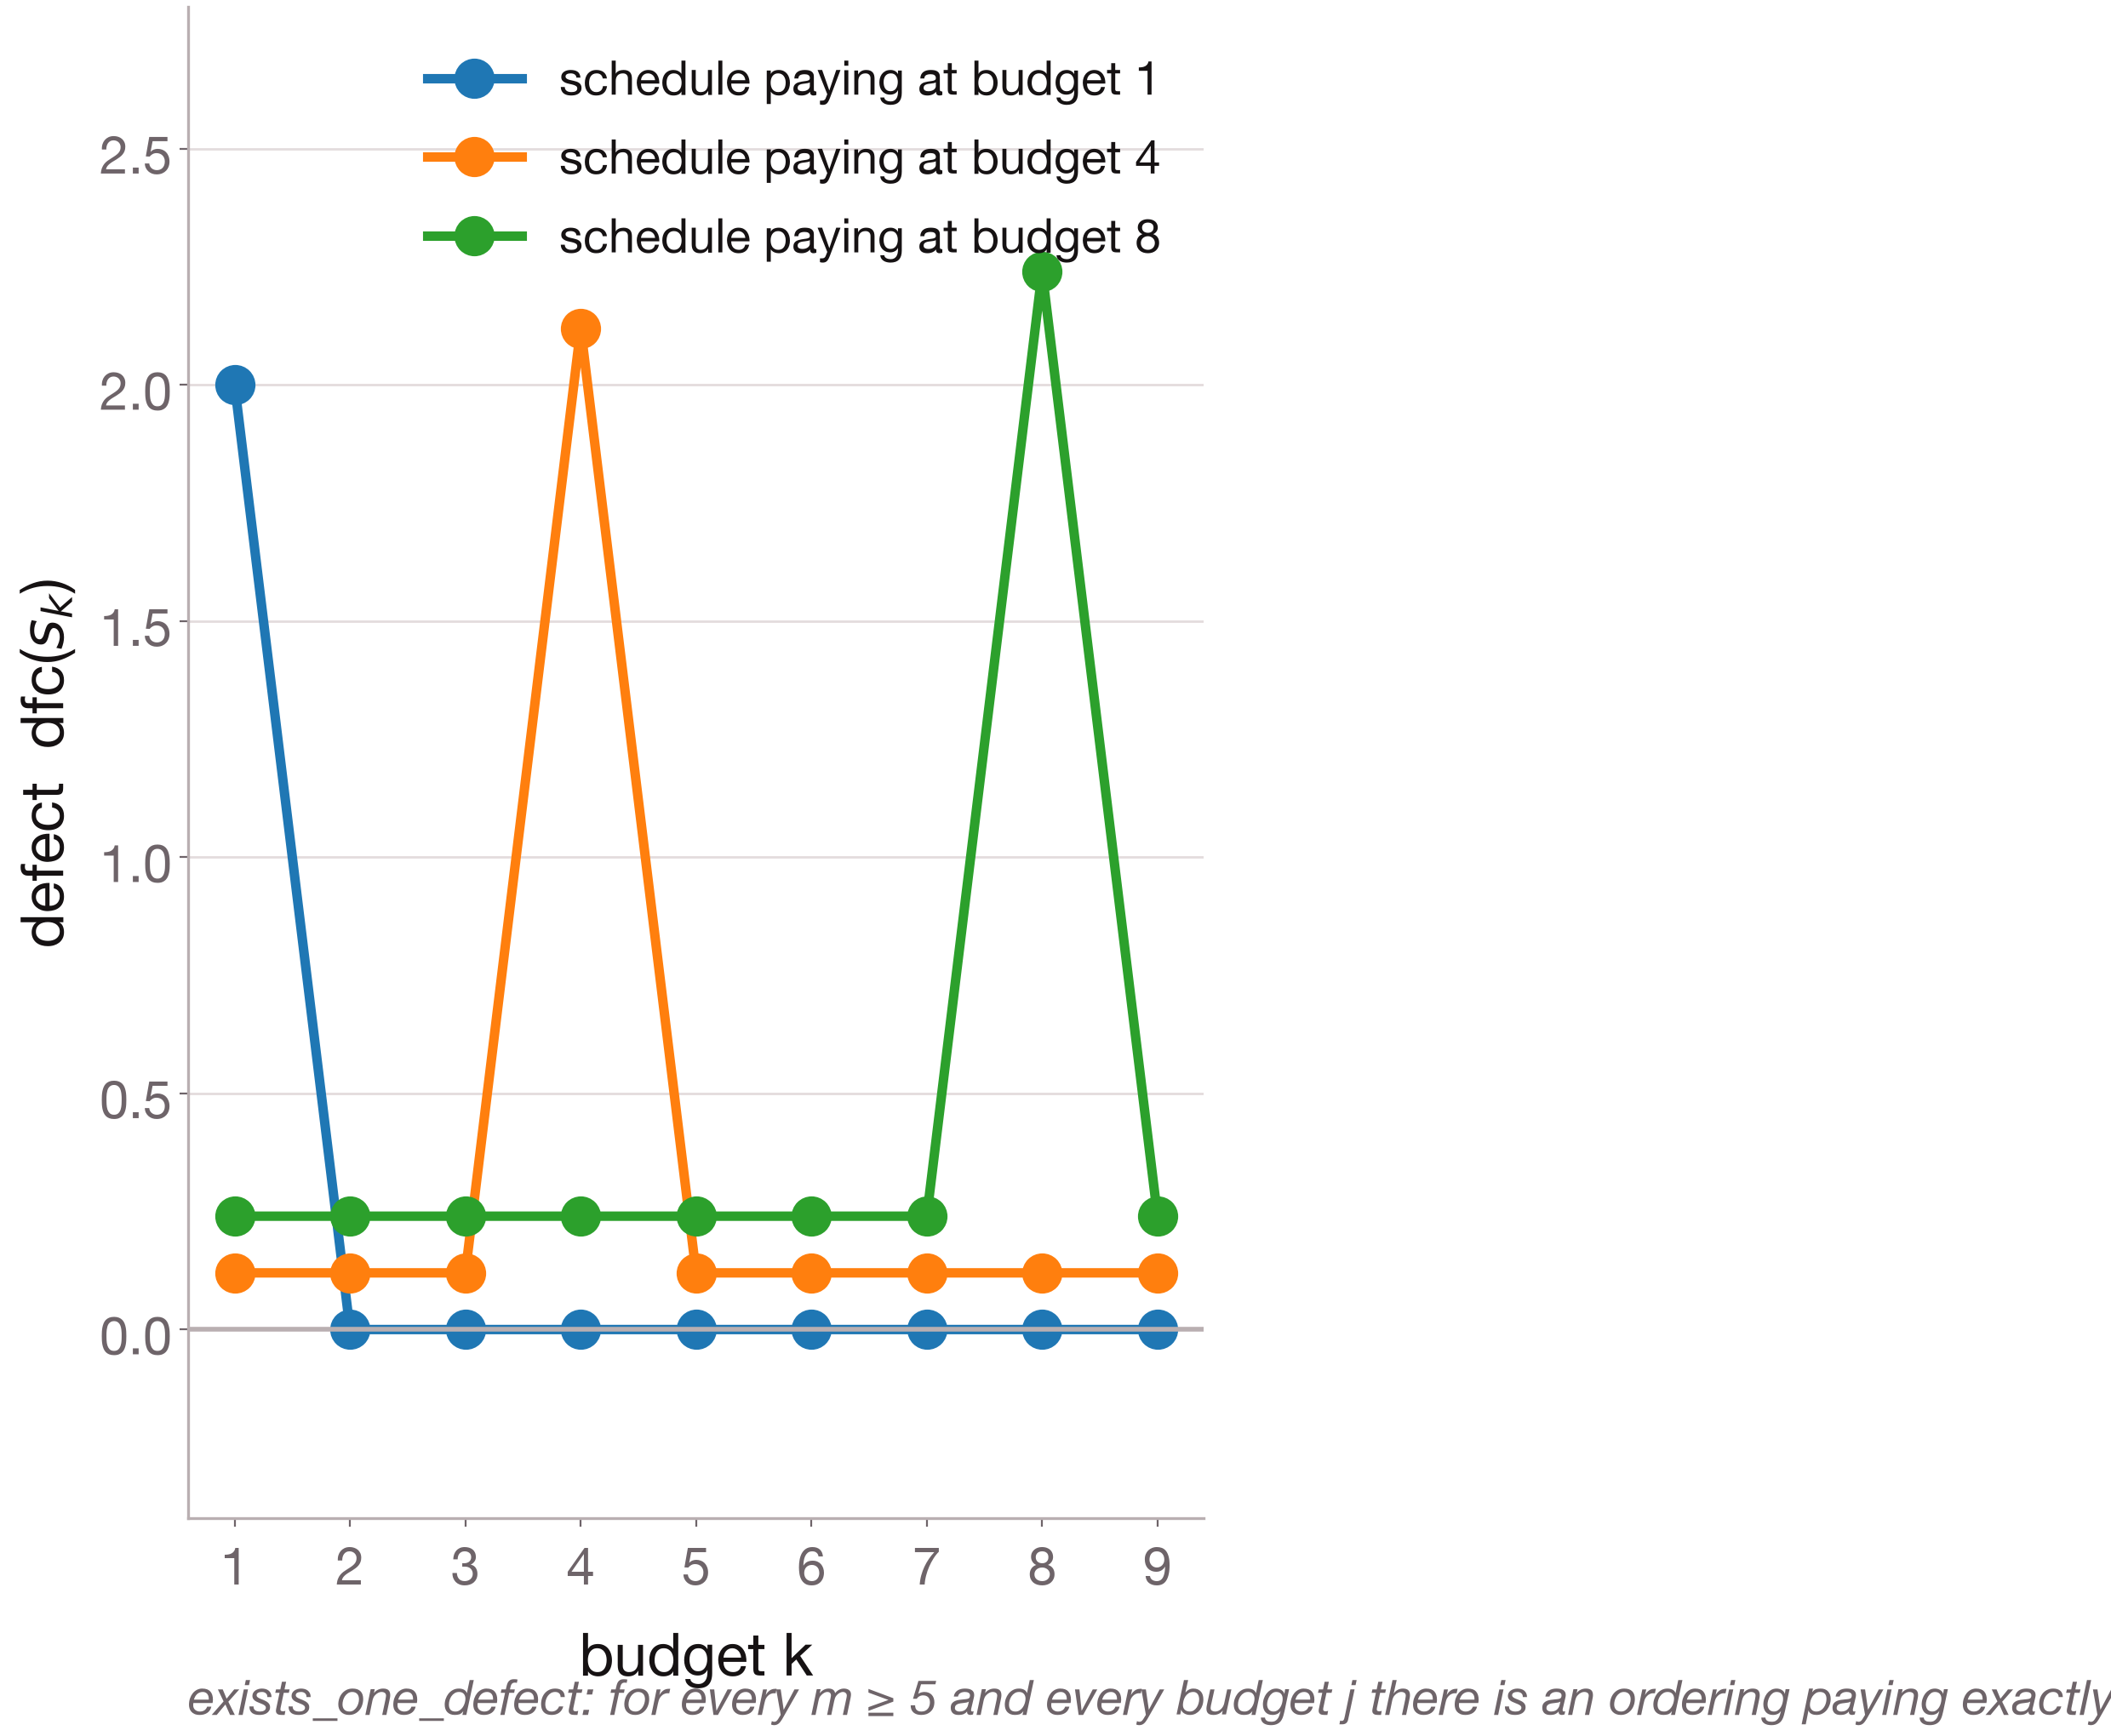
\includegraphics[width=\columnwidth]{struct_fig2_defect.png}
\caption{The one-defect construction of Theorem~\ref{thm:construction}. For every $m\ge5$ and
every budget $j$ there is an ordering paying exactly $2$, and paying it exactly at $j$.}
\label{fig:defect}
\end{figure}

\subsection{The Law}
\label{sec:law}

\begin{theorem}[Exact menu law]
\label{thm:law}
For every $m\ge5$,
\begin{equation}
V_{\mathrm{avg}}=\frac{2}{(m+4)(m-1)},\qquad
V_{\mathrm{path}}=\frac{2}{m+4},
\label{eq:law}
\end{equation}
and consequently
\begin{equation}
\frac{V_{\mathrm{path}}}{V_{\mathrm{avg}}}\;=\;m-1 .
\label{eq:ratio}
\end{equation}
\end{theorem}

\begin{proof}
By Theorem~\ref{thm:everyorderpays} the guaranteed payment is $c=2$, the normalisation in
\eqref{eq:regret} divides by $D=m+4$, and $|\mathrm{Bud}|=m-1$. Substituting into
\eqref{eq:bounds} gives the two values as lower bounds, and
Theorem~\ref{thm:attained}---whose witness exists by Theorem~\ref{thm:construction}---shows
both are achieved.
\end{proof}

\leanbox{\lean{ratio\_card\_concentrated\_on\_support} in
\lean{LeanStructuralFamilyLowerV1}}

\noindent\emph{Supporting results in \lean{LeanStructuralFamilyLowerV1}.}~The statements below supply the inequalities the step chains; produce the objects the step needs and supply the rewrites it performs, reproduced as the prover has them: Unicode maps to the corresponding \LaTeX{} symbol and identifiers are set upright, but no structure is rewritten and no hypothesis is dropped. A further $4$ audited declarations in this module are positivity checks and measurability side conditions, which carry no mathematical content of their own and are not displayed.

\noindent\textbf{S\,1}\quad\lean{avg\_lower}
{\footnotesize\[ \begin{aligned}[t]
&(\mathit{r} : \mathit{Ord} \to \mathit{Bud} \to \mathbb{R}\\
&\quad ),\; (\mathit{P} : \mathit{Ord} \to \mathbb{R} ),\; (\mathit{c} : \mathbb{R}\\
&\quad ),\; (\mathit{hr} : \forall \mathit{pi} \mathit{k}, 0 \leq \mathit{r} \mathit{pi}\\
&\quad \mathit{k}),\; (\mathit{hP} : \forall \mathit{pi}, 0 \leq \mathit{P}\\
&\quad \mathit{pi}),\; (\mathit{hsum} : \textstyle\sum \mathit{pi}, \mathit{P} \mathit{pi} =\\
&\quad 1),\; (\mathit{hcost} : \forall \mathit{pi}, \mathit{c} \leq \textstyle\sum \mathit{k}, \mathit{r} \mathit{pi}\\
&\quad \mathit{k})
\end{aligned} \]}
{\footnotesize\[ \begin{aligned}[t]
\vdash\;&\mathit{c} / (\mathit{Fintype}.\mathit{card} \mathit{Bud} : \mathbb{R}\\
&\quad ) \leq (\mathit{univ} : \mathit{Finset}\\
&\quad \mathit{Bud}).\mathit{sup'} \mathit{univ\_{}nonempty} (\mathbf{fun} \mathit{k} => \textstyle\sum \mathit{pi}, \mathit{P} \mathit{pi} * \mathit{r} \mathit{pi}\\
&\quad \mathit{k})
\end{aligned} \]}

\noindent\textbf{S\,2}\quad\lean{defects\_append}
{\footnotesize\[ \begin{aligned}[t]
&(\mathit{s} : \mathbb{Z} ),\; (\mathit{l₁} \mathit{l₂} : \mathit{List} \mathbb{Z}\\
&\quad )
\end{aligned} \]}
{\footnotesize\[ \begin{aligned}[t]
\vdash\;&\mathit{defects} \mathit{s} (\mathit{l₁} ++\\
&\quad \mathit{l₂}) = \mathit{defects} \mathit{s} \mathit{l₁}\\
&\quad ++ \mathit{defects} (\mathit{s} +\\
&\quad \mathit{l₁}.\mathit{sum}) \mathit{l₂}
\end{aligned} \]}

\noindent\textbf{S\,3}\quad\lean{dfc\_eq\_zero\_iff}
{\footnotesize\[ \begin{aligned}[t]
&(\mathit{s} : \mathbb{Z} )
\end{aligned} \]}
{\footnotesize\[ \begin{aligned}[t]
\vdash\;&\mathit{dfc} \mathit{s} = 0 \leftrightarrow |\mathit{s}|\\
&\quad \leq 1
\end{aligned} \]}

\noindent\textbf{S\,4}\quad\lean{dfc\_even}
{\footnotesize\[ \begin{aligned}[t]
&(\mathit{s} : \mathbb{Z} )
\end{aligned} \]}
{\footnotesize\[ \begin{aligned}[t]
\vdash\;&\mathit{dfc} \mathit{s} \% 2 = 0
\end{aligned} \]}

\noindent\textbf{S\,5}\quad\lean{no\_big\_step}
{\footnotesize\[ \begin{aligned}[t]
&(\mathit{s} : \mathbb{Z} ),\; (\mathit{l} : \mathit{List} \mathbb{Z}\\
&\quad ),\; (\mathit{hs} : |\mathit{s}| \leq 1),\; (\mathit{he} : |\mathit{s} + \mathit{l}.\mathit{sum}| \leq 1),\; (\mathit{h0} : \mathit{totalDefect} \mathit{s} \mathit{l} =\\
&\quad 0)
\end{aligned} \]}
{\footnotesize\[ \begin{aligned}[t]
\vdash\;&\forall \mathit{x} \in \mathit{l}, |\mathit{x}|\\
&\quad \leq 2
\end{aligned} \]}

\noindent\textbf{S\,6}\quad\lean{parity\_bridge}
{\footnotesize\[ \begin{aligned}[t]
&(\mathit{s} : \mathbb{Z} ),\; (\mathit{k} : \mathbb{N}\\
&\quad ),\; (\mathit{h} : \mathit{s} \% 2 = (\mathit{k} : \mathbb{Z} ) \%\\
&\quad 2)
\end{aligned} \]}
{\footnotesize\[ \begin{aligned}[t]
\vdash\;&\mathit{dfc} \mathit{s} = |\mathit{s}| - (\mathit{k} : \mathbb{Z}\\
&\quad ) \% 2
\end{aligned} \]}

\noindent\textbf{S\,7}\quad\lean{path\_lower}
{\footnotesize\[ \begin{aligned}[t]
&(\mathit{r} : \mathit{Ord} \to \mathit{Bud} \to \mathbb{R}\\
&\quad ),\; (\mathit{P} : \mathit{Ord} \to \mathbb{R} ),\; (\mathit{c} : \mathbb{R}\\
&\quad ),\; (\mathit{hP} : \forall \mathit{pi}, 0 \leq \mathit{P}\\
&\quad \mathit{pi}),\; (\mathit{hsum} : \textstyle\sum \mathit{pi}, \mathit{P} \mathit{pi} =\\
&\quad 1),\; (\mathit{hcost} : \forall \mathit{pi}, \exists \mathit{k}, \mathit{c} \leq \mathit{r} \mathit{pi}\\
&\quad \mathit{k})
\end{aligned} \]}
{\footnotesize\[ \begin{aligned}[t]
\vdash\;&\mathit{c} \leq \textstyle\sum \mathit{pi}, \mathit{P}\\
&\quad \mathit{pi} * ((\mathit{univ} : \mathit{Finset} \mathit{Bud}).\mathit{sup'} \mathit{univ\_{}nonempty} (\mathbf{fun} \mathit{k} => \mathit{r} \mathit{pi}\\
&\quad \mathit{k}))
\end{aligned} \]}

\noindent\textbf{S\,8}\quad\lean{ratio\_card\_concentrated\_on\_support}
{\footnotesize\[ \begin{aligned}[t]
&(\mathit{r} : \mathit{Ord} \to \mathit{Bud} \to \mathbb{R}\\
&\quad ),\; (\mathit{P} : \mathit{Ord} \to \mathbb{R} ),\; (\mathit{e} : \mathbb{R}\\
&\quad ),\; (\mathit{hP} : \forall \mathit{pi}, 0 \leq \mathit{P}\\
&\quad \mathit{pi}),\; (\mathit{hbal} : \forall \mathit{k}, (\textstyle\sum \mathit{pi}, \mathit{P} \mathit{pi} * \mathit{r} \mathit{pi} \mathit{k}) =\\
&\quad \mathit{e}),\; (\mathit{hconc} : \forall \mathit{pi}, \mathit{P} \mathit{pi} \neq 0 \to (\textstyle\sum \mathit{k}, \mathit{r} \mathit{pi} \mathit{k}) = (\mathit{univ} : \mathit{Finset} \mathit{Bud}).\mathit{sup'} \mathit{univ\_{}nonempty} (\mathbf{fun} \mathit{k} => \mathit{r} \mathit{pi}\\
&\quad \mathit{k}))
\end{aligned} \]}
{\footnotesize\[ \begin{aligned}[t]
\vdash\;&(\textstyle\sum \mathit{pi}, \mathit{P} \mathit{pi} * ((\mathit{univ} : \mathit{Finset} \mathit{Bud}).\mathit{sup'} \mathit{univ\_{}nonempty} (\mathbf{fun} \mathit{k} => \mathit{r} \mathit{pi}\\
&\quad \mathit{k}))) = (\mathit{Fintype}.\mathit{card} \mathit{Bud} : \mathbb{R}\\
&\quad ) * (\mathit{univ} : \mathit{Finset}\\
&\quad \mathit{Bud}).\mathit{sup'} \mathit{univ\_{}nonempty} (\mathbf{fun} \mathit{k} => \textstyle\sum \mathit{pi}, \mathit{P} \mathit{pi} * \mathit{r} \mathit{pi}\\
&\quad \mathit{k})
\end{aligned} \]}

\noindent\textbf{S\,9}\quad\lean{totalDefect\_even}
{\footnotesize\[ \begin{aligned}[t]
&(\mathit{s} : \mathbb{Z} ),\; (\mathit{l} : \mathit{List} \mathbb{Z}\\
&\quad )
\end{aligned} \]}
{\footnotesize\[ \begin{aligned}[t]
\vdash\;&\mathit{totalDefect} \mathit{s} \mathit{l} \% 2\\
&\quad = 0
\end{aligned} \]}

\noindent\textbf{S\,10}\quad\lean{two\_le\_dfc}
{\footnotesize\[ \begin{aligned}[t]
&(\mathit{s} : \mathbb{Z} ),\; (\mathit{h} : 2 \leq |\mathit{s}|)
\end{aligned} \]}
{\footnotesize\[ \begin{aligned}[t]
\vdash\;&2 \leq \mathit{dfc} \mathit{s}
\end{aligned} \]}

\noindent\textbf{S\,11}\quad\lean{two\_le\_totalDefect}
{\footnotesize\[ \begin{aligned}[t]
&(\mathit{s} : \mathbb{Z} ),\; (\mathit{l} : \mathit{List} \mathbb{Z}\\
&\quad ),\; (\mathit{hs} : |\mathit{s}| \leq 1),\; (\mathit{he} : |\mathit{s} + \mathit{l}.\mathit{sum}| \leq 1),\; (\mathit{h3} : \exists \mathit{x} \in \mathit{l}, 2 <\\
&\quad |\mathit{x}|)
\end{aligned} \]}
{\footnotesize\[ \begin{aligned}[t]
\vdash\;&2 \leq \mathit{totalDefect} \mathit{s} \mathit{l}
\end{aligned} \]}


The assembly carries two hypotheses, balance and concentration, which say that the
expectation of the maximum equals $|\mathrm{Bud}|$ times the maximum of the expectation. Both
are satisfied by the witness and are required only on the \emph{support} of the mixture; the
lower bounds still quantify over all permutations, so the law is not weakened by restricting
the witness.

\subsection{Does the Difficulty Survive Normalisation and Slack?}
\label{sec:tolerance}

Two objections meet any lower bound of this form. The first is that the instance might win by
inflating its coefficients, so the difficulty is an artefact of scale. The second is that
exact optimality is brittle, and that allowing a small regret $\varepsilon$ might collapse the
menu to one. Both are answered on an explicit scalar witness.

\begin{theorem}[Grid tolerance]
\label{thm:grid}
Let $\mathrm{cost}:2^{I}\to\mathbb{N}$ be integer-valued, let $\sigma>0$, and suppose
$\sigma\varepsilon<1$. If $S$ is $\varepsilon$-optimal at budget $k$ for
$T\mapsto\mathrm{cost}(T)/\sigma$, then $S$ is \emph{exactly} optimal at $k$.
\end{theorem}

\begin{proof}
$\varepsilon$-optimality gives $\mathrm{cost}(S)\le\mathrm{cost}(T)+\sigma\varepsilon
<\mathrm{cost}(T)+1$ for every competitor $T$. Both sides are integers, so
$\mathrm{cost}(S)\le\mathrm{cost}(T)$.
\end{proof}

\leanbox{\lean{epsilonOptimal\_on\_grid} in \lean{LeanStructuralIntegerToleranceV1}}

The content is that below one grid unit, slack buys nothing: an objective whose values live
on a lattice of spacing $1/\sigma$ has no $\varepsilon$-optimal set that is not optimal. This
is the mechanism by which an exact lower bound extends to a band of tolerances, and it is
stated for a general quantised objective because the extension is not specific to this
witness.

\begin{proposition}[Normalised form]
\label{prop:normform}
For the seven-relation scalar witness $F_{7}$, dividing the component functions by $57$ so
that $\sum_{j}\mathrm{osc}(f_{j})/2=1$ gives
\begin{equation}
\widetilde{L}(S)\;=\;\frac{\mathrm{selectedRadius}(F_{7},S)}{57}
\;=\;\frac{\bigl|\,\mathrm{complementAbs}_{7}(S)\,\bigr|}{114}.
\label{eq:normform}
\end{equation}
\end{proposition}

\leanbox{\lean{normalized\_formula} in \lean{LeanStructuralIntegerToleranceV1}}

The right-hand side is an integer divided by $114$, so the normalised objective is quantised
at $\sigma=114$ and Theorem~\ref{thm:grid} applies for every $\varepsilon<1/114$.

\begin{theorem}[Five rankings remain necessary on a band]
\label{thm:fiveband}
For every $\varepsilon$ with $0\le\varepsilon<\tfrac{1}{114}$,
\begin{equation}
\chi_{\varepsilon}\bigl(\widetilde{L}\bigr)\;\geq\;5 .
\label{eq:fiveband}
\end{equation}
\end{theorem}

\begin{proof}
Suppose four rankings cover every budget to within $\varepsilon$. By
Proposition~\ref{prop:normform} the objective is $\mathrm{complementAbs}_{7}/114$, so
Theorem~\ref{thm:grid} with $\sigma=114$ upgrades every $\varepsilon$-optimal prefix in the
menu to an exactly optimal one. The menu therefore covers every budget exactly with four
rankings, which the exact lower bound for this witness forbids.
\end{proof}

\leanbox{\lean{normalized\_chi\_at\_least\_five} in
\lean{LeanStructuralIntegerToleranceV1}}

\noindent\emph{Supporting results in \lean{LeanStructuralIntegerToleranceV1}.}~The statements below supply the inequalities the step chains and the rewrites it performs, reproduced as the prover has them: Unicode maps to the corresponding \LaTeX{} symbol and identifiers are set upright, but no structure is rewritten and no hypothesis is dropped. A further $0$ audited declarations in this module are positivity checks and measurability side conditions, which carry no mathematical content of their own and are not displayed.

\noindent\textbf{S\,23}\quad\lean{epsilonOptimal\_on\_grid}
{\footnotesize\[ \begin{aligned}[t]
&(\mathit{cost} : \mathit{Finset} \mathit{I} \to \mathbb{N}\\
&\quad ),\; (\mathit{scale} \mathit{eps} : \mathbb{R} ),\; (\mathit{hscale} : 0 <\\
&\quad \mathit{scale}),\; (\mathit{heps} : \mathit{scale} * \mathit{eps} <\\
&\quad 1),\; (\mathit{k} : \mathbb{N} ),\; (\mathit{S} : \mathit{Finset}\\
&\quad \mathit{I}),\; (\mathit{h} : \mathit{EpsilonOptimalAt} (\mathbf{fun} \mathit{T} => (\mathit{cost} \mathit{T}:\mathbb{R} )/\mathit{scale}) \mathit{eps} \mathit{k}\\
&\quad \mathit{S})
\end{aligned} \]}
{\footnotesize\[ \begin{aligned}[t]
\vdash\;&\mathit{EpsilonOptimalAt} (\mathbf{fun} \mathit{T} => (\mathit{cost} \mathit{T}:\mathbb{R}\\
&\quad )/\mathit{scale}) 0 \mathit{k} \mathit{S}
\end{aligned} \]}

\noindent\textbf{S\,24}\quad\lean{normalized\_chi\_at\_least\_five}
{\footnotesize\[ \begin{aligned}[t]
&(\mathit{eps} : \mathbb{R} ),\; (\mathit{heps} : \mathit{eps} <\\
&\quad 1/114)
\end{aligned} \]}
{\footnotesize\[ \begin{aligned}[t]
\vdash\;&\neg \mathit{PrefixCoverDimensionAtMost}\\
&\quad \mathit{normalizedScalarObjective} \mathit{eps} 4
\end{aligned} \]}

\noindent\textbf{S\,25}\quad\lean{normalized\_formula}
{\footnotesize\[ \begin{aligned}[t]
&(\mathit{S} : \mathit{Finset} (\mathit{Fin} 7))
\end{aligned} \]}
{\footnotesize\[ \begin{aligned}[t]
\vdash\;&\mathit{normalizedScalarObjective} \mathit{S}\\
&\quad = (\mathit{complementAbs7} \mathit{S}:\mathbb{R} )/114
\end{aligned} \]}


The normalisation objection is met outright, since \eqref{eq:normform} is stated after
dividing by the total radius. The slack objection is met on a band rather than on all
$\varepsilon$: five rankings are necessary up to $1/114$ and no further. The honest statement
is that exact-optimality difficulty is robust to a \emph{quantified} amount of slack,
computed from the objective's lattice rather than found by a sweep.

\subsection{The Constrained Problem}
\label{sec:marginal}

A natural objection is that the law might not survive a prescribed marginal---a requirement
that each item be retained with a given frequency. The object at issue is not a scalar per
budget but a trajectory.

\begin{definition}[Retained trajectory]
For a menu $\{\pi_{j}\}_{j\in J}$,
\begin{equation}
x^{*}_{i,k}\;=\;\frac{1}{|J|}\,
  \#\bigl\{\,j\;:\;i\in\mathrm{prefix}(\pi_{j},k)\,\bigr\}.
\label{eq:marginal}
\end{equation}
\end{definition}

The matrix form is used rather than a scalar summary because under signed cancellation two
menus can deliver the same expected value at every budget while retaining different items,
and \eqref{eq:regret} depends on the retained set through $|s_{k}|$, not on any scalar
summary of it. A constraint stated on a scalar therefore fails to constrain the object that
determines the objective.

\begin{theorem}[Column identity, for every menu]
\label{thm:colsum}
For every menu and every budget $k$, $\sum_{i}x^{*}_{i,k}=\min(k,n)$.
\end{theorem}

\begin{proof}
A length-$k$ prefix holds exactly $\min(k,n)$ items. Summing \eqref{eq:marginal} over items
and exchanging the two finite sums gives $\frac{1}{|J|}\sum_{j}\min(k,n)=\min(k,n)$.
\end{proof}

\leanbox{\lean{card\_prefixSet}, \lean{retained\_col\_sum} in
\lean{LeanStructuralRetainedMarginalV1}}

\begin{theorem}[The cyclic menu, in closed form]
\label{thm:cyclic}
On the cyclic menu, $x^{*}_{i,k}=\min(k,m)/m$ for every item $i$.
\end{theorem}

\leanbox{\lean{cyclic\_retained}, \lean{retained\_transfer} in
\lean{LeanStructuralRetainedMarginalV1}}

\noindent\emph{Supporting results in \lean{LeanStructuralRetainedMarginalV1}.}~The statements below supply the inequalities the step chains; produce the objects the step needs and supply the rewrites it performs, reproduced as the prover has them: Unicode maps to the corresponding \LaTeX{} symbol and identifiers are set upright, but no structure is rewritten and no hypothesis is dropped. A further $1$ audited declarations in this module are positivity checks and measurability side conditions, which carry no mathematical content of their own and are not displayed.

\noindent\textbf{S\,26}\quad\lean{card\_prefixSet}
{\footnotesize\[ \begin{aligned}[t]
&(\mathit{pos} : \alpha \to \mathbb{N} ),\; (\mathit{h} : \mathit{IsRanking}\\
&\quad \mathit{pos}),\; (\mathit{k} : \mathbb{N} )
\end{aligned} \]}
{\footnotesize\[ \begin{aligned}[t]
\vdash\;&(\mathit{prefixSet} \mathit{pos}\\
&\quad \mathit{k}).\mathit{card} = \mathit{min} \mathit{k} (\mathit{Fintype}.\mathit{card} \alpha )
\end{aligned} \]}

\noindent\textbf{S\,27}\quad\lean{cyclic\_retained}
{\footnotesize\[ \begin{aligned}[t]
&(\mathit{i} : \mathit{ZMod} \mathit{m}),\; (\mathit{k} : \mathbb{N}\\
&\quad )
\end{aligned} \]}
{\footnotesize\[ \begin{aligned}[t]
\vdash\;&\mathit{retained} (\alpha
\end{aligned} \]}

\noindent\textbf{S\,28}\quad\lean{retained\_col\_sum}
{\footnotesize\[ \begin{aligned}[t]
&[\mathit{Nonempty} \mathit{J}],\; (\mathit{pos} : \mathit{J} \to \alpha \to \mathbb{N}\\
&\quad ),\; (\mathit{hpos} : \forall \mathit{j}, \mathit{IsRanking} (\mathit{pos}\\
&\quad \mathit{j})),\; (\mathit{k} : \mathbb{N} )
\end{aligned} \]}
{\footnotesize\[ \begin{aligned}[t]
\vdash\;&\textstyle\sum \mathit{i} : \alpha , \mathit{retained}\\
&\quad \mathit{pos} \mathit{i} \mathit{k} = ((\mathit{min} \mathit{k} (\mathit{Fintype}.\mathit{card} \alpha ) : \mathbb{N} ) : \mathbb{R}\\
&\quad )
\end{aligned} \]}

\noindent\textbf{S\,29}\quad\lean{retained\_constrained\_eq\_free}
{\footnotesize\[ \begin{aligned}[t]
&(\mathit{val} : (\mathit{Ord} \to \mathbb{R} ) \to \mathbb{R}\\
&\quad ),\; (\mathit{Feasible} : (\mathit{Ord} \to \mathbb{R} ) \to \mathit{Prop}),\; (\mathit{traj} : (\mathit{Ord} \to \mathbb{R} ) \to \alpha \to \mathbb{N} \to \mathbb{R}\\
&\quad ),\; (\mathit{target} : \alpha \to \mathbb{N} \to \mathbb{R}\\
&\quad ),\; (\mathit{V} : \mathbb{R} ),\; (\mathit{P₀} : \mathit{Ord} \to \mathbb{R}\\
&\quad ),\; (\mathit{hfree} : \forall \mathit{P}, \mathit{Feasible} \mathit{P} \to \mathit{V} \leq \mathit{val}\\
&\quad \mathit{P}),\; (\mathit{hF₀} : \mathit{Feasible}\\
&\quad \mathit{P₀}),\; (\mathit{hT₀} : \forall \mathit{i} \mathit{k}, \mathit{traj} \mathit{P₀} \mathit{i} \mathit{k} = \mathit{target} \mathit{i}\\
&\quad \mathit{k}),\; (\mathit{hval} : \mathit{val} \mathit{P₀} =\\
&\quad \mathit{V})
\end{aligned} \]}
{\footnotesize\[ \begin{aligned}[t]
\vdash\;&\mathit{IsLeast} \{ \mathit{v} | \exists \mathit{P},\\
&\quad \mathit{Feasible} \mathit{P} \wedge (\forall \mathit{i} \mathit{k}, \mathit{traj} \mathit{P} \mathit{i} \mathit{k} = \mathit{target} \mathit{i}\\
&\quad \mathit{k}) \wedge \mathit{val} \mathit{P} =\\
&\quad \mathit{v}\} \mathit{V}
\end{aligned} \]}

\noindent\textbf{S\,30}\quad\lean{retained\_le\_one}
{\footnotesize\[ \begin{aligned}[t]
&[\mathit{Nonempty} \mathit{J}],\; (\mathit{pos} : \mathit{J} \to \alpha \to \mathbb{N}\\
&\quad ),\; (\mathit{i} : \alpha ),\; (\mathit{k} : \mathbb{N}\\
&\quad )
\end{aligned} \]}
{\footnotesize\[ \begin{aligned}[t]
\vdash\;&\mathit{retained} \mathit{pos} \mathit{i} \mathit{k}\\
&\quad \leq 1
\end{aligned} \]}

\noindent\textbf{S\,31}\quad\lean{retained\_mono}
{\footnotesize\[ \begin{aligned}[t]
&(\mathit{pos} : \mathit{J} \to \alpha \to \mathbb{N}\\
&\quad ),\; (\mathit{i} : \alpha ),\; \{ \mathit{k} \mathit{l}\\
&\quad : \mathbb{N} \},\; (\mathit{hkl} : \mathit{k} \leq \mathit{l})
\end{aligned} \]}
{\footnotesize\[ \begin{aligned}[t]
\vdash\;&\mathit{retained} \mathit{pos} \mathit{i} \mathit{k}\\
&\quad \leq \mathit{retained} \mathit{pos} \mathit{i}\\
&\quad \mathit{l}
\end{aligned} \]}

\noindent\textbf{S\,32}\quad\lean{retained\_transfer}
{\footnotesize\[ \begin{aligned}[t]
&(\mathit{val} : (\mathit{Ord} \to \mathbb{R} ) \to \mathbb{R}\\
&\quad ),\; (\mathit{Feasible} : (\mathit{Ord} \to \mathbb{R} ) \to \mathit{Prop}),\; (\mathit{traj} : (\mathit{Ord} \to \mathbb{R} ) \to \alpha \to \mathbb{N} \to \mathbb{R}\\
&\quad ),\; (\mathit{target} : \alpha \to \mathbb{N} \to \mathbb{R}\\
&\quad ),\; (\mathit{V} : \mathbb{R} ),\; (\mathit{hfree} : \forall \mathit{P}, \mathit{Feasible} \mathit{P} \to \mathit{V} \leq \mathit{val}\\
&\quad \mathit{P})
\end{aligned} \]}
{\footnotesize\[ \begin{aligned}[t]
\vdash\;&\forall \mathit{P}, \mathit{Feasible} \mathit{P}\\
&\quad \to (\forall \mathit{i} \mathit{k}, \mathit{traj} \mathit{P} \mathit{i} \mathit{k} = \mathit{target} \mathit{i}\\
&\quad \mathit{k}) \to \mathit{V} \leq \mathit{val} \mathit{P}
\end{aligned} \]}


Theorem~\ref{thm:colsum} cuts both ways. It confirms that the uniform trajectory is
realisable rather than merely feasible on paper. But because it holds for \emph{every} menu
it singles out none, so a prescribed column sum cannot by itself exclude the witness of
Theorem~\ref{thm:attained}. What remains open is a prescribed \emph{non-uniform} trajectory.

\section{Formal Verification}
\label{sec:verification}

\subsection{Acceptance Contract}

A module counts as accepted only when all six of the following hold: the compiler exits zero
with no errors; the source hash is unchanged \emph{across} the compile, so the file checked is
the file on disk; the compiled artifact is newer than its source; at least one
\texttt{\#print axioms} directive is present; the axiom set of every audited declaration lies
within $\{\textsf{propext},\textsf{Classical.choice},\textsf{Quot.sound}\}$; and no
\texttt{sorry} appears anywhere in the file.

The contract is stated in full because each clause excludes a specific way of appearing
verified without being so. The hash check across the compile excludes editing a file after
checking it; the artifact-newer check excludes a stale \texttt{.olean}; and the axiom audit is
a \emph{whitelist} rather than a blacklist, so an axiom introduced by a decision procedure
outside the kernel is rejected by name mismatch rather than needing to be anticipated.

\subsection{Evidence per Step}

\begin{table}[htbp]
\caption{Evidence per step. All cited declarations are axiom-audited.}
\label{tab:inventory}
\centering\footnotesize\setlength{\tabcolsep}{3pt}
\begin{tabular}{@{}llr@{}}
\toprule
Step & Module & Aud. \\
\midrule
Defect, Thm~\ref{thm:parity}            & \lean{LeanStructuralFamilyLowerV1}      & 15 \\
Mechanism, Thm~\ref{thm:everyorderpays} & \lean{LeanStructuralFamilyLowerV1}      & 15 \\
Bounds, Thm~\ref{thm:bounds}            & \lean{LeanStructuralFamilyLowerV1}      & 15 \\
Attainment, Thm~\ref{thm:attained}      & \lean{LeanStructuralFamilyLowerV1}      & 15 \\
Construction, Thm~\ref{thm:construction}& \lean{LeanStructuralFamilyUpperV1}      & 11 \\
Tolerance, Thms~\ref{thm:grid}--\ref{thm:fiveband} & \lean{LeanStructuralIntegerToleranceV1} & 3 \\
Marginal, Thms~\ref{thm:colsum}--\ref{thm:cyclic} & \lean{LeanStructuralRetainedMarginalV1} & 8 \\
\bottomrule
\end{tabular}
\end{table}

\subsection{Scope of the Formalisation}

The Structural strand contains $77$ Lean source files with $959$ theorem and lemma
statements, of which $13$ modules carry an acceptance receipt covering $171$ audited
declarations. Across the programme: $762$ files, $7{,}199$ statements, $111$ accepted modules,
$875$ audited declarations.

One join is supplied by the paper rather than by a Lean name, and it is flagged here.
\lean{no\_big\_step} and \lean{two\_le\_totalDefect} are stated for an arbitrary
\lean{List $\mathbb{Z}$}, with ``some element exceeds $2$'' as a hypothesis. That every
ordering of $g_{m}$ is such a list---that permuting a multiset does not remove the element
$3$---is immediate and is carried out in the proof of Theorem~\ref{thm:everyorderpays}.
Quoting \lean{two\_le\_totalDefect} as though its conclusion were already about the family
would misdescribe what the prover checked. Every audited statement of every module this paper cites is displayed in Section~
ef{sec:setting}, attached to the step that uses it; only positivity checks and measurability side conditions are omitted, and their count is given at each block. The strand contains a further $9$ accepted modules carrying $118$ audited declarations that no step of this paper uses; they belong to other results of the programme. Appendix~\ref{app:inventory} reproduces the complete chain: all $155$ audited statements of the strand across its $13$ accepted modules, grouped by module.

\section{Experiments}

\subsection{Experimental Objectives}

Theorems~\ref{thm:everyorderpays} and \ref{thm:construction} quantify over all $m\ge5$, so no
enumeration can strengthen them. The enumeration has one objective: to confirm that the
defect definition used in the code and the one used in the proofs agree, which is the failure
mode a proved theorem does not protect against.

\subsection{Setup}

Every distinct ordering of $g_{m}$ was enumerated for $5\le m\le12$---$57{,}724$ orderings in
total---and each ordering's defect vector computed from \eqref{eq:dfcbridge} in exact integer
arithmetic. Orderings are enumerated up to multiset repetition; there is no sampling and no
floating point.

\subsection{Metrics}

Three aggregates are recorded per $m$: the minimum total defect over all orderings; the
minimum \emph{path} defect, that is, the minimum over orderings of the maximum per-budget
defect; and the set of budgets at which some ordering achieves a defect vector with a single
non-zero entry equal to $2$.

\subsection{Statistical Reporting}

Every quantity is deterministic and exact. The tabulated law values are exact rationals
evaluated in floating point for display only.

\section{Results}
\label{sec:results}

\subsection{Reporting Protocol}

All $m$ in range are reported with no exclusions, and the law is tabulated for $m=5$ to $20$
alongside.

\subsection{Every Ordering Pays, Checked Exhaustively}

The minimum total defect is $2$ at every $m$, so no ordering is free. The minimum path defect
is also $2$, so no ordering escapes by spreading a total of $2$ across several budgets at
lower cost each---which Corollary~\ref{cor:nocheap} already forbids and which the enumeration
confirms the implementation respects. One-defect schedules exist at every budget for every
$m$ in range, so the menu of Theorem~\ref{thm:attained} is realisable throughout.

\begin{table}[htbp]
\caption{Exhaustive enumeration of \emph{every} distinct ordering of $g_{m}$ for
$5\le m\le12$---57,724 orderings in total. The minimum total defect is $2$ at every $m$,
confirming Theorem~\ref{thm:everyorderpays}; the minimum path defect is also $2$, so no
ordering escapes by spreading its payment; and one-defect schedules exist at every budget,
confirming Theorem~\ref{thm:construction}. The Lean statements quantify over all $m\ge5$,
so this table checks the implementation rather than extending the theorems.}
\label{tab:enum}
\centering
\footnotesize
\setlength{\tabcolsep}{3pt}
\begin{tabular}{@{}rrrrrrcc@{}}
\toprule
$m$ & orderings & bud. & min tot. & min path & covered & pays & covers \\
\midrule
5 & 60 & 4 & 2 & 2 & 4 & yes & yes \\
6 & 180 & 5 & 2 & 2 & 5 & yes & yes \\
7 & 420 & 6 & 2 & 2 & 6 & yes & yes \\
8 & 1,120 & 7 & 2 & 2 & 7 & yes & yes \\
9 & 2,520 & 8 & 2 & 2 & 8 & yes & yes \\
10 & 6,300 & 9 & 2 & 2 & 9 & yes & yes \\
11 & 13,860 & 10 & 2 & 2 & 10 & yes & yes \\
12 & 33,264 & 11 & 2 & 2 & 11 & yes & yes \\
\bottomrule
\end{tabular}
\end{table}


\subsection{The Ratio Is Exactly $m-1$, and Both Levels Fall}

Table~\ref{tab:law} tabulates \eqref{eq:law} over $m=5$ to $20$. $V_{\mathrm{avg}}$ falls
from $1/18$ to $1/216$ and $V_{\mathrm{path}}$ from $2/9$ to $1/12$, while the ratio climbs
from $4$ to $19$. Both columns are exact rationals and the ratio column is
\eqref{eq:ratio} evaluated, not fitted.

\begin{figure}[htbp]
\centering
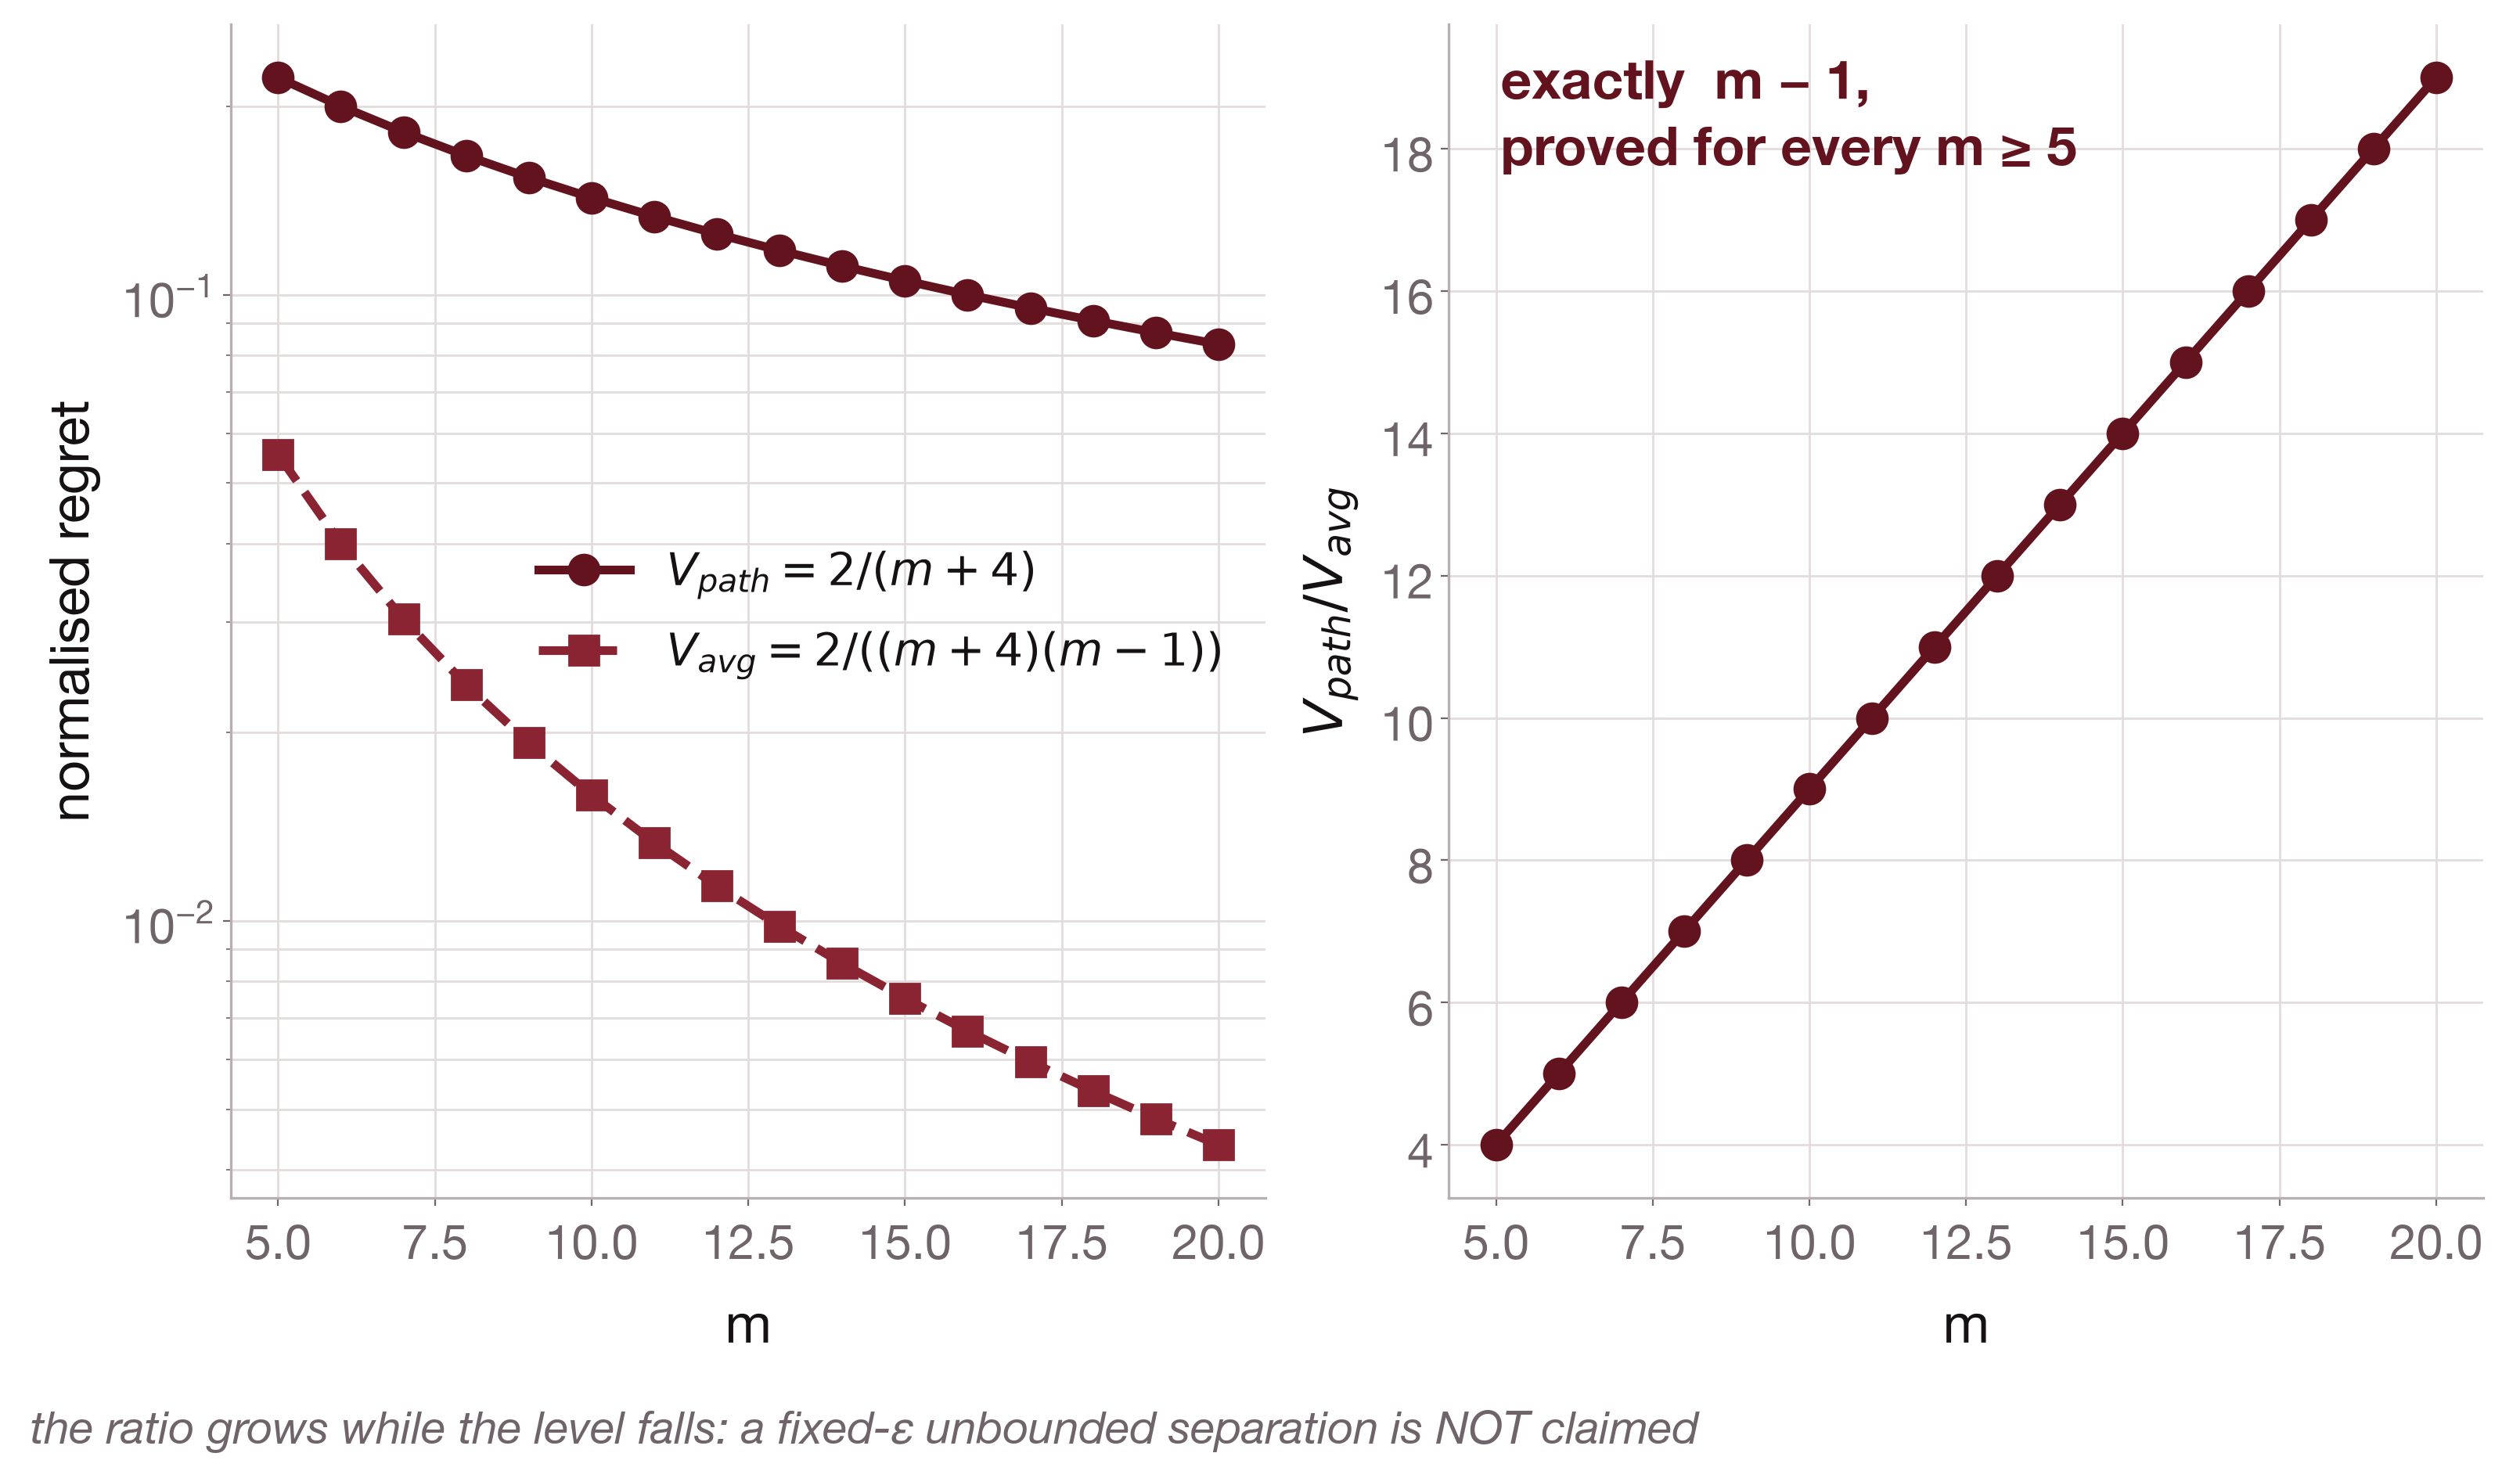
\includegraphics[width=\columnwidth]{struct_fig1_law.png}
\caption{The exact law of Theorem~\ref{thm:law}. Left: both values fall like $1/m$. Right:
their ratio is exactly $m-1$, proved for every $m\ge5$ rather than fitted.}
\label{fig:law}
\end{figure}

\begin{table*}[t]
\caption{The exact law \eqref{eq:law} tabulated for $m=5$ to $20$. Both value columns are
exact rationals evaluated in floating point, and the ratio column is $m-1$ at every row---
not fitted, but the identity \eqref{eq:ratio} evaluated. Both levels fall like $1/m$ while
the ratio grows linearly; Section~\ref{sec:results} is explicit that these two facts are
simultaneous, so no unbounded fixed-$\varepsilon$ separation is claimed.}
\label{tab:law}
\centering
\footnotesize
\setlength{\tabcolsep}{5pt}
\begin{tabular}{@{}rllllr@{\hspace{10pt}}|@{\hspace{10pt}}rllllr@{}}
\toprule
$m$ & $V_{\mathrm{avg}}$ & value & $V_{\mathrm{path}}$ & value & ratio & $m$ & $V_{\mathrm{avg}}$ & value & $V_{\mathrm{path}}$ & value & ratio \\
\midrule
5 & $\frac{2}{36}$ & 0.055556 & $\frac{2}{9}$ & 0.222222 & 4 & 13 & $\frac{2}{204}$ & 0.009804 & $\frac{2}{17}$ & 0.117647 & 12 \\
6 & $\frac{2}{50}$ & 0.040000 & $\frac{2}{10}$ & 0.200000 & 5 & 14 & $\frac{2}{234}$ & 0.008547 & $\frac{2}{18}$ & 0.111111 & 13 \\
7 & $\frac{2}{66}$ & 0.030303 & $\frac{2}{11}$ & 0.181818 & 6 & 15 & $\frac{2}{266}$ & 0.007519 & $\frac{2}{19}$ & 0.105263 & 14 \\
8 & $\frac{2}{84}$ & 0.023810 & $\frac{2}{12}$ & 0.166667 & 7 & 16 & $\frac{2}{300}$ & 0.006667 & $\frac{2}{20}$ & 0.100000 & 15 \\
9 & $\frac{2}{104}$ & 0.019231 & $\frac{2}{13}$ & 0.153846 & 8 & 17 & $\frac{2}{336}$ & 0.005952 & $\frac{2}{21}$ & 0.095238 & 16 \\
10 & $\frac{2}{126}$ & 0.015873 & $\frac{2}{14}$ & 0.142857 & 9 & 18 & $\frac{2}{374}$ & 0.005348 & $\frac{2}{22}$ & 0.090909 & 17 \\
11 & $\frac{2}{150}$ & 0.013333 & $\frac{2}{15}$ & 0.133333 & 10 & 19 & $\frac{2}{414}$ & 0.004831 & $\frac{2}{23}$ & 0.086957 & 18 \\
12 & $\frac{2}{176}$ & 0.011364 & $\frac{2}{16}$ & 0.125000 & 11 & 20 & $\frac{2}{456}$ & 0.004386 & $\frac{2}{24}$ & 0.083333 & 19 \\
\bottomrule
\end{tabular}
\end{table*}


\subsection{Reading the Two Trends Together}

Read carelessly, the ratio column alone suggests an unbounded separation. It is not one in
the sense that matters to a client, and the reason is that both quantities are normalised by
$D=m+4$: as the population grows, a single defect of $2$ becomes a smaller fraction of the
total weight, so the absolute regret under either objective shrinks. The ratio grows because
$V_{\mathrm{avg}}$ additionally divides by the number of budgets. A client with a fixed
absolute tolerance therefore finds both regimes acceptable once $m$ is large enough.

What does translate is the menu size. At every $m\ge5$, achieving $V_{\mathrm{avg}}$ rather
than $V_{\mathrm{path}}$ requires $m-1$ schedules rather than one, and that cost is paid in
full whatever the tolerance. The correct summary is not ``the gap grows'' but ``the gap is
exactly the menu size, at every population size''.

\section{Discussion}
\label{sec:discussion}

\subsection{What the Results Establish}

The gap between one schedule and a menu is not a constant factor but an exact function of the
population size. That is sharper than a competitive ratio, and it is available precisely
because both sides are attained, so no slack hides in either bound. The practical reading is
that under signed cancellation the right design object is the \emph{menu} and its
cardinality, not a single ordering. A designer who must publish one ordering is not choosing
a slightly worse one; by Theorem~\ref{thm:everyorderpays} they are choosing one that fails at
some budget, and the only question is which.

\subsection{Shortcomings and Limitations}

\emph{The law is for one family.} Assumption 2 generalises---the lower side holds for any odd
family containing an element above the band---but assumption 3 does not, since
Theorem~\ref{thm:construction} uses the specific counts \eqref{eq:familyparams}. A setting
satisfying the mechanism's hypotheses inherits the impossibility and not the identity.

\emph{The column identity singles out no menu.} Theorem~\ref{thm:colsum} holds for every
menu, so a prescribed uniform marginal excludes nothing. A prescribed non-uniform trajectory
may exclude the witness and change the value, and that case is open.

\emph{The cyclic menu is not shown optimal.} It is chosen for computability.

\emph{The assembly carries two hypotheses.} Theorem~\ref{thm:law} needs balance and
concentration on the support of the mixture. Both hold for the witness, but the law as stated
is not hypothesis-free.

\emph{No algorithm and no competitive ratio.} Nothing here is an online algorithm, and for
the reason given in the Background the usual competitive currency is unavailable.

\emph{The tolerance band is narrow.} Theorem~\ref{thm:fiveband} covers
$\varepsilon<1/114$ and says nothing above it; the difficulty does collapse for larger
slack.

\subsection{Open Problems}

Which families admit an exact law of this kind is the first question. The mechanism uses only
that some element exceeds $2$ while the rest are units, which suggests a class rather than an
instance; whether the \emph{attainment} side generalises is less clear.

The non-uniform prescribed trajectory is the second, and the one a referee is most likely to
press: the column identity settles the uniform case and nothing beyond it.

Third, the menu cardinality $m-1$ equals $|\mathrm{Bud}|$ here. Whether that coincidence is
structural or an artefact of this family is open, and the K-adaptability comparison of
Section~II suggests the answer depends on how badly concavity fails rather than on the family
alone.

\section{Conclusion}

Under signed cancellation, one schedule cannot serve every budget, and the exact price of
serving them all is a menu of $m-1$ schedules. Both values in the law are attained, so
$V_{\mathrm{path}}/V_{\mathrm{avg}}=m-1$ is an identity; the mechanism behind it needs no
side hypotheses and holds for every $m\ge5$; the one-defect schedules that realise it are
constructed rather than shown to exist; and the difficulty survives normalisation and a
quantified band of slack. The question a designer can ask before doing any work is whether
the item weights cancel. If they do not, one ordering suffices and the classical theory
applies. If they do, one ordering provably does not suffice, the deficit is bounded below by
a constant rather than made small by care, and the right response is to publish a menu whose
size is the number of budgets to be served.

\section*{Acknowledgment}

The formal development uses the Lean~4 theorem prover and the mathlib library.

\begin{thebibliography}{00}

\bibitem{bernstein2017} A. Bernstein, Y. Disser, M. Gro\ss{}, and S. Himburg, ``General
bounds for incremental maximization,'' in \emph{Proc. 44th Int. Colloq. Automata, Languages,
and Programming (ICALP)}, 2017.

\bibitem{disser2023} Y. Disser, M. Klimm, K. Schewior, and D. Weckbecker, ``Incremental
maximization,'' arXiv:2305.01310, 2023.

\bibitem{kurtz2026} J. Kurtz, ``Bounding the optimal number of policies for robust
K-adaptability,'' \emph{Math. Program.}, 2026.

\bibitem{borodin1998} A. Borodin and R. El-Yaniv, \emph{Online Computation and Competitive
Analysis}. Cambridge, U.K.: Cambridge Univ. Press, 1998.

\bibitem{nemhauser1978} G. L. Nemhauser, L. A. Wolsey, and M. L. Fisher, ``An analysis of
approximations for maximizing submodular set functions---I,'' \emph{Math. Program.},
vol.~14, pp.~265--294, 1978.

\bibitem{mathlib2020} The mathlib Community, ``The Lean mathematical library,'' in
\emph{Proc. 9th ACM SIGPLAN Int. Conf. Certified Programs and Proofs (CPP)}, 2020,
pp.~367--381.

\bibitem{demoura2021} L. de Moura and S. Ullrich, ``The Lean 4 theorem prover and
programming language,'' in \emph{Proc. 28th Int. Conf. Automated Deduction (CADE)}, 2021,
pp.~625--635.

\end{thebibliography}

\appendices
\section{Complete statement inventory}
\label{app:inventory}

The Structural strand contributes $155$ axiom-audited theorems and lemmas across its accepted modules. Those that any step of this paper uses are displayed in Section~\ref{sec:setting}, beside the step that consumes them. This appendix reproduces the \emph{complete} chain---every audited statement of the strand, grouped by module, including the ones already shown---so that the development can be read end to end without reassembling it from the body.

Each entry is a symbol-level transliteration of the Lean statement: Unicode maps to the corresponding \LaTeX{} symbol and identifiers are set upright, but no structure is rewritten and no hypothesis is dropped. Binders are listed as the prover has them and the turnstile $\vdash$ separates them from the conclusion. Every entry carries an acceptance receipt and an axiom audit confining it to $\{\textsf{propext},\textsf{Classical.choice},\textsf{Quot.sound}\}$; none contains \texttt{sorry}.

\vspace{4pt}\noindent\rule{\columnwidth}{0.4pt}\par\vspace{2pt}
\noindent\textbf{Module \lean{LeanStructuralAvgPathGapV1}}\par\vspace{3pt}

\noindent\textbf{A\,1}\quad\lean{avg\_le\_path}
{\footnotesize\[ \begin{aligned}[t]
&(\mathit{r} : \mathit{Ord} \to \mathit{Bud} \to \mathbb{R}\\
&\quad ),\; (\mathit{P} : \mathit{Ord} \to \mathbb{R}\\
&\quad ),\; (\mathit{hP} : \forall \mathit{pi}, 0 \leq \mathit{P}\\
&\quad \mathit{pi})
\end{aligned} \]}
{\footnotesize\[ \begin{aligned}[t]
\vdash\;&\mathit{avgVal} \mathit{r} \mathit{P}\\
&\quad \leq \mathit{pathVal} \mathit{r}\\
&\quad \mathit{P}
\end{aligned} \]}

\noindent\textbf{A\,2}\quad\lean{eps\_le\_card\_avg}
{\footnotesize\[ \begin{aligned}[t]
&(\mathit{r} : \mathit{Ord} \to \mathit{Bud} \to \mathbb{R}\\
&\quad ),\; (\mathit{P} : \mathit{Ord} \to \mathbb{R}\\
&\quad ),\; (\mathit{hr} : \forall \mathit{pi} \mathit{k}, 0\\
&\quad \leq \mathit{r} \mathit{pi}\\
&\quad \mathit{k}),\; (\mathit{hP} : \forall \mathit{pi}, 0\\
&\quad \leq \mathit{P} \mathit{pi}),\; (\mathit{hP1} :\\
&\quad \textstyle\sum \mathit{pi}, \mathit{P} \mathit{pi} =\\
&\quad 1)
\end{aligned} \]}
{\footnotesize\[ \begin{aligned}[t]
\vdash\;&\mathit{epsNest} \mathit{r} \leq (\mathit{Fintype}.\mathit{card}\\
&\quad \mathit{Bud} : \mathbb{R} ) *\\
&\quad \mathit{avgVal} \mathit{r} \mathit{P}
\end{aligned} \]}

\noindent\textbf{A\,3}\quad\lean{eps\_le\_path}
{\footnotesize\[ \begin{aligned}[t]
&(\mathit{r} : \mathit{Ord} \to \mathit{Bud} \to \mathbb{R}\\
&\quad ),\; (\mathit{P} : \mathit{Ord} \to \mathbb{R}\\
&\quad ),\; (\mathit{hP} : \forall \mathit{pi}, 0 \leq \mathit{P}\\
&\quad \mathit{pi}),\; (\mathit{hP1} : \textstyle\sum \mathit{pi},\\
&\quad \mathit{P} \mathit{pi} = 1)
\end{aligned} \]}
{\footnotesize\[ \begin{aligned}[t]
\vdash\;&\mathit{epsNest} \mathit{r} \leq \mathit{pathVal}\\
&\quad \mathit{r} \mathit{P}
\end{aligned} \]}

\noindent\textbf{A\,4}\quad\lean{gap\_exactly\_card}
{\footnotesize\[ \begin{aligned}[t]
&(\mathit{r} : \mathit{Ord} \to \mathit{Bud} \to \mathbb{R}\\
&\quad ),\; (\mathit{P} : \mathit{Ord} \to \mathbb{R}\\
&\quad ),\; (\mathit{hr} : \forall \mathit{pi} \mathit{k}, 0\\
&\quad \leq \mathit{r} \mathit{pi}\\
&\quad \mathit{k}),\; (\mathit{hP} : \forall \mathit{pi}, 0\\
&\quad \leq \mathit{P} \mathit{pi}),\; (\mathit{hP1} :\\
&\quad \textstyle\sum \mathit{pi}, \mathit{P} \mathit{pi} =\\
&\quad 1),\; (\mathit{hsat} : (\mathit{Fintype}.\mathit{card}\\
&\quad \mathit{Bud} : \mathbb{R} ) * \mathit{avgVal}\\
&\quad \mathit{r} \mathit{P} = \mathit{epsNest}\\
&\quad \mathit{r})
\end{aligned} \]}
{\footnotesize\[ \begin{aligned}[t]
\vdash\;&\mathit{pathVal} \mathit{r} \mathit{P}\\
&\quad = (\mathit{Fintype}.\mathit{card} \mathit{Bud} :\\
&\quad \mathbb{R} ) * \mathit{avgVal}\\
&\quad \mathit{r} \mathit{P}
\end{aligned} \]}

\noindent\textbf{A\,5}\quad\lean{path\_le\_card\_avg}
{\footnotesize\[ \begin{aligned}[t]
&(\mathit{r} : \mathit{Ord} \to \mathit{Bud} \to \mathbb{R}\\
&\quad ),\; (\mathit{P} : \mathit{Ord} \to \mathbb{R}\\
&\quad ),\; (\mathit{hr} : \forall \mathit{pi} \mathit{k}, 0\\
&\quad \leq \mathit{r} \mathit{pi}\\
&\quad \mathit{k}),\; (\mathit{hP} : \forall \mathit{pi}, 0\\
&\quad \leq \mathit{P} \mathit{pi})
\end{aligned} \]}
{\footnotesize\[ \begin{aligned}[t]
\vdash\;&\mathit{pathVal} \mathit{r} \mathit{P}\\
&\quad \leq (\mathit{Fintype}.\mathit{card} \mathit{Bud} :\\
&\quad \mathbb{R} ) * \mathit{avgVal}\\
&\quad \mathit{r} \mathit{P}
\end{aligned} \]}

\vspace{4pt}\noindent\rule{\columnwidth}{0.4pt}\par\vspace{2pt}
\noindent\textbf{Module \lean{LeanStructuralBudgetRecourseV1}}\par\vspace{3pt}

\noindent\textbf{A\,6}\quad\lean{deletion\_card}
{\footnotesize\[ \begin{aligned}[t]
&(\mathit{t} \mathit{u} : \mathit{Fin}\\
&\quad \mathit{r}),\; (\mathit{hne} : \mathit{t} \neq \mathit{u})
\end{aligned} \]}
{\footnotesize\[ \begin{aligned}[t]
\vdash\;&(\mathit{staircaseSelected} \mathit{t} \\\
&\quad \mathit{staircaseSelected}\\
&\quad \mathit{u}).\mathit{card} =\\
&\quad \mathit{u}.\mathit{val}-\mathit{t}.\mathit{val}+1
\end{aligned} \]}

\noindent\textbf{A\,7}\quad\lean{good\_decision\_forced}
{\footnotesize\[ \begin{aligned}[t]
&(\mathit{hr} : 0 < \mathit{r}),\; (\mathit{eps} :\\
&\quad \mathbb{R} ),\; (\mathit{heps} :\\
&\quad 2*(\mathit{r}:\mathbb{R} )*\mathit{eps} <\\
&\quad 1),\; (\mathit{t} : \mathit{Fin}\\
&\quad \mathit{r}),\; (\mathit{S} : \mathit{Finset}\\
&\quad (\mathit{StairRel} \mathit{r})),\; (\mathit{hS} :\\
&\quad \mathit{EpsilonOptimalAt} (\mathbf{fun} \mathit{T} =>\\
&\quad \mathit{selectedRadius} \mathit{staircaseF}\\
&\quad \mathit{T}/(\mathit{r}:\mathbb{R} )) \mathit{eps}\\
&\quad (\mathit{staircaseSelected} \mathit{t}).\mathit{card}\\
&\quad \mathit{S})
\end{aligned} \]}
{\footnotesize\[ \begin{aligned}[t]
\vdash\;&\mathit{S}=\mathit{staircaseSelected}\\
&\quad \mathit{t}
\end{aligned} \]}

\noindent\textbf{A\,8}\quad\lean{policy\_total}
{\footnotesize\[ \begin{aligned}[t]
&(\mathit{hr} : 0 < \mathit{r}),\; (\mathit{eps} :\\
&\quad \mathbb{R} ),\; (\mathit{heps} :\\
&\quad 2*(\mathit{r}:\mathbb{R} )*\mathit{eps} <\\
&\quad 1),\; (\mathit{n} : \mathbb{N} ),\; (\mathit{t} :\\
&\quad \mathbb{N} \to \mathit{Fin}\\
&\quad \mathit{r}),\; (\mathit{S} : \mathbb{N} \to \mathit{Finset}\\
&\quad (\mathit{StairRel} \mathit{r})),\; (\mathit{hS} :\\
&\quad \forall \mathit{i} \leq \mathit{n},\mathit{EpsilonOptimalAt}\\
&\quad (\mathbf{fun} \mathit{T} => \mathit{selectedRadius}\\
&\quad \mathit{staircaseF} \mathit{T}/(\mathit{r}:\mathbb{R}\\
&\quad )) \mathit{eps} (\mathit{staircaseSelected}\\
&\quad (\mathit{t} \mathit{i})).\mathit{card} (\mathit{S}\\
&\quad \mathit{i}))
\end{aligned} \]}
{\footnotesize\[ \begin{aligned}[t]
\vdash\;&(\textstyle\sum \mathit{i} \in \mathit{range}\\
&\quad \mathit{n},\mathit{recourse} (\mathit{S} \mathit{i})\\
&\quad (\mathit{S} (\mathit{i}+1))) =\\
&\quad \textstyle\sum \mathit{i} \in \mathit{range}\\
&\quad \mathit{n},\mathbf{if} \mathit{t}\\
&\quad \mathit{i}=\mathit{t} (\mathit{i}+1)\\
&\quad \mathbf{then} 0 \mathbf{else} 1
\end{aligned} \]}

\noindent\textbf{A\,9}\quad\lean{selected\_difference}
{\footnotesize\[ \begin{aligned}[t]
&(\mathit{t} \mathit{u} : \mathit{Fin}\\
&\quad \mathit{r}),\; (\mathit{hne} : \mathit{t} \neq \mathit{u})
\end{aligned} \]}
{\footnotesize\[ \begin{aligned}[t]
\vdash\;&\mathit{staircaseSelected} \mathit{t} \\\
&\quad \mathit{staircaseSelected} \mathit{u}\\
&\quad = \mathit{insert}\\
&\quad (\mathit{u},\mathit{true}) ((\mathit{Ioc} \mathit{t}\\
&\quad \mathit{u}).\mathit{image} (\mathbf{fun} \mathit{i} =>\\
&\quad (\mathit{i},\mathit{false})))
\end{aligned} \]}

\noindent\textbf{A\,10}\quad\lean{transition\_law}
{\footnotesize\[ \begin{aligned}[t]
&(\mathit{t} \mathit{u} : \mathit{Fin}\\
&\quad \mathit{r})
\end{aligned} \]}
{\footnotesize\[ \begin{aligned}[t]
\vdash\;&\mathit{recourse} (\mathit{staircaseSelected}\\
&\quad \mathit{t}) (\mathit{staircaseSelected}\\
&\quad \mathit{u}) = \mathbf{if}\\
&\quad \mathit{t}=\mathit{u} \mathbf{then} 0\\
&\quad \mathbf{else} 1
\end{aligned} \]}

\vspace{4pt}\noindent\rule{\columnwidth}{0.4pt}\par\vspace{2pt}
\noindent\textbf{Module \lean{LeanStructuralConstrainedV1}}\par\vspace{3pt}

\noindent\textbf{A\,11}\quad\lean{constrained\_eq\_free}
{\footnotesize\[ \begin{aligned}[t]
&(\mathit{val} : (\mathit{Ord} \to \mathbb{R} ) \to \mathbb{R}\\
&\quad ),\; (\mathit{Feasible} \mathit{C} : (\mathit{Ord} \to \mathbb{R}\\
&\quad ) \to \mathit{Prop}),\; (\mathit{V} : \mathbb{R}\\
&\quad ),\; (\mathit{P₀} : \mathit{Ord} \to \mathbb{R}\\
&\quad ),\; (\mathit{hfree} : \forall \mathit{P},\\
&\quad \mathit{Feasible} \mathit{P} \to \mathit{V} \leq \mathit{val}\\
&\quad \mathit{P}),\; (\mathit{hF₀} : \mathit{Feasible}\\
&\quad \mathit{P₀}),\; (\mathit{hC₀} : \mathit{C}\\
&\quad \mathit{P₀}),\; (\mathit{hval} : \mathit{val}\\
&\quad \mathit{P₀} = \mathit{V})
\end{aligned} \]}
{\footnotesize\[ \begin{aligned}[t]
\vdash\;&\mathit{IsLeast} \{ \mathit{v} |\\
&\quad \exists \mathit{P}, \mathit{Feasible}\\
&\quad \mathit{P} \wedge \mathit{C} \mathit{P}\\
&\quad \wedge \mathit{val} \mathit{P} =\\
&\quad \mathit{v}\} \mathit{V}
\end{aligned} \]}

\noindent\textbf{A\,12}\quad\lean{free\_bound\_transfers}
{\footnotesize\[ \begin{aligned}[t]
&(\mathit{val} : (\mathit{Ord} \to \mathbb{R} ) \to \mathbb{R}\\
&\quad ),\; (\mathit{Feasible} \mathit{C} : (\mathit{Ord} \to \mathbb{R}\\
&\quad ) \to \mathit{Prop}),\; (\mathit{V} : \mathbb{R}\\
&\quad ),\; (\mathit{hfree} : \forall \mathit{P},\\
&\quad \mathit{Feasible} \mathit{P} \to \mathit{V} \leq \mathit{val}\\
&\quad \mathit{P})
\end{aligned} \]}
{\footnotesize\[ \begin{aligned}[t]
\vdash\;&\forall \mathit{P}, \mathit{Feasible}\\
&\quad \mathit{P} \to \mathit{C} \mathit{P}\\
&\quad \to \mathit{V} \leq \mathit{val}\\
&\quad \mathit{P}
\end{aligned} \]}

\noindent\textbf{A\,13}\quad\lean{witness\_balanced}
{\footnotesize\[ \begin{aligned}[t]
&(\mathit{c} : \mathbb{R} ),\; (\mathit{k} :\\
&\quad \mathit{Bud})
\end{aligned} \]}
{\footnotesize\[ \begin{aligned}[t]
\vdash\;&(\textstyle\sum \mathit{j} : \mathit{Bud}, (1 /\\
&\quad (\mathit{Fintype}.\mathit{card} \mathit{Bud} :\\
&\quad \mathbb{R} )) * (\mathbf{if} \mathit{k} = \mathit{j}\\
&\quad \mathbf{then} \mathit{c} \mathbf{else}\\
&\quad 0)) = \mathit{c} / (\mathit{Fintype}.\mathit{card}\\
&\quad \mathit{Bud} : \mathbb{R} )
\end{aligned} \]}

\noindent\textbf{A\,14}\quad\lean{witness\_marginal\_constant}
{\footnotesize\[ \begin{aligned}[t]
&(\mathit{c} : \mathbb{R} ),\; (\mathit{k} \mathit{k'}\\
&\quad : \mathit{Bud})
\end{aligned} \]}
{\footnotesize\[ \begin{aligned}[t]
\vdash\;&(\textstyle\sum \mathit{j} : \mathit{Bud}, (1 /\\
&\quad (\mathit{Fintype}.\mathit{card} \mathit{Bud} :\\
&\quad \mathbb{R} )) * (\mathbf{if} \mathit{k} = \mathit{j}\\
&\quad \mathbf{then} \mathit{c} \mathbf{else}\\
&\quad 0)) = \textstyle\sum \mathit{j} :\\
&\quad \mathit{Bud}, (1 / (\mathit{Fintype}.\mathit{card}\\
&\quad \mathit{Bud} : \mathbb{R} )) * (\mathbf{if}\\
&\quad \mathit{k'} = \mathit{j} \mathbf{then} \mathit{c}\\
&\quad \mathbf{else} 0)
\end{aligned} \]}

\vspace{4pt}\noindent\rule{\columnwidth}{0.4pt}\par\vspace{2pt}
\noindent\textbf{Module \lean{LeanStructuralFamilyLowerV1}}\par\vspace{3pt}

\noindent\textbf{A\,15}\quad\lean{avg\_achieved}
{\footnotesize\[ \begin{aligned}[t]
&[\mathit{DecidableEq} \mathit{Bud}],\; (\mathit{c} :\\
&\quad \mathbb{R} ),\; (\mathit{hc} : 0 \leq \mathit{c})
\end{aligned} \]}
{\footnotesize\[ \begin{aligned}[t]
\vdash\;&(\mathit{univ} : \mathit{Finset}\\
&\quad \mathit{Bud}).\mathit{sup'}\\
&\quad \mathit{univ\_{}nonempty} (\mathbf{fun} \mathit{k} =>\\
&\quad \textstyle\sum \mathit{j} : \mathit{Bud}, (1 /\\
&\quad (\mathit{Fintype}.\mathit{card} \mathit{Bud} :\\
&\quad \mathbb{R} )) * (\mathbf{if} \mathit{k} = \mathit{j}\\
&\quad \mathbf{then} \mathit{c} \mathbf{else}\\
&\quad 0)) = \mathit{c} / (\mathit{Fintype}.\mathit{card}\\
&\quad \mathit{Bud} : \mathbb{R} )
\end{aligned} \]}

\noindent\textbf{A\,16}\quad\lean{avg\_lower}
{\footnotesize\[ \begin{aligned}[t]
&(\mathit{r} : \mathit{Ord} \to \mathit{Bud} \to \mathbb{R}\\
&\quad ),\; (\mathit{P} : \mathit{Ord} \to \mathbb{R}\\
&\quad ),\; (\mathit{c} : \mathbb{R} ),\; (\mathit{hr} :\\
&\quad \forall \mathit{pi} \mathit{k}, 0 \leq \mathit{r}\\
&\quad \mathit{pi} \mathit{k}),\; (\mathit{hP} : \forall \mathit{pi},\\
&\quad 0 \leq \mathit{P} \mathit{pi}),\; (\mathit{hsum} :\\
&\quad \textstyle\sum \mathit{pi}, \mathit{P} \mathit{pi} =\\
&\quad 1),\; (\mathit{hcost} : \forall \mathit{pi},\\
&\quad \mathit{c} \leq \textstyle\sum \mathit{k}, \mathit{r}\\
&\quad \mathit{pi} \mathit{k})
\end{aligned} \]}
{\footnotesize\[ \begin{aligned}[t]
\vdash\;&\mathit{c} / (\mathit{Fintype}.\mathit{card}\\
&\quad \mathit{Bud} : \mathbb{R} ) \leq (\mathit{univ} :\\
&\quad \mathit{Finset}\\
&\quad \mathit{Bud}).\mathit{sup'}\\
&\quad \mathit{univ\_{}nonempty} (\mathbf{fun} \mathit{k} =>\\
&\quad \textstyle\sum \mathit{pi}, \mathit{P} \mathit{pi} *\\
&\quad \mathit{r} \mathit{pi} \mathit{k})
\end{aligned} \]}

\noindent\textbf{A\,17}\quad\lean{defects\_append}
{\footnotesize\[ \begin{aligned}[t]
&(\mathit{s} : \mathbb{Z} ),\; (\mathit{l₁} \mathit{l₂}\\
&\quad : \mathit{List} \mathbb{Z} )
\end{aligned} \]}
{\footnotesize\[ \begin{aligned}[t]
\vdash\;&\mathit{defects} \mathit{s} (\mathit{l₁} ++\\
&\quad \mathit{l₂}) = \mathit{defects}\\
&\quad \mathit{s} \mathit{l₁} ++\\
&\quad \mathit{defects} (\mathit{s} +\\
&\quad \mathit{l₁}.\mathit{sum}) \mathit{l₂}
\end{aligned} \]}

\noindent\textbf{A\,18}\quad\lean{dfc\_eq\_zero\_iff}
{\footnotesize\[ \begin{aligned}[t]
&(\mathit{s} : \mathbb{Z} )
\end{aligned} \]}
{\footnotesize\[ \begin{aligned}[t]
\vdash\;&\mathit{dfc} \mathit{s} = 0\\
&\quad \leftrightarrow |\mathit{s}| \leq 1
\end{aligned} \]}

\noindent\textbf{A\,19}\quad\lean{dfc\_even}
{\footnotesize\[ \begin{aligned}[t]
&(\mathit{s} : \mathbb{Z} )
\end{aligned} \]}
{\footnotesize\[ \begin{aligned}[t]
\vdash\;&\mathit{dfc} \mathit{s} \% 2 = 0
\end{aligned} \]}

\noindent\textbf{A\,20}\quad\lean{dfc\_nonneg}
{\footnotesize\[ \begin{aligned}[t]
&(\mathit{s} : \mathbb{Z} )
\end{aligned} \]}
{\footnotesize\[ \begin{aligned}[t]
\vdash\;&0 \leq \mathit{dfc} \mathit{s}
\end{aligned} \]}

\noindent\textbf{A\,21}\quad\lean{no\_big\_step}
{\footnotesize\[ \begin{aligned}[t]
&(\mathit{s} : \mathbb{Z} ),\; (\mathit{l} :\\
&\quad \mathit{List} \mathbb{Z} ),\; (\mathit{hs} :\\
&\quad |\mathit{s}| \leq 1),\; (\mathit{he} : |\mathit{s} +\\
&\quad \mathit{l}.\mathit{sum}| \leq 1),\; (\mathit{h0} :\\
&\quad \mathit{totalDefect} \mathit{s} \mathit{l} =\\
&\quad 0)
\end{aligned} \]}
{\footnotesize\[ \begin{aligned}[t]
\vdash\;&\forall \mathit{x} \in \mathit{l},\\
&\quad |\mathit{x}| \leq 2
\end{aligned} \]}

\noindent\textbf{A\,22}\quad\lean{parity\_bridge}
{\footnotesize\[ \begin{aligned}[t]
&(\mathit{s} : \mathbb{Z} ),\; (\mathit{k} : \mathbb{N}\\
&\quad ),\; (\mathit{h} : \mathit{s} \% 2 = (\mathit{k} :\\
&\quad \mathbb{Z} ) \% 2)
\end{aligned} \]}
{\footnotesize\[ \begin{aligned}[t]
\vdash\;&\mathit{dfc} \mathit{s} = |\mathit{s}|\\
&\quad - (\mathit{k} : \mathbb{Z} ) \% 2
\end{aligned} \]}

\noindent\textbf{A\,23}\quad\lean{path\_achieved}
{\footnotesize\[ \begin{aligned}[t]
&[\mathit{DecidableEq} \mathit{Bud}],\; (\mathit{c} :\\
&\quad \mathbb{R} ),\; (\mathit{hc} : 0 \leq \mathit{c})
\end{aligned} \]}
{\footnotesize\[ \begin{aligned}[t]
\vdash\;&(\textstyle\sum \mathit{j} : \mathit{Bud}, (1 /\\
&\quad (\mathit{Fintype}.\mathit{card} \mathit{Bud} :\\
&\quad \mathbb{R} )) * ((\mathit{univ} : \mathit{Finset}\\
&\quad \mathit{Bud}).\mathit{sup'} \mathit{univ\_{}nonempty}\\
&\quad (\mathbf{fun} \mathit{k} => \mathbf{if} \mathit{k} =\\
&\quad \mathit{j} \mathbf{then} \mathit{c} \mathbf{else}\\
&\quad 0))) = \mathit{c}
\end{aligned} \]}

\noindent\textbf{A\,24}\quad\lean{path\_lower}
{\footnotesize\[ \begin{aligned}[t]
&(\mathit{r} : \mathit{Ord} \to \mathit{Bud} \to \mathbb{R}\\
&\quad ),\; (\mathit{P} : \mathit{Ord} \to \mathbb{R}\\
&\quad ),\; (\mathit{c} : \mathbb{R} ),\; (\mathit{hP} :\\
&\quad \forall \mathit{pi}, 0 \leq \mathit{P}\\
&\quad \mathit{pi}),\; (\mathit{hsum} : \textstyle\sum \mathit{pi},\\
&\quad \mathit{P} \mathit{pi} = 1),\; (\mathit{hcost} :\\
&\quad \forall \mathit{pi}, \exists \mathit{k}, \mathit{c}\\
&\quad \leq \mathit{r} \mathit{pi} \mathit{k})
\end{aligned} \]}
{\footnotesize\[ \begin{aligned}[t]
\vdash\;&\mathit{c} \leq \textstyle\sum \mathit{pi},\\
&\quad \mathit{P} \mathit{pi} * ((\mathit{univ} :\\
&\quad \mathit{Finset} \mathit{Bud}).\mathit{sup'}\\
&\quad \mathit{univ\_{}nonempty} (\mathbf{fun} \mathit{k} =>\\
&\quad \mathit{r} \mathit{pi} \mathit{k}))
\end{aligned} \]}

\noindent\textbf{A\,25}\quad\lean{ratio\_card\_concentrated\_on\_support}
{\footnotesize\[ \begin{aligned}[t]
&(\mathit{r} : \mathit{Ord} \to \mathit{Bud} \to \mathbb{R}\\
&\quad ),\; (\mathit{P} : \mathit{Ord} \to \mathbb{R}\\
&\quad ),\; (\mathit{e} : \mathbb{R} ),\; (\mathit{hP} :\\
&\quad \forall \mathit{pi}, 0 \leq \mathit{P}\\
&\quad \mathit{pi}),\; (\mathit{hbal} : \forall \mathit{k},\\
&\quad (\textstyle\sum \mathit{pi}, \mathit{P} \mathit{pi} *\\
&\quad \mathit{r} \mathit{pi} \mathit{k}) =\\
&\quad \mathit{e}),\; (\mathit{hconc} : \forall \mathit{pi},\\
&\quad \mathit{P} \mathit{pi} \neq 0 \to (\textstyle\sum \mathit{k},\\
&\quad \mathit{r} \mathit{pi} \mathit{k}) = (\mathit{univ} :\\
&\quad \mathit{Finset} \mathit{Bud}).\mathit{sup'}\\
&\quad \mathit{univ\_{}nonempty} (\mathbf{fun} \mathit{k} =>\\
&\quad \mathit{r} \mathit{pi} \mathit{k}))
\end{aligned} \]}
{\footnotesize\[ \begin{aligned}[t]
\vdash\;&(\textstyle\sum \mathit{pi}, \mathit{P} \mathit{pi} *\\
&\quad ((\mathit{univ} : \mathit{Finset}\\
&\quad \mathit{Bud}).\mathit{sup'} \mathit{univ\_{}nonempty}\\
&\quad (\mathbf{fun} \mathit{k} => \mathit{r} \mathit{pi}\\
&\quad \mathit{k}))) = (\mathit{Fintype}.\mathit{card}\\
&\quad \mathit{Bud} : \mathbb{R} ) * (\mathit{univ} :\\
&\quad \mathit{Finset}\\
&\quad \mathit{Bud}).\mathit{sup'}\\
&\quad \mathit{univ\_{}nonempty} (\mathbf{fun} \mathit{k} =>\\
&\quad \textstyle\sum \mathit{pi}, \mathit{P} \mathit{pi} *\\
&\quad \mathit{r} \mathit{pi} \mathit{k})
\end{aligned} \]}

\noindent\textbf{A\,26}\quad\lean{totalDefect\_even}
{\footnotesize\[ \begin{aligned}[t]
&(\mathit{s} : \mathbb{Z} ),\; (\mathit{l} :\\
&\quad \mathit{List} \mathbb{Z} )
\end{aligned} \]}
{\footnotesize\[ \begin{aligned}[t]
\vdash\;&\mathit{totalDefect} \mathit{s}\\
&\quad \mathit{l} \% 2 = 0
\end{aligned} \]}

\noindent\textbf{A\,27}\quad\lean{totalDefect\_nonneg}
{\footnotesize\[ \begin{aligned}[t]
&(\mathit{s} : \mathbb{Z} ),\; (\mathit{l} :\\
&\quad \mathit{List} \mathbb{Z} )
\end{aligned} \]}
{\footnotesize\[ \begin{aligned}[t]
\vdash\;&0 \leq \mathit{totalDefect} \mathit{s}\\
&\quad \mathit{l}
\end{aligned} \]}

\noindent\textbf{A\,28}\quad\lean{two\_le\_dfc}
{\footnotesize\[ \begin{aligned}[t]
&(\mathit{s} : \mathbb{Z} ),\; (\mathit{h} : 2 \leq |\mathit{s}|)
\end{aligned} \]}
{\footnotesize\[ \begin{aligned}[t]
\vdash\;&2 \leq \mathit{dfc} \mathit{s}
\end{aligned} \]}

\noindent\textbf{A\,29}\quad\lean{two\_le\_totalDefect}
{\footnotesize\[ \begin{aligned}[t]
&(\mathit{s} : \mathbb{Z} ),\; (\mathit{l} :\\
&\quad \mathit{List} \mathbb{Z} ),\; (\mathit{hs} :\\
&\quad |\mathit{s}| \leq 1),\; (\mathit{he} : |\mathit{s} +\\
&\quad \mathit{l}.\mathit{sum}| \leq 1),\; (\mathit{h3} :\\
&\quad \exists \mathit{x} \in \mathit{l}, 2 <\\
&\quad |\mathit{x}|)
\end{aligned} \]}
{\footnotesize\[ \begin{aligned}[t]
\vdash\;&2 \leq \mathit{totalDefect} \mathit{s}\\
&\quad \mathit{l}
\end{aligned} \]}

\vspace{4pt}\noindent\rule{\columnwidth}{0.4pt}\par\vspace{2pt}
\noindent\textbf{Module \lean{LeanStructuralFamilyUpperV1}}\par\vspace{3pt}

\noindent\textbf{A\,30}\quad\lean{altFrom\_defects}
{\footnotesize\[ \begin{aligned}[t]
\vdash\;&\forall (\mathit{n} : \mathbb{N} ) (\mathit{s} :\\
&\quad \mathbb{Z} ) (\mathit{a} \mathit{b} : \mathbb{N}\\
&\quad ), \mathit{n} = \mathit{a} + \mathit{b}\\
&\quad \to |\mathit{s}| \leq 1 \to |\mathit{s}\\
&\quad - (\mathit{a}:\mathbb{Z} ) + (\mathit{b}:\mathbb{Z}\\
&\quad )| \leq 1 \to \mathit{defects}\\
&\quad \mathit{s} (\mathit{altFrom} \mathit{n} \mathit{s}\\
&\quad \mathit{a} \mathit{b}) =\\
&\quad \mathit{List}.\mathit{replicate}\\
&\quad \mathit{n} 0
\end{aligned} \]}

\noindent\textbf{A\,31}\quad\lean{altFrom\_length}
{\footnotesize\[ \begin{aligned}[t]
&(\mathit{n} : \mathbb{N} ),\; (\mathit{s} : \mathbb{Z}\\
&\quad ),\; (\mathit{a} \mathit{b} : \mathbb{N}\\
&\quad ),\; (\mathit{hn} : \mathit{n} = \mathit{a} +\\
&\quad \mathit{b})
\end{aligned} \]}
{\footnotesize\[ \begin{aligned}[t]
\vdash\;&(\mathit{altFrom} \mathit{n} \mathit{s} \mathit{a}\\
&\quad \mathit{b}).\mathit{length} =\\
&\quad \mathit{n}
\end{aligned} \]}

\noindent\textbf{A\,32}\quad\lean{altFrom\_multiset}
{\footnotesize\[ \begin{aligned}[t]
\vdash\;&\forall (\mathit{n} : \mathbb{N} ) (\mathit{s} :\\
&\quad \mathbb{Z} ) (\mathit{a} \mathit{b} : \mathbb{N}\\
&\quad ), \mathit{n} = \mathit{a} + \mathit{b}\\
&\quad \to ((\mathit{altFrom} \mathit{n} \mathit{s}\\
&\quad \mathit{a} \mathit{b} : \mathit{List} \mathbb{Z} ) :\\
&\quad \mathit{Multiset} \mathbb{Z} ) =\\
&\quad \mathit{Multiset}.\mathit{replicate}\\
&\quad \mathit{a} (-1) +\\
&\quad \mathit{Multiset}.\mathit{replicate}\\
&\quad \mathit{b} 1
\end{aligned} \]}

\noindent\textbf{A\,33}\quad\lean{altFrom\_sum}
{\footnotesize\[ \begin{aligned}[t]
&(\mathit{n} : \mathbb{N} ),\; (\mathit{s} : \mathbb{Z}\\
&\quad ),\; (\mathit{a} \mathit{b} : \mathbb{N}\\
&\quad ),\; (\mathit{hn} : \mathit{n} = \mathit{a} +\\
&\quad \mathit{b})
\end{aligned} \]}
{\footnotesize\[ \begin{aligned}[t]
\vdash\;&(\mathit{altFrom} \mathit{n} \mathit{s} \mathit{a}\\
&\quad \mathit{b}).\mathit{sum} = -(\mathit{a}:\mathbb{Z}\\
&\quad ) + (\mathit{b}:\mathbb{Z} )
\end{aligned} \]}

\noindent\textbf{A\,34}\quad\lean{exists\_one\_defect}
{\footnotesize\[ \begin{aligned}[t]
&(\mathit{p} \mathit{q} \mathit{j} : \mathbb{N}\\
&\quad ),\; (\mathit{hpq} : \mathit{q} \leq \mathit{p}),\;\\
&\quad (\mathit{hqp} : \mathit{p} \leq \mathit{q} +\\
&\quad 1),\; (\mathit{hj1} : 1 \leq \mathit{j}),\;\\
&\quad (\mathit{hjm} : \mathit{j} \leq \mathit{p} +\\
&\quad \mathit{q} + 1)
\end{aligned} \]}
{\footnotesize\[ \begin{aligned}[t]
\vdash\;&\exists \mathit{l} : \mathit{List}\\
&\quad \mathbb{Z} , ((\mathit{l} : \mathit{List} \mathbb{Z} )\\
&\quad : \mathit{Multiset} \mathbb{Z} ) = ((\mathit{gList}\\
&\quad \mathit{p} \mathit{q} : \mathit{List} \mathbb{Z} ) :\\
&\quad \mathit{Multiset} \mathbb{Z} )\\
&\quad \wedge \mathit{defects} 0 \mathit{l}\\
&\quad = \mathit{List}.\mathit{replicate} (\mathit{j} -\\
&\quad 1) 0 ++ (2 : \mathbb{Z} ) ::\\
&\quad \mathit{List}.\mathit{replicate} (\mathit{p} +\\
&\quad \mathit{q} + 2 - \mathit{j}) 0
\end{aligned} \]}

\noindent\textbf{A\,35}\quad\lean{orderEven\_defects}
{\footnotesize\[ \begin{aligned}[t]
&(\mathit{t} \mathit{p} \mathit{q} : \mathbb{N}\\
&\quad ),\; (\mathit{ht} : 1 \leq \mathit{t}),\;\\
&\quad (\mathit{htp} : \mathit{t} \leq \mathit{p}),\;\\
&\quad (\mathit{htq} : \mathit{t} \leq \mathit{q} +\\
&\quad 1),\; (\mathit{hpq} : \mathit{q} \leq \mathit{p}),\;\\
&\quad (\mathit{hqp} : \mathit{p} \leq \mathit{q} +\\
&\quad 1)
\end{aligned} \]}
{\footnotesize\[ \begin{aligned}[t]
\vdash\;&\mathit{defects} 0 (\mathit{orderEven} \mathit{t}\\
&\quad \mathit{p} \mathit{q}) =\\
&\quad \mathit{List}.\mathit{replicate} (\mathit{t} +\\
&\quad (\mathit{t} - 1)) 0 ++ (2 : \mathbb{Z}\\
&\quad ) :: \mathit{List}.\mathit{replicate} ((\mathit{p} -\\
&\quad \mathit{t}) + (\mathit{q} + 1 - \mathit{t}) +\\
&\quad 1) 0
\end{aligned} \]}

\noindent\textbf{A\,36}\quad\lean{orderEven\_multiset}
{\footnotesize\[ \begin{aligned}[t]
&(\mathit{t} \mathit{p} \mathit{q} : \mathbb{N}\\
&\quad ),\; (\mathit{ht} : 1 \leq \mathit{t}),\;\\
&\quad (\mathit{htp} : \mathit{t} \leq \mathit{p}),\;\\
&\quad (\mathit{htq} : \mathit{t} \leq \mathit{q} +\\
&\quad 1)
\end{aligned} \]}
{\footnotesize\[ \begin{aligned}[t]
\vdash\;&((\mathit{orderEven} \mathit{t} \mathit{p} \mathit{q}\\
&\quad : \mathit{List} \mathbb{Z} ) : \mathit{Multiset}\\
&\quad \mathbb{Z} ) = ((\mathit{gList} \mathit{p} \mathit{q}\\
&\quad : \mathit{List} \mathbb{Z} ) : \mathit{Multiset}\\
&\quad \mathbb{Z} )
\end{aligned} \]}

\noindent\textbf{A\,37}\quad\lean{orderOdd\_defects}
{\footnotesize\[ \begin{aligned}[t]
&(\mathit{t} \mathit{p} \mathit{q} : \mathbb{N}\\
&\quad ),\; (\mathit{htp} : \mathit{t} \leq \mathit{p}),\;\\
&\quad (\mathit{htq} : \mathit{t} \leq \mathit{q}),\;\\
&\quad (\mathit{hpq} : \mathit{q} \leq \mathit{p}),\;\\
&\quad (\mathit{hqp} : \mathit{p} \leq \mathit{q} +\\
&\quad 1)
\end{aligned} \]}
{\footnotesize\[ \begin{aligned}[t]
\vdash\;&\mathit{defects} 0 (\mathit{orderOdd} \mathit{t}\\
&\quad \mathit{p} \mathit{q}) =\\
&\quad \mathit{List}.\mathit{replicate} (\mathit{t} +\\
&\quad \mathit{t}) 0 ++ (2 : \mathbb{Z} ) ::\\
&\quad \mathit{List}.\mathit{replicate} ((\mathit{p} -\\
&\quad \mathit{t}) + (\mathit{q} - \mathit{t}) +\\
&\quad 1) 0
\end{aligned} \]}

\noindent\textbf{A\,38}\quad\lean{orderOdd\_multiset}
{\footnotesize\[ \begin{aligned}[t]
&(\mathit{t} \mathit{p} \mathit{q} : \mathbb{N}\\
&\quad ),\; (\mathit{htp} : \mathit{t} \leq \mathit{p}),\;\\
&\quad (\mathit{htq} : \mathit{t} \leq \mathit{q})
\end{aligned} \]}
{\footnotesize\[ \begin{aligned}[t]
\vdash\;&((\mathit{orderOdd} \mathit{t} \mathit{p} \mathit{q} :\\
&\quad \mathit{List} \mathbb{Z} ) : \mathit{Multiset}\\
&\quad \mathbb{Z} ) = ((\mathit{gList} \mathit{p} \mathit{q}\\
&\quad : \mathit{List} \mathbb{Z} ) : \mathit{Multiset}\\
&\quad \mathbb{Z} )
\end{aligned} \]}

\noindent\textbf{A\,39}\quad\lean{totalDefect\_orderEven}
{\footnotesize\[ \begin{aligned}[t]
&(\mathit{t} \mathit{p} \mathit{q} : \mathbb{N}\\
&\quad ),\; (\mathit{ht} : 1 \leq \mathit{t}),\;\\
&\quad (\mathit{htp} : \mathit{t} \leq \mathit{p}),\;\\
&\quad (\mathit{htq} : \mathit{t} \leq \mathit{q} +\\
&\quad 1),\; (\mathit{hpq} : \mathit{q} \leq \mathit{p}),\;\\
&\quad (\mathit{hqp} : \mathit{p} \leq \mathit{q} +\\
&\quad 1)
\end{aligned} \]}
{\footnotesize\[ \begin{aligned}[t]
\vdash\;&\mathit{totalDefect} 0 (\mathit{orderEven} \mathit{t}\\
&\quad \mathit{p} \mathit{q}) = 2
\end{aligned} \]}

\noindent\textbf{A\,40}\quad\lean{totalDefect\_orderOdd}
{\footnotesize\[ \begin{aligned}[t]
&(\mathit{t} \mathit{p} \mathit{q} : \mathbb{N}\\
&\quad ),\; (\mathit{htp} : \mathit{t} \leq \mathit{p}),\;\\
&\quad (\mathit{htq} : \mathit{t} \leq \mathit{q}),\;\\
&\quad (\mathit{hpq} : \mathit{q} \leq \mathit{p}),\;\\
&\quad (\mathit{hqp} : \mathit{p} \leq \mathit{q} +\\
&\quad 1)
\end{aligned} \]}
{\footnotesize\[ \begin{aligned}[t]
\vdash\;&\mathit{totalDefect} 0 (\mathit{orderOdd} \mathit{t}\\
&\quad \mathit{p} \mathit{q}) = 2
\end{aligned} \]}

\vspace{4pt}\noindent\rule{\columnwidth}{0.4pt}\par\vspace{2pt}
\noindent\textbf{Module \lean{LeanStructuralIntegerToleranceV1}}\par\vspace{3pt}

\noindent\textbf{A\,41}\quad\lean{epsilonOptimal\_on\_grid}
{\footnotesize\[ \begin{aligned}[t]
&(\mathit{cost} : \mathit{Finset} \mathit{I} \to \mathbb{N}\\
&\quad ),\; (\mathit{scale} \mathit{eps} : \mathbb{R}\\
&\quad ),\; (\mathit{hscale} : 0 <\\
&\quad \mathit{scale}),\; (\mathit{heps} : \mathit{scale} *\\
&\quad \mathit{eps} < 1),\; (\mathit{k} : \mathbb{N}\\
&\quad ),\; (\mathit{S} : \mathit{Finset}\\
&\quad \mathit{I}),\; (\mathit{h} : \mathit{EpsilonOptimalAt}\\
&\quad (\mathbf{fun} \mathit{T} => (\mathit{cost}\\
&\quad \mathit{T}:\mathbb{R} )/\mathit{scale}) \mathit{eps}\\
&\quad \mathit{k} \mathit{S})
\end{aligned} \]}
{\footnotesize\[ \begin{aligned}[t]
\vdash\;&\mathit{EpsilonOptimalAt} (\mathbf{fun} \mathit{T} =>\\
&\quad (\mathit{cost} \mathit{T}:\mathbb{R}\\
&\quad )/\mathit{scale}) 0 \mathit{k}\\
&\quad \mathit{S}
\end{aligned} \]}

\noindent\textbf{A\,42}\quad\lean{normalized\_chi\_at\_least\_five}
{\footnotesize\[ \begin{aligned}[t]
&(\mathit{eps} : \mathbb{R} ),\; (\mathit{heps} :\\
&\quad \mathit{eps} < 1/114)
\end{aligned} \]}
{\footnotesize\[ \begin{aligned}[t]
\vdash\;&\neg \mathit{PrefixCoverDimensionAtMost}\\
&\quad \mathit{normalizedScalarObjective}\\
&\quad \mathit{eps} 4
\end{aligned} \]}

\noindent\textbf{A\,43}\quad\lean{normalized\_formula}
{\footnotesize\[ \begin{aligned}[t]
&(\mathit{S} : \mathit{Finset} (\mathit{Fin}\\
&\quad 7))
\end{aligned} \]}
{\footnotesize\[ \begin{aligned}[t]
\vdash\;&\mathit{normalizedScalarObjective}\\
&\quad \mathit{S} = (\mathit{complementAbs7}\\
&\quad \mathit{S}:\mathbb{R} )/114
\end{aligned} \]}

\vspace{4pt}\noindent\rule{\columnwidth}{0.4pt}\par\vspace{2pt}
\noindent\textbf{Module \lean{LeanStructuralNestingThresholdV1}}\par\vspace{3pt}

\noindent\textbf{A\,44}\quad\lean{dead\_chain\_half}
{\footnotesize\[ \begin{aligned}[t]
\vdash\;&\mathit{OnePrefixChain} (\mathit{selectedRadius}\\
&\quad \mathit{deadF}) (1 / 2)
\end{aligned} \]}

\noindent\textbf{A\,45}\quad\lean{dead\_full}
{\footnotesize\[ \begin{aligned}[t]
\vdash\;&\mathit{IsFullRanking}\\
&\quad \mathit{deadRanking}
\end{aligned} \]}

\noindent\textbf{A\,46}\quad\lean{dead\_modularSpan}
{\footnotesize\[ \begin{aligned}[t]
\vdash\;&\mathit{modularSpan}\\
&\quad \mathit{Finset}.\mathit{univ}\\
&\quad \mathit{deadF} = 2
\end{aligned} \]}

\noindent\textbf{A\,47}\quad\lean{dead\_no\_chain\_below\_half}
{\footnotesize\[ \begin{aligned}[t]
&(\mathit{e} : \mathbb{R} ),\; (\mathit{he} :\\
&\quad \mathit{e} < 1 / 2)
\end{aligned} \]}
{\footnotesize\[ \begin{aligned}[t]
\vdash\;&\neg \mathit{OnePrefixChain} (\mathit{selectedRadius}\\
&\quad \mathit{deadF}) \mathit{e}
\end{aligned} \]}

\noindent\textbf{A\,48}\quad\lean{dead\_normalized\_threshold}
{\footnotesize\[ \begin{aligned}[t]
\vdash\;&\mathit{NormalizedNestingThreshold}\\
&\quad \mathit{deadF} (1 / 2)
\end{aligned} \]}

\noindent\textbf{A\,49}\quad\lean{dead\_prefix0}
{\footnotesize\[ \begin{aligned}[t]
\vdash\;&\mathit{prefixSet} \mathit{deadRanking}\\
&\quad 0 = (\emptyset : \mathit{Finset} (\mathit{Fin}\\
&\quad 3))
\end{aligned} \]}

\noindent\textbf{A\,50}\quad\lean{dead\_prefix1}
{\footnotesize\[ \begin{aligned}[t]
\vdash\;&\mathit{prefixSet} \mathit{deadRanking}\\
&\quad 1 = (\{ 1\} : \mathit{Finset} (\mathit{Fin}\\
&\quad 3))
\end{aligned} \]}

\noindent\textbf{A\,51}\quad\lean{dead\_prefix2}
{\footnotesize\[ \begin{aligned}[t]
\vdash\;&\mathit{prefixSet} \mathit{deadRanking}\\
&\quad 2 = (\{ 1,2\} : \mathit{Finset} (\mathit{Fin}\\
&\quad 3))
\end{aligned} \]}

\noindent\textbf{A\,52}\quad\lean{dead\_prefix3}
{\footnotesize\[ \begin{aligned}[t]
\vdash\;&\mathit{prefixSet} \mathit{deadRanking}\\
&\quad 3 = (\mathit{Finset}.\mathit{univ} : \mathit{Finset}\\
&\quad (\mathit{Fin} 3))
\end{aligned} \]}

\noindent\textbf{A\,53}\quad\lean{dead\_r0}
{\footnotesize\[ \begin{aligned}[t]
\vdash\;&\mathit{selectedRadius} \mathit{deadF} (\{ 0\} :\\
&\quad \mathit{Finset} (\mathit{Fin} 3))\\
&\quad = 1 / 2
\end{aligned} \]}

\noindent\textbf{A\,54}\quad\lean{dead\_r01}
{\footnotesize\[ \begin{aligned}[t]
\vdash\;&\mathit{selectedRadius} \mathit{deadF} (\{ 0,1\} :\\
&\quad \mathit{Finset} (\mathit{Fin} 3))\\
&\quad = 1 / 2
\end{aligned} \]}

\noindent\textbf{A\,55}\quad\lean{dead\_r02}
{\footnotesize\[ \begin{aligned}[t]
\vdash\;&\mathit{selectedRadius} \mathit{deadF} (\{ 0,2\} :\\
&\quad \mathit{Finset} (\mathit{Fin} 3))\\
&\quad = 0
\end{aligned} \]}

\noindent\textbf{A\,56}\quad\lean{dead\_r1}
{\footnotesize\[ \begin{aligned}[t]
\vdash\;&\mathit{selectedRadius} \mathit{deadF} (\{ 1\} :\\
&\quad \mathit{Finset} (\mathit{Fin} 3))\\
&\quad = 0
\end{aligned} \]}

\noindent\textbf{A\,57}\quad\lean{dead\_r12}
{\footnotesize\[ \begin{aligned}[t]
\vdash\;&\mathit{selectedRadius} \mathit{deadF} (\{ 1,2\} :\\
&\quad \mathit{Finset} (\mathit{Fin} 3))\\
&\quad = 1 / 2
\end{aligned} \]}

\noindent\textbf{A\,58}\quad\lean{dead\_r2}
{\footnotesize\[ \begin{aligned}[t]
\vdash\;&\mathit{selectedRadius} \mathit{deadF} (\{ 2\} :\\
&\quad \mathit{Finset} (\mathit{Fin} 3))\\
&\quad = 1 / 2
\end{aligned} \]}

\noindent\textbf{A\,59}\quad\lean{dead\_r\_empty}
{\footnotesize\[ \begin{aligned}[t]
\vdash\;&\mathit{selectedRadius} \mathit{deadF} (\emptyset :\\
&\quad \mathit{Finset} (\mathit{Fin} 3))\\
&\quad = 0
\end{aligned} \]}

\noindent\textbf{A\,60}\quad\lean{dead\_runiv}
{\footnotesize\[ \begin{aligned}[t]
\vdash\;&\mathit{selectedRadius} \mathit{deadF}\\
&\quad (\mathit{Finset}.\mathit{univ} : \mathit{Finset}\\
&\quad (\mathit{Fin} 3)) = 0
\end{aligned} \]}

\noindent\textbf{A\,61}\quad\lean{dead\_threshold}
{\footnotesize\[ \begin{aligned}[t]
\vdash\;&\mathit{NestingThreshold}\\
&\quad \mathit{deadF} (1 / 2)
\end{aligned} \]}

\noindent\textbf{A\,62}\quad\lean{epsilonOptimalAt\_div}
{\footnotesize\[ \begin{aligned}[t]
&\{ \mathit{I} : \mathit{Type}*\},\; [\mathit{Fintype}\\
&\quad \mathit{I}],\; [\mathit{DecidableEq}\\
&\quad \mathit{I}],\; (\mathit{obj} : \mathit{Finset}\\
&\quad \mathit{I} \to \mathbb{R} ),\; (\mathit{c} \mathit{e}\\
&\quad : \mathbb{R} ),\; (\mathit{hc} : 0 <\\
&\quad \mathit{c}),\; (\mathit{k} : \mathbb{N}\\
&\quad ),\; (\mathit{S} : \mathit{Finset}\\
&\quad \mathit{I})
\end{aligned} \]}
{\footnotesize\[ \begin{aligned}[t]
\vdash\;&\mathit{EpsilonOptimalAt} (\mathbf{fun} \mathit{T} =>\\
&\quad \mathit{obj} \mathit{T} / \mathit{c})\\
&\quad \mathit{e} \mathit{k} \mathit{S}\\
&\quad \leftrightarrow \mathit{EpsilonOptimalAt}\\
&\quad \mathit{obj} (\mathit{c} * \mathit{e})\\
&\quad \mathit{k} \mathit{S}
\end{aligned} \]}

\noindent\textbf{A\,63}\quad\lean{fin3\_card\_one}
{\footnotesize\[ \begin{aligned}[t]
\vdash\;&\forall \mathit{S} : \mathit{Finset} (\mathit{Fin}\\
&\quad 3), \mathit{S}.\mathit{card} = 1\\
&\quad \to \mathit{S} = \{ 0\} \vee \mathit{S}\\
&\quad = \{ 1\} \vee \mathit{S} = \{ 2\}
\end{aligned} \]}

\noindent\textbf{A\,64}\quad\lean{fin3\_card\_two}
{\footnotesize\[ \begin{aligned}[t]
\vdash\;&\forall \mathit{S} : \mathit{Finset} (\mathit{Fin}\\
&\quad 3), \mathit{S}.\mathit{card} = 2\\
&\quad \to \mathit{S} = \{ 0,1\} \vee \mathit{S}\\
&\quad = \{ 0,2\} \vee \mathit{S} = \{ 1,2\}
\end{aligned} \]}

\noindent\textbf{A\,65}\quad\lean{fin4\_card\_one}
{\footnotesize\[ \begin{aligned}[t]
\vdash\;&\forall \mathit{S} : \mathit{Finset} (\mathit{Fin}\\
&\quad 4), \mathit{S}.\mathit{card} = 1\\
&\quad \to \mathit{S} = \{ 0\} \vee \mathit{S}\\
&\quad = \{ 1\} \vee \mathit{S} = \{ 2\}\\
&\quad \vee \mathit{S} = \{ 3\}
\end{aligned} \]}

\noindent\textbf{A\,66}\quad\lean{fin4\_card\_two}
{\footnotesize\[ \begin{aligned}[t]
\vdash\;&\forall \mathit{S} : \mathit{Finset} (\mathit{Fin}\\
&\quad 4), \mathit{S}.\mathit{card} = 2\\
&\quad \to \mathit{S} = \{ 0,1\} \vee \mathit{S}\\
&\quad = \{ 0,2\} \vee \mathit{S} = \{ 0,3\}\\
&\quad \vee \mathit{S} = \{ 1,2\} \vee \mathit{S}\\
&\quad = \{ 1,3\} \vee \mathit{S} = \{ 2,3\}
\end{aligned} \]}

\noindent\textbf{A\,67}\quad\lean{gap\_all\_components\_nonconstant}
{\footnotesize\[ \begin{aligned}[t]
&(\mathit{hc} : 1 \leq \mathit{c}),\; (\mathit{j} :\\
&\quad \mathit{Fin} 3)
\end{aligned} \]}
{\footnotesize\[ \begin{aligned}[t]
\vdash\;&0 < \mathit{componentSpan} (\mathit{gapF}\\
&\quad \mathit{c}) \mathit{j}
\end{aligned} \]}

\noindent\textbf{A\,68}\quad\lean{gap\_chain}
{\footnotesize\[ \begin{aligned}[t]
&(\mathit{hc} : 1 \leq \mathit{c})
\end{aligned} \]}
{\footnotesize\[ \begin{aligned}[t]
\vdash\;&\mathit{OnePrefixChain} (\mathit{selectedRadius}\\
&\quad (\mathit{gapF} \mathit{c})) ((\mathit{c} - 1) /\\
&\quad 2)
\end{aligned} \]}

\noindent\textbf{A\,69}\quad\lean{gap\_full}
{\footnotesize\[ \begin{aligned}[t]
\vdash\;&\mathit{IsFullRanking}\\
&\quad \mathit{gapRanking}
\end{aligned} \]}

\noindent\textbf{A\,70}\quad\lean{gap\_modularSpan}
{\footnotesize\[ \begin{aligned}[t]
&(\mathit{hc} : 1 \leq \mathit{c})
\end{aligned} \]}
{\footnotesize\[ \begin{aligned}[t]
\vdash\;&\mathit{modularSpan}\\
&\quad \mathit{Finset}.\mathit{univ} (\mathit{gapF}\\
&\quad \mathit{c}) = 2 * \mathit{c} + 1
\end{aligned} \]}

\noindent\textbf{A\,71}\quad\lean{gap\_no\_chain\_below}
{\footnotesize\[ \begin{aligned}[t]
&(\mathit{hc} : 1 \leq \mathit{c}),\; (\mathit{e} :\\
&\quad \mathbb{R} ),\; (\mathit{he} : \mathit{e} <\\
&\quad (\mathit{c} - 1) / 2)
\end{aligned} \]}
{\footnotesize\[ \begin{aligned}[t]
\vdash\;&\neg \mathit{OnePrefixChain} (\mathit{selectedRadius}\\
&\quad (\mathit{gapF} \mathit{c})) \mathit{e}
\end{aligned} \]}

\noindent\textbf{A\,72}\quad\lean{gap\_normalized\_threshold}
{\footnotesize\[ \begin{aligned}[t]
&(\mathit{hc} : 1 \leq \mathit{c})
\end{aligned} \]}
{\footnotesize\[ \begin{aligned}[t]
\vdash\;&\mathit{NormalizedNestingThreshold} (\mathit{gapF}\\
&\quad \mathit{c}) ((\mathit{c} - 1) / (2 * \mathit{c} +\\
&\quad 1))
\end{aligned} \]}

\noindent\textbf{A\,73}\quad\lean{gap\_prefix0}
{\footnotesize\[ \begin{aligned}[t]
\vdash\;&\mathit{prefixSet} \mathit{gapRanking}\\
&\quad 0 = (\emptyset : \mathit{Finset} (\mathit{Fin}\\
&\quad 3))
\end{aligned} \]}

\noindent\textbf{A\,74}\quad\lean{gap\_prefix1}
{\footnotesize\[ \begin{aligned}[t]
\vdash\;&\mathit{prefixSet} \mathit{gapRanking}\\
&\quad 1 = (\{ 2\} : \mathit{Finset} (\mathit{Fin}\\
&\quad 3))
\end{aligned} \]}

\noindent\textbf{A\,75}\quad\lean{gap\_prefix2}
{\footnotesize\[ \begin{aligned}[t]
\vdash\;&\mathit{prefixSet} \mathit{gapRanking}\\
&\quad 2 = (\{ 0,2\} : \mathit{Finset} (\mathit{Fin}\\
&\quad 3))
\end{aligned} \]}

\noindent\textbf{A\,76}\quad\lean{gap\_prefix3}
{\footnotesize\[ \begin{aligned}[t]
\vdash\;&\mathit{prefixSet} \mathit{gapRanking}\\
&\quad 3 = (\mathit{Finset}.\mathit{univ} : \mathit{Finset}\\
&\quad (\mathit{Fin} 3))
\end{aligned} \]}

\noindent\textbf{A\,77}\quad\lean{gap\_r0}
{\footnotesize\[ \begin{aligned}[t]
&(\mathit{hc} : 1 \leq \mathit{c})
\end{aligned} \]}
{\footnotesize\[ \begin{aligned}[t]
\vdash\;&\mathit{selectedRadius} (\mathit{gapF}\\
&\quad \mathit{c}) (\{ 0\} : \mathit{Finset} (\mathit{Fin}\\
&\quad 3)) = (\mathit{c} + 1) / 2
\end{aligned} \]}

\noindent\textbf{A\,78}\quad\lean{gap\_r01}
{\footnotesize\[ \begin{aligned}[t]
&(\mathit{hc} : 1 \leq \mathit{c})
\end{aligned} \]}
{\footnotesize\[ \begin{aligned}[t]
\vdash\;&\mathit{selectedRadius} (\mathit{gapF}\\
&\quad \mathit{c}) (\{ 0,1\} : \mathit{Finset} (\mathit{Fin}\\
&\quad 3)) = \mathit{c} / 2
\end{aligned} \]}

\noindent\textbf{A\,79}\quad\lean{gap\_r02}
{\footnotesize\[ \begin{aligned}[t]
&(\mathit{hc} : 1 \leq \mathit{c})
\end{aligned} \]}
{\footnotesize\[ \begin{aligned}[t]
\vdash\;&\mathit{selectedRadius} (\mathit{gapF}\\
&\quad \mathit{c}) (\{ 0,2\} : \mathit{Finset} (\mathit{Fin}\\
&\quad 3)) = 1 / 2
\end{aligned} \]}

\noindent\textbf{A\,80}\quad\lean{gap\_r1}
{\footnotesize\[ \begin{aligned}[t]
&(\mathit{hc} : 1 \leq \mathit{c})
\end{aligned} \]}
{\footnotesize\[ \begin{aligned}[t]
\vdash\;&\mathit{selectedRadius} (\mathit{gapF}\\
&\quad \mathit{c}) (\{ 1\} : \mathit{Finset} (\mathit{Fin}\\
&\quad 3)) = 0
\end{aligned} \]}

\noindent\textbf{A\,81}\quad\lean{gap\_r12}
{\footnotesize\[ \begin{aligned}[t]
&(\mathit{hc} : 1 \leq \mathit{c})
\end{aligned} \]}
{\footnotesize\[ \begin{aligned}[t]
\vdash\;&\mathit{selectedRadius} (\mathit{gapF}\\
&\quad \mathit{c}) (\{ 1,2\} : \mathit{Finset} (\mathit{Fin}\\
&\quad 3)) = \mathit{c} / 2
\end{aligned} \]}

\noindent\textbf{A\,82}\quad\lean{gap\_r2}
{\footnotesize\[ \begin{aligned}[t]
&(\mathit{hc} : 1 \leq \mathit{c})
\end{aligned} \]}
{\footnotesize\[ \begin{aligned}[t]
\vdash\;&\mathit{selectedRadius} (\mathit{gapF}\\
&\quad \mathit{c}) (\{ 2\} : \mathit{Finset} (\mathit{Fin}\\
&\quad 3)) = (\mathit{c} - 1) / 2
\end{aligned} \]}

\noindent\textbf{A\,83}\quad\lean{gap\_r\_empty}
{\footnotesize\[ \begin{aligned}[t]
&(\mathit{hc} : 1 \leq \mathit{c})
\end{aligned} \]}
{\footnotesize\[ \begin{aligned}[t]
\vdash\;&\mathit{selectedRadius} (\mathit{gapF}\\
&\quad \mathit{c}) (\emptyset : \mathit{Finset} (\mathit{Fin}\\
&\quad 3)) = 1 / 2
\end{aligned} \]}

\noindent\textbf{A\,84}\quad\lean{gap\_runiv}
{\footnotesize\[ \begin{aligned}[t]
&(\mathit{hc} : 1 \leq \mathit{c})
\end{aligned} \]}
{\footnotesize\[ \begin{aligned}[t]
\vdash\;&\mathit{selectedRadius} (\mathit{gapF}\\
&\quad \mathit{c}) (\mathit{Finset}.\mathit{univ} :\\
&\quad \mathit{Finset} (\mathit{Fin} 3))\\
&\quad = 0
\end{aligned} \]}

\noindent\textbf{A\,85}\quad\lean{gap\_sup\_half}
{\footnotesize\[ \begin{aligned}[t]
&(\mathit{delta} : \mathbb{R} ),\; (\mathit{hdelta} : 0\\
&\quad < \mathit{delta})
\end{aligned} \]}
{\footnotesize\[ \begin{aligned}[t]
\vdash\;&\exists \mathit{c} : \mathbb{R} , 1\\
&\quad \leq \mathit{c} \wedge (\forall \mathit{j} :\\
&\quad \mathit{Fin} 3, 0 < \mathit{componentSpan}\\
&\quad (\mathit{gapF} \mathit{c}) \mathit{j})\\
&\quad \wedge 1 / 2 - \mathit{delta} < (\mathit{c} -\\
&\quad 1) / (2 * \mathit{c} + 1) \wedge \mathit{NormalizedNestingThreshold}\\
&\quad (\mathit{gapF} \mathit{c}) ((\mathit{c} - 1) / (2 *\\
&\quad \mathit{c} + 1))
\end{aligned} \]}

\noindent\textbf{A\,86}\quad\lean{gap\_threshold}
{\footnotesize\[ \begin{aligned}[t]
&(\mathit{hc} : 1 \leq \mathit{c})
\end{aligned} \]}
{\footnotesize\[ \begin{aligned}[t]
\vdash\;&\mathit{NestingThreshold} (\mathit{gapF}\\
&\quad \mathit{c}) ((\mathit{c} - 1) / 2)
\end{aligned} \]}

\noindent\textbf{A\,87}\quad\lean{nest\_chain\_half}
{\footnotesize\[ \begin{aligned}[t]
\vdash\;&\mathit{OnePrefixChain} (\mathit{selectedRadius}\\
&\quad \mathit{nestF}) (1 / 2)
\end{aligned} \]}

\noindent\textbf{A\,88}\quad\lean{nest\_full}
{\footnotesize\[ \begin{aligned}[t]
\vdash\;&\mathit{IsFullRanking}\\
&\quad \mathit{nestRanking}
\end{aligned} \]}

\noindent\textbf{A\,89}\quad\lean{nest\_modularSpan}
{\footnotesize\[ \begin{aligned}[t]
\vdash\;&\mathit{modularSpan}\\
&\quad \mathit{Finset}.\mathit{univ}\\
&\quad \mathit{nestF} = 4
\end{aligned} \]}

\noindent\textbf{A\,90}\quad\lean{nest\_no\_chain\_below\_half}
{\footnotesize\[ \begin{aligned}[t]
&(\mathit{e} : \mathbb{R} ),\; (\mathit{he} :\\
&\quad \mathit{e} < 1 / 2)
\end{aligned} \]}
{\footnotesize\[ \begin{aligned}[t]
\vdash\;&\neg \mathit{OnePrefixChain} (\mathit{selectedRadius}\\
&\quad \mathit{nestF}) \mathit{e}
\end{aligned} \]}

\noindent\textbf{A\,91}\quad\lean{nest\_normalized\_threshold}
{\footnotesize\[ \begin{aligned}[t]
\vdash\;&\mathit{NormalizedNestingThreshold}\\
&\quad \mathit{nestF} (1 / 4)
\end{aligned} \]}

\noindent\textbf{A\,92}\quad\lean{nest\_prefix0}
{\footnotesize\[ \begin{aligned}[t]
\vdash\;&\mathit{prefixSet} \mathit{nestRanking}\\
&\quad 0 = (\emptyset : \mathit{Finset} (\mathit{Fin}\\
&\quad 4))
\end{aligned} \]}

\noindent\textbf{A\,93}\quad\lean{nest\_prefix1}
{\footnotesize\[ \begin{aligned}[t]
\vdash\;&\mathit{prefixSet} \mathit{nestRanking}\\
&\quad 1 = (\{ 1\} : \mathit{Finset} (\mathit{Fin}\\
&\quad 4))
\end{aligned} \]}

\noindent\textbf{A\,94}\quad\lean{nest\_prefix2}
{\footnotesize\[ \begin{aligned}[t]
\vdash\;&\mathit{prefixSet} \mathit{nestRanking}\\
&\quad 2 = (\{ 0,1\} : \mathit{Finset} (\mathit{Fin}\\
&\quad 4))
\end{aligned} \]}

\noindent\textbf{A\,95}\quad\lean{nest\_prefix3}
{\footnotesize\[ \begin{aligned}[t]
\vdash\;&\mathit{prefixSet} \mathit{nestRanking}\\
&\quad 3 = (\{ 0,1,2\} : \mathit{Finset} (\mathit{Fin}\\
&\quad 4))
\end{aligned} \]}

\noindent\textbf{A\,96}\quad\lean{nest\_prefix4}
{\footnotesize\[ \begin{aligned}[t]
\vdash\;&\mathit{prefixSet} \mathit{nestRanking}\\
&\quad 4 = (\mathit{Finset}.\mathit{univ} : \mathit{Finset}\\
&\quad (\mathit{Fin} 4))
\end{aligned} \]}

\noindent\textbf{A\,97}\quad\lean{nest\_r0}
{\footnotesize\[ \begin{aligned}[t]
\vdash\;&\mathit{selectedRadius} \mathit{nestF} (\{ 0\} :\\
&\quad \mathit{Finset} (\mathit{Fin} 4))\\
&\quad = 1
\end{aligned} \]}

\noindent\textbf{A\,98}\quad\lean{nest\_r01}
{\footnotesize\[ \begin{aligned}[t]
\vdash\;&\mathit{selectedRadius} \mathit{nestF} (\{ 0,1\} :\\
&\quad \mathit{Finset} (\mathit{Fin} 4))\\
&\quad = 1 / 2
\end{aligned} \]}

\noindent\textbf{A\,99}\quad\lean{nest\_r012}
{\footnotesize\[ \begin{aligned}[t]
\vdash\;&\mathit{selectedRadius} \mathit{nestF} (\{ 0,1,2\} :\\
&\quad \mathit{Finset} (\mathit{Fin} 4))\\
&\quad = 1 / 2
\end{aligned} \]}

\noindent\textbf{A\,100}\quad\lean{nest\_r02}
{\footnotesize\[ \begin{aligned}[t]
\vdash\;&\mathit{selectedRadius} \mathit{nestF} (\{ 0,2\} :\\
&\quad \mathit{Finset} (\mathit{Fin} 4))\\
&\quad = 1
\end{aligned} \]}

\noindent\textbf{A\,101}\quad\lean{nest\_r03}
{\footnotesize\[ \begin{aligned}[t]
\vdash\;&\mathit{selectedRadius} \mathit{nestF} (\{ 0,3\} :\\
&\quad \mathit{Finset} (\mathit{Fin} 4))\\
&\quad = 1
\end{aligned} \]}

\noindent\textbf{A\,102}\quad\lean{nest\_r1}
{\footnotesize\[ \begin{aligned}[t]
\vdash\;&\mathit{selectedRadius} \mathit{nestF} (\{ 1\} :\\
&\quad \mathit{Finset} (\mathit{Fin} 4))\\
&\quad = 0
\end{aligned} \]}

\noindent\textbf{A\,103}\quad\lean{nest\_r12}
{\footnotesize\[ \begin{aligned}[t]
\vdash\;&\mathit{selectedRadius} \mathit{nestF} (\{ 1,2\} :\\
&\quad \mathit{Finset} (\mathit{Fin} 4))\\
&\quad = 1 / 2
\end{aligned} \]}

\noindent\textbf{A\,104}\quad\lean{nest\_r13}
{\footnotesize\[ \begin{aligned}[t]
\vdash\;&\mathit{selectedRadius} \mathit{nestF} (\{ 1,3\} :\\
&\quad \mathit{Finset} (\mathit{Fin} 4))\\
&\quad = 1 / 2
\end{aligned} \]}

\noindent\textbf{A\,105}\quad\lean{nest\_r2}
{\footnotesize\[ \begin{aligned}[t]
\vdash\;&\mathit{selectedRadius} \mathit{nestF} (\{ 2\} :\\
&\quad \mathit{Finset} (\mathit{Fin} 4))\\
&\quad = 1 / 2
\end{aligned} \]}

\noindent\textbf{A\,106}\quad\lean{nest\_r23}
{\footnotesize\[ \begin{aligned}[t]
\vdash\;&\mathit{selectedRadius} \mathit{nestF} (\{ 2,3\} :\\
&\quad \mathit{Finset} (\mathit{Fin} 4))\\
&\quad = 0
\end{aligned} \]}

\noindent\textbf{A\,107}\quad\lean{nest\_r3}
{\footnotesize\[ \begin{aligned}[t]
\vdash\;&\mathit{selectedRadius} \mathit{nestF} (\{ 3\} :\\
&\quad \mathit{Finset} (\mathit{Fin} 4))\\
&\quad = 1 / 2
\end{aligned} \]}

\noindent\textbf{A\,108}\quad\lean{nest\_r\_empty}
{\footnotesize\[ \begin{aligned}[t]
\vdash\;&\mathit{selectedRadius} \mathit{nestF} (\emptyset :\\
&\quad \mathit{Finset} (\mathit{Fin} 4))\\
&\quad = 1 / 2
\end{aligned} \]}

\noindent\textbf{A\,109}\quad\lean{nest\_runiv}
{\footnotesize\[ \begin{aligned}[t]
\vdash\;&\mathit{selectedRadius} \mathit{nestF}\\
&\quad (\mathit{Finset}.\mathit{univ} : \mathit{Finset}\\
&\quad (\mathit{Fin} 4)) = 0
\end{aligned} \]}

\noindent\textbf{A\,110}\quad\lean{nest\_threshold}
{\footnotesize\[ \begin{aligned}[t]
\vdash\;&\mathit{NestingThreshold}\\
&\quad \mathit{nestF} (1 / 2)
\end{aligned} \]}

\noindent\textbf{A\,111}\quad\lean{normalizedRadius\_eq\_selectedRadius\_div}
{\footnotesize\[ \begin{aligned}[t]
&(\mathit{f} : \iota \to \Omega \to \mathbb{R}\\
&\quad ),\; (\mathit{S} : \mathit{Finset} \iota )
\end{aligned} \]}
{\footnotesize\[ \begin{aligned}[t]
\vdash\;&\mathit{normalizedRadius} \mathit{f}\\
&\quad \mathit{S} = \mathit{selectedRadius}\\
&\quad \mathit{f} \mathit{S} / (\mathit{modularSpan}\\
&\quad \mathit{Finset}.\mathit{univ} \mathit{f} /\\
&\quad 2)
\end{aligned} \]}

\noindent\textbf{A\,112}\quad\lean{normalized\_threshold\_of\_selected}
{\footnotesize\[ \begin{aligned}[t]
&(\mathit{f} : \iota \to \Omega \to \mathbb{R}\\
&\quad ),\; (\mathit{D} \mathit{t} : \mathbb{R}\\
&\quad ),\; (\mathit{hD} : 0 < \mathit{D}),\; (\mathit{hspan}\\
&\quad : \mathit{modularSpan} \mathit{Finset}.\mathit{univ}\\
&\quad \mathit{f} = \mathit{D}),\; (\mathit{h} :\\
&\quad \mathit{NestingThreshold} \mathit{f}\\
&\quad \mathit{t})
\end{aligned} \]}
{\footnotesize\[ \begin{aligned}[t]
\vdash\;&\mathit{NormalizedNestingThreshold}\\
&\quad \mathit{f} (2 * \mathit{t} /\\
&\quad \mathit{D})
\end{aligned} \]}

\noindent\textbf{A\,113}\quad\lean{scale\_ineq}
{\footnotesize\[ \begin{aligned}[t]
&(\mathit{a} \mathit{b} \mathit{c} \mathit{e} :\\
&\quad \mathbb{R} ),\; (\mathit{hc} : 0 <\\
&\quad \mathit{c})
\end{aligned} \]}
{\footnotesize\[ \begin{aligned}[t]
\vdash\;&\mathit{a} / \mathit{c} \leq \mathit{b}\\
&\quad / \mathit{c} + \mathit{e}\\
&\quad \leftrightarrow \mathit{a} \leq \mathit{b}\\
&\quad + \mathit{c} * \mathit{e}
\end{aligned} \]}

\noindent\textbf{A\,114}\quad\lean{selectedRadius\_nonneg}
{\footnotesize\[ \begin{aligned}[t]
&(\mathit{f} : \iota \to \Omega \to \mathbb{R}\\
&\quad ),\; (\mathit{S} : \mathit{Finset} \iota )
\end{aligned} \]}
{\footnotesize\[ \begin{aligned}[t]
\vdash\;&0 \leq \mathit{selectedRadius}\\
&\quad \mathit{f} \mathit{S}
\end{aligned} \]}

\vspace{4pt}\noindent\rule{\columnwidth}{0.4pt}\par\vspace{2pt}
\noindent\textbf{Module \lean{LeanStructuralRandomMenuExactV1}}\par\vspace{3pt}

\noindent\textbf{A\,115}\quad\lean{exact\_random\_lower}
{\footnotesize\[ \begin{aligned}[t]
&\{ \Omega : \mathit{Type}*\},\; [\mathit{Fintype}\\
&\quad \Omega ],\; (\mathit{hr} :\\
&\quad 0<\mathit{r}),\; (\mathit{eps} \mathit{delta} :\\
&\quad \mathbb{R} ),\; (\mathit{heps} : 2*(\mathit{r} :\\
&\quad \mathbb{R} )*\mathit{eps}<1),\; (\mathit{p} : \Omega \to \mathbb{R}\\
&\quad ),\; (\mathit{hp} : \forall \mathit{o},0 \leq \mathit{p}\\
&\quad \mathit{o}),\; (\mathit{hpsum} : \textstyle\sum \mathit{o},\mathit{p}\\
&\quad \mathit{o}=1),\; (\mathit{menu} : \Omega \to \mathit{Finset}\\
&\quad (\mathit{List} (\mathit{StairRel}\\
&\quad \mathit{r}))),\; (\mathit{K} : \mathbb{N}\\
&\quad ),\; (\mathit{hK} : \forall \mathit{o},(\mathit{menu}\\
&\quad \mathit{o}).\mathit{card} \leq \mathit{K}),\;\\
&\quad (\mathit{hs} : \forall \mathit{t} : \mathit{Fin}\\
&\quad \mathit{r},1-\mathit{delta} \leq \textstyle\sum \mathit{o},\mathit{p}\\
&\quad \mathit{o}*(\mathbf{if} \mathit{t} \in \mathit{hitSet}\\
&\quad \mathit{eps} (\mathit{menu} \mathit{o}) \mathbf{then}\\
&\quad 1 \mathbf{else} 0))
\end{aligned} \]}
{\footnotesize\[ \begin{aligned}[t]
\vdash\;&\mathit{targetSize} \mathit{r}\\
&\quad \mathit{delta} \leq \mathit{K}
\end{aligned} \]}

\noindent\textbf{A\,116}\quad\lean{exact\_random\_upper}
{\footnotesize\[ \begin{aligned}[t]
&(\mathit{hr} : 0<\mathit{r}),\; (\mathit{eps}\\
&\quad \mathit{delta} : \mathbb{R} ),\; (\mathit{he} : 0 \leq \mathit{eps}),\;\\
&\quad (\mathit{h0} : 0 \leq \mathit{delta}),\; (\mathit{h1}\\
&\quad : \mathit{delta}<1)
\end{aligned} \]}
{\footnotesize\[ \begin{aligned}[t]
\vdash\;&\mathbf{let} \mathit{C}
\end{aligned} \]}

\noindent\textbf{A\,117}\quad\lean{random\_menu\_exact}
{\footnotesize\[ \begin{aligned}[t]
&(\mathit{hr} : 0<\mathit{r}),\; (\mathit{eps}\\
&\quad \mathit{delta} : \mathbb{R} ),\; (\mathit{he} : 0 \leq \mathit{eps}),\;\\
&\quad (\mathit{heps} : 2*(\mathit{r} : \mathbb{R}\\
&\quad )*\mathit{eps}<1),\; (\mathit{h0} : 0 \leq \mathit{delta}),\;\\
&\quad (\mathit{h1} : \mathit{delta}<1)
\end{aligned} \]}
{\footnotesize\[ \begin{aligned}[t]
\vdash\;&(\forall (\Omega : \mathit{Type}) [\mathit{Fintype}\\
&\quad \Omega ] (\mathit{p} : \Omega \to \mathbb{R} )\\
&\quad (\mathit{menu} : \Omega \to \mathit{Finset}\\
&\quad (\mathit{List} (\mathit{StairRel} \mathit{r})))\\
&\quad (\mathit{K} : \mathbb{N} ), (\forall \mathit{o},0 \leq \mathit{p}\\
&\quad \mathit{o}) \to (\textstyle\sum \mathit{o},\mathit{p}\\
&\quad \mathit{o})=1 \to (\forall \mathit{o},(\mathit{menu}\\
&\quad \mathit{o}).\mathit{card} \leq \mathit{K}) \to (\forall \mathit{t}\\
&\quad : \mathit{Fin} \mathit{r},1-\mathit{delta} \leq \textstyle\sum \mathit{o},\mathit{p}\\
&\quad \mathit{o}*(\mathbf{if} \mathit{t} \in \mathit{hitSet}\\
&\quad \mathit{eps} (\mathit{menu} \mathit{o}) \mathbf{then}\\
&\quad 1 \mathbf{else} 0)) \to \mathit{targetSize} \mathit{r}\\
&\quad \mathit{delta} \leq \mathit{K})\\
&\quad \wedge (\mathbf{let} \mathit{C}
\end{aligned} \]}

\noindent\textbf{A\,118}\quad\lean{targetSize\_bounds}
{\footnotesize\[ \begin{aligned}[t]
&(\mathit{hr} : 0<\mathit{r}),\; (\mathit{delta} :\\
&\quad \mathbb{R} ),\; (\mathit{h0} : 0 \leq \mathit{delta}),\;\\
&\quad (\mathit{h1} : \mathit{delta}<1)
\end{aligned} \]}
{\footnotesize\[ \begin{aligned}[t]
\vdash\;&0 < \mathit{targetSize} \mathit{r}\\
&\quad \mathit{delta} \wedge \mathit{targetSize}\\
&\quad \mathit{r} \mathit{delta} \leq \mathit{r}\\
&\quad \wedge 1-\mathit{delta} \leq (\mathit{targetSize}\\
&\quad \mathit{r} \mathit{delta} : \mathbb{R}\\
&\quad )/\mathit{r}
\end{aligned} \]}

\vspace{4pt}\noindent\rule{\columnwidth}{0.4pt}\par\vspace{2pt}
\noindent\textbf{Module \lean{LeanStructuralRecourseUniformNestingV1}}\par\vspace{3pt}

\noindent\textbf{A\,119}\quad\lean{componentSpan\_nonneg}
{\footnotesize\[ \begin{aligned}[t]
&(\mathit{j} : \iota )
\end{aligned} \]}
{\footnotesize\[ \begin{aligned}[t]
\vdash\;&0 \leq \mathit{componentSpan}\\
&\quad \mathit{f} \mathit{j}
\end{aligned} \]}

\noindent\textbf{A\,120}\quad\lean{excess\_le\_min}
{\footnotesize\[ \begin{aligned}[t]
&(\mathit{S} \mathit{T} : \mathit{Finset} \iota ),\;\\
&\quad (\mathit{hmass} : \mathit{modularSpan} \mathit{T}\\
&\quad \mathit{f} \leq \mathit{modularSpan} \mathit{S}\\
&\quad \mathit{f})
\end{aligned} \]}
{\footnotesize\[ \begin{aligned}[t]
\vdash\;&\mathit{supportOsc} \mathit{Sᶜ}\\
&\quad \mathit{f} \leq \mathit{supportOsc}\\
&\quad \mathit{Tᶜ} \mathit{f} + \mathit{min}\\
&\quad (\mathit{modularSpan} \mathit{Sᶜ}\\
&\quad \mathit{f}) (2 * \mathit{modularSpan} \mathit{S}\\
&\quad \mathit{f})
\end{aligned} \]}

\noindent\textbf{A\,121}\quad\lean{excess\_le\_two\_thirds}
{\footnotesize\[ \begin{aligned}[t]
&(\mathit{S} \mathit{T} : \mathit{Finset} \iota ),\;\\
&\quad (\mathit{hmass} : \mathit{modularSpan} \mathit{T}\\
&\quad \mathit{f} \leq \mathit{modularSpan} \mathit{S}\\
&\quad \mathit{f})
\end{aligned} \]}
{\footnotesize\[ \begin{aligned}[t]
\vdash\;&\mathit{supportOsc} \mathit{Sᶜ}\\
&\quad \mathit{f} \leq \mathit{supportOsc}\\
&\quad \mathit{Tᶜ} \mathit{f} + 2 / 3 *\\
&\quad \mathit{modularSpan}\\
&\quad \mathit{Finset}.\mathit{univ}\\
&\quad \mathit{f}
\end{aligned} \]}

\noindent\textbf{A\,122}\quad\lean{modularSpan\_compl}
{\footnotesize\[ \begin{aligned}[t]
&(\mathit{S} : \mathit{Finset} \iota )
\end{aligned} \]}
{\footnotesize\[ \begin{aligned}[t]
\vdash\;&\mathit{modularSpan} \mathit{S}\\
&\quad \mathit{f} + \mathit{modularSpan}\\
&\quad \mathit{Sᶜ} \mathit{f} =\\
&\quad \mathit{modularSpan}\\
&\quad \mathit{Finset}.\mathit{univ}\\
&\quad \mathit{f}
\end{aligned} \]}

\noindent\textbf{A\,123}\quad\lean{modularSpan\_nonneg}
{\footnotesize\[ \begin{aligned}[t]
&(\mathit{T} : \mathit{Finset} \iota )
\end{aligned} \]}
{\footnotesize\[ \begin{aligned}[t]
\vdash\;&0 \leq \mathit{modularSpan} \mathit{T}\\
&\quad \mathit{f}
\end{aligned} \]}

\noindent\textbf{A\,124}\quad\lean{normalizedRadius\_eq}
{\footnotesize\[ \begin{aligned}[t]
&(\mathit{f} : \iota \to \Omega \to \mathbb{R}\\
&\quad ),\; (\mathit{S} : \mathit{Finset} \iota )
\end{aligned} \]}
{\footnotesize\[ \begin{aligned}[t]
\vdash\;&\mathit{normalizedRadius} \mathit{f}\\
&\quad \mathit{S} = \mathit{selectedRadius}\\
&\quad \mathit{f} \mathit{S} / (\textstyle\sum \mathit{j} :\\
&\quad \iota , \mathit{osc} (\mathit{f} \mathit{j}) /\\
&\quad 2)
\end{aligned} \]}

\noindent\textbf{A\,125}\quad\lean{osc\_sub\_le}
{\footnotesize\[ \begin{aligned}[t]
&(\mathit{g} \mathit{h} : \Omega \to \mathbb{R}\\
&\quad )
\end{aligned} \]}
{\footnotesize\[ \begin{aligned}[t]
\vdash\;&\mathit{osc} (\mathbf{fun} \mathit{a} => \mathit{g}\\
&\quad \mathit{a} - \mathit{h} \mathit{a})\\
&\quad \leq \mathit{osc} \mathit{g} +\\
&\quad \mathit{osc} \mathit{h}
\end{aligned} \]}

\noindent\textbf{A\,126}\quad\lean{sumComponent\_compl}
{\footnotesize\[ \begin{aligned}[t]
&(\mathit{S} : \mathit{Finset} \iota ),\; (\mathit{a} :\\
&\quad \Omega )
\end{aligned} \]}
{\footnotesize\[ \begin{aligned}[t]
\vdash\;&\mathit{sumComponent} \mathit{Sᶜ}\\
&\quad \mathit{f} \mathit{a} =\\
&\quad \mathit{sumComponent}\\
&\quad \mathit{Finset}.\mathit{univ}\\
&\quad \mathit{f} \mathit{a} -\\
&\quad \mathit{sumComponent} \mathit{S}\\
&\quad \mathit{f} \mathit{a}
\end{aligned} \]}

\noindent\textbf{A\,127}\quad\lean{supportOsc\_compl\_le}
{\footnotesize\[ \begin{aligned}[t]
&(\mathit{S} : \mathit{Finset} \iota )
\end{aligned} \]}
{\footnotesize\[ \begin{aligned}[t]
\vdash\;&\mathit{supportOsc} \mathit{Sᶜ}\\
&\quad \mathit{f} \leq \mathit{supportOsc}\\
&\quad \mathit{Finset}.\mathit{univ}\\
&\quad \mathit{f} + \mathit{modularSpan}\\
&\quad \mathit{S} \mathit{f}
\end{aligned} \]}

\noindent\textbf{A\,128}\quad\lean{supportOsc\_univ\_le}
{\footnotesize\[ \begin{aligned}[t]
&(\mathit{T} : \mathit{Finset} \iota )
\end{aligned} \]}
{\footnotesize\[ \begin{aligned}[t]
\vdash\;&\mathit{supportOsc}\\
&\quad \mathit{Finset}.\mathit{univ}\\
&\quad \mathit{f} \leq \mathit{supportOsc}\\
&\quad \mathit{Tᶜ} \mathit{f} +\\
&\quad \mathit{modularSpan} \mathit{T}\\
&\quad \mathit{f}
\end{aligned} \]}

\vspace{4pt}\noindent\rule{\columnwidth}{0.4pt}\par\vspace{2pt}
\noindent\textbf{Module \lean{LeanStructuralRetainedMarginalV1}}\par\vspace{3pt}

\noindent\textbf{A\,129}\quad\lean{card\_prefixSet}
{\footnotesize\[ \begin{aligned}[t]
&(\mathit{pos} : \alpha \to \mathbb{N}\\
&\quad ),\; (\mathit{h} : \mathit{IsRanking}\\
&\quad \mathit{pos}),\; (\mathit{k} : \mathbb{N}\\
&\quad )
\end{aligned} \]}
{\footnotesize\[ \begin{aligned}[t]
\vdash\;&(\mathit{prefixSet} \mathit{pos}\\
&\quad \mathit{k}).\mathit{card} =\\
&\quad \mathit{min} \mathit{k}\\
&\quad (\mathit{Fintype}.\mathit{card} \alpha )
\end{aligned} \]}

\noindent\textbf{A\,130}\quad\lean{cyclic\_retained}
{\footnotesize\[ \begin{aligned}[t]
&(\mathit{i} : \mathit{ZMod}\\
&\quad \mathit{m}),\; (\mathit{k} : \mathbb{N}\\
&\quad )
\end{aligned} \]}
{\footnotesize\[ \begin{aligned}[t]
\vdash\;&\mathit{retained} (\alpha
\end{aligned} \]}

\noindent\textbf{A\,131}\quad\lean{retained\_col\_sum}
{\footnotesize\[ \begin{aligned}[t]
&[\mathit{Nonempty} \mathit{J}],\; (\mathit{pos} :\\
&\quad \mathit{J} \to \alpha \to \mathbb{N}\\
&\quad ),\; (\mathit{hpos} : \forall \mathit{j},\\
&\quad \mathit{IsRanking} (\mathit{pos}\\
&\quad \mathit{j})),\; (\mathit{k} : \mathbb{N}\\
&\quad )
\end{aligned} \]}
{\footnotesize\[ \begin{aligned}[t]
\vdash\;&\textstyle\sum \mathit{i} : \alpha ,\\
&\quad \mathit{retained} \mathit{pos}\\
&\quad \mathit{i} \mathit{k} = ((\mathit{min} \mathit{k}\\
&\quad (\mathit{Fintype}.\mathit{card} \alpha ) : \mathbb{N}\\
&\quad ) : \mathbb{R} )
\end{aligned} \]}

\noindent\textbf{A\,132}\quad\lean{retained\_constrained\_eq\_free}
{\footnotesize\[ \begin{aligned}[t]
&(\mathit{val} : (\mathit{Ord} \to \mathbb{R} ) \to \mathbb{R}\\
&\quad ),\; (\mathit{Feasible} : (\mathit{Ord} \to \mathbb{R}\\
&\quad ) \to \mathit{Prop}),\; (\mathit{traj} : (\mathit{Ord}\\
&\quad \to \mathbb{R} ) \to \alpha \to \mathbb{N} \to \mathbb{R}\\
&\quad ),\; (\mathit{target} : \alpha \to \mathbb{N} \to \mathbb{R}\\
&\quad ),\; (\mathit{V} : \mathbb{R} ),\; (\mathit{P₀} :\\
&\quad \mathit{Ord} \to \mathbb{R} ),\; (\mathit{hfree} :\\
&\quad \forall \mathit{P}, \mathit{Feasible} \mathit{P} \to \mathit{V}\\
&\quad \leq \mathit{val} \mathit{P}),\; (\mathit{hF₀} :\\
&\quad \mathit{Feasible} \mathit{P₀}),\; (\mathit{hT₀} :\\
&\quad \forall \mathit{i} \mathit{k}, \mathit{traj}\\
&\quad \mathit{P₀} \mathit{i} \mathit{k} = \mathit{target}\\
&\quad \mathit{i} \mathit{k}),\; (\mathit{hval} :\\
&\quad \mathit{val} \mathit{P₀} = \mathit{V})
\end{aligned} \]}
{\footnotesize\[ \begin{aligned}[t]
\vdash\;&\mathit{IsLeast} \{ \mathit{v} |\\
&\quad \exists \mathit{P}, \mathit{Feasible}\\
&\quad \mathit{P} \wedge (\forall \mathit{i} \mathit{k},\\
&\quad \mathit{traj} \mathit{P} \mathit{i} \mathit{k} =\\
&\quad \mathit{target} \mathit{i} \mathit{k})\\
&\quad \wedge \mathit{val} \mathit{P} =\\
&\quad \mathit{v}\} \mathit{V}
\end{aligned} \]}

\noindent\textbf{A\,133}\quad\lean{retained\_le\_one}
{\footnotesize\[ \begin{aligned}[t]
&[\mathit{Nonempty} \mathit{J}],\; (\mathit{pos} :\\
&\quad \mathit{J} \to \alpha \to \mathbb{N}\\
&\quad ),\; (\mathit{i} : \alpha ),\; (\mathit{k} :\\
&\quad \mathbb{N} )
\end{aligned} \]}
{\footnotesize\[ \begin{aligned}[t]
\vdash\;&\mathit{retained} \mathit{pos}\\
&\quad \mathit{i} \mathit{k} \leq 1
\end{aligned} \]}

\noindent\textbf{A\,134}\quad\lean{retained\_mono}
{\footnotesize\[ \begin{aligned}[t]
&(\mathit{pos} : \mathit{J} \to \alpha \to \mathbb{N}\\
&\quad ),\; (\mathit{i} : \alpha ),\; \{\\
&\quad \mathit{k} \mathit{l} : \mathbb{N}\\
&\quad \},\; (\mathit{hkl} : \mathit{k} \leq \mathit{l})
\end{aligned} \]}
{\footnotesize\[ \begin{aligned}[t]
\vdash\;&\mathit{retained} \mathit{pos}\\
&\quad \mathit{i} \mathit{k} \leq \mathit{retained}\\
&\quad \mathit{pos} \mathit{i} \mathit{l}
\end{aligned} \]}

\noindent\textbf{A\,135}\quad\lean{retained\_nonneg}
{\footnotesize\[ \begin{aligned}[t]
&(\mathit{pos} : \mathit{J} \to \alpha \to \mathbb{N}\\
&\quad ),\; (\mathit{i} : \alpha ),\; (\mathit{k} :\\
&\quad \mathbb{N} )
\end{aligned} \]}
{\footnotesize\[ \begin{aligned}[t]
\vdash\;&0 \leq \mathit{retained} \mathit{pos}\\
&\quad \mathit{i} \mathit{k}
\end{aligned} \]}

\noindent\textbf{A\,136}\quad\lean{retained\_transfer}
{\footnotesize\[ \begin{aligned}[t]
&(\mathit{val} : (\mathit{Ord} \to \mathbb{R} ) \to \mathbb{R}\\
&\quad ),\; (\mathit{Feasible} : (\mathit{Ord} \to \mathbb{R}\\
&\quad ) \to \mathit{Prop}),\; (\mathit{traj} : (\mathit{Ord}\\
&\quad \to \mathbb{R} ) \to \alpha \to \mathbb{N} \to \mathbb{R}\\
&\quad ),\; (\mathit{target} : \alpha \to \mathbb{N} \to \mathbb{R}\\
&\quad ),\; (\mathit{V} : \mathbb{R} ),\; (\mathit{hfree} :\\
&\quad \forall \mathit{P}, \mathit{Feasible} \mathit{P} \to \mathit{V}\\
&\quad \leq \mathit{val} \mathit{P})
\end{aligned} \]}
{\footnotesize\[ \begin{aligned}[t]
\vdash\;&\forall \mathit{P}, \mathit{Feasible}\\
&\quad \mathit{P} \to (\forall \mathit{i} \mathit{k},\\
&\quad \mathit{traj} \mathit{P} \mathit{i} \mathit{k} =\\
&\quad \mathit{target} \mathit{i} \mathit{k})\\
&\quad \to \mathit{V} \leq \mathit{val}\\
&\quad \mathit{P}
\end{aligned} \]}

\vspace{4pt}\noindent\rule{\columnwidth}{0.4pt}\par\vspace{2pt}
\noindent\textbf{Module \lean{LeanStructuralRobustSeparationV1}}\par\vspace{3pt}

\noindent\textbf{A\,137}\quad\lean{relaxed\_value\_lower}
{\footnotesize\[ \begin{aligned}[t]
&(\mathit{D} : \mathit{Dual}\\
&\quad \mathit{M}),\; (\mathit{a} : \mathit{M} \to \mathit{Ix}\\
&\quad \to \mathbb{Q} ),\; (\mathit{c} : \mathit{Ix} \to \mathbb{Q}\\
&\quad ),\; (\mathit{hfeas} : \mathit{Feasible} \mathit{D}\\
&\quad \mathit{a} \mathit{c}),\; (\mathit{x} : \mathit{M} \to \mathbb{Q}\\
&\quad ),\; (\tau : \mathbb{Q} ),\; (\mathit{hτ} : 0 \leq \tau ),\;\\
&\quad (\mathit{v} : \mathbb{Q} ),\; (\mathit{P} :\\
&\quad \mathit{Ix} \to \mathbb{Q} ),\; (\mathit{hP0} :\\
&\quad \forall \mathit{p}, 0 \leq \mathit{P}\\
&\quad \mathit{p}),\; (\mathit{hP1} : \textstyle\sum \mathit{p},\\
&\quad \mathit{P} \mathit{p} = 1),\; (\mathit{hmarg} :\\
&\quad \forall \mathit{i}, |(\textstyle\sum \mathit{p},\\
&\quad \mathit{P} \mathit{p} * \mathit{a} \mathit{i}\\
&\quad \mathit{p}) - \mathit{x} \mathit{i}| \leq \tau ),\;\\
&\quad (\mathit{hv} : \textstyle\sum \mathit{p}, \mathit{P}\\
&\quad \mathit{p} * \mathit{c} \mathit{p} \leq \mathit{v})
\end{aligned} \]}
{\footnotesize\[ \begin{aligned}[t]
\vdash\;&\mathit{dualObj} \mathit{D} \mathit{x}\\
&\quad - \mathit{l1} \mathit{D} * \tau \leq \mathit{v}
\end{aligned} \]}

\noindent\textbf{A\,138}\quad\lean{relaxed\_weak\_duality}
{\footnotesize\[ \begin{aligned}[t]
&(\mathit{D} : \mathit{Dual}\\
&\quad \mathit{M}),\; (\mathit{a} : \mathit{M} \to \mathit{Ix}\\
&\quad \to \mathbb{Q} ),\; (\mathit{c} : \mathit{Ix} \to \mathbb{Q}\\
&\quad ),\; (\mathit{hfeas} : \mathit{Feasible} \mathit{D}\\
&\quad \mathit{a} \mathit{c}),\; (\mathit{x} : \mathit{M} \to \mathbb{Q}\\
&\quad ),\; (\tau : \mathbb{Q} ),\; (\mathit{hτ} : 0 \leq \tau ),\;\\
&\quad (\mathit{P} : \mathit{Ix} \to \mathbb{Q}\\
&\quad ),\; (\mathit{hP0} : \forall \mathit{p}, 0 \leq \mathit{P}\\
&\quad \mathit{p}),\; (\mathit{hP1} : \textstyle\sum \mathit{p},\\
&\quad \mathit{P} \mathit{p} = 1),\; (\mathit{hmarg} :\\
&\quad \forall \mathit{i}, |(\textstyle\sum \mathit{p},\\
&\quad \mathit{P} \mathit{p} * \mathit{a} \mathit{i}\\
&\quad \mathit{p}) - \mathit{x} \mathit{i}| \leq \tau )
\end{aligned} \]}
{\footnotesize\[ \begin{aligned}[t]
\vdash\;&\mathit{dualObj} \mathit{D} \mathit{x}\\
&\quad - \mathit{l1} \mathit{D} * \tau \leq \textstyle\sum \mathit{p},\\
&\quad \mathit{P} \mathit{p} * \mathit{c}\\
&\quad \mathit{p}
\end{aligned} \]}

\noindent\textbf{A\,139}\quad\lean{robust\_separation}
{\footnotesize\[ \begin{aligned}[t]
&(\mathit{D} : \mathit{Dual}\\
&\quad \mathit{M}),\; (\mathit{a} : \mathit{M} \to \mathit{Ix}\\
&\quad \to \mathbb{Q} ),\; (\mathit{c} : \mathit{Ix} \to \mathbb{Q}\\
&\quad ),\; (\mathit{hfeas} : \mathit{Feasible} \mathit{D}\\
&\quad \mathit{a} \mathit{c}),\; (\mathit{x} : \mathit{M} \to \mathbb{Q}\\
&\quad ),\; (\tau : \mathbb{Q} ),\; (\mathit{hτ} : 0 \leq \tau ),\;\\
&\quad (\mathit{P} : \mathit{Ix} \to \mathbb{Q}\\
&\quad ),\; (\mathit{hP0} : \forall \mathit{p}, 0 \leq \mathit{P}\\
&\quad \mathit{p}),\; (\mathit{hP1} : \textstyle\sum \mathit{p},\\
&\quad \mathit{P} \mathit{p} = 1),\; (\mathit{hmarg} :\\
&\quad \forall \mathit{i}, |(\textstyle\sum \mathit{p},\\
&\quad \mathit{P} \mathit{p} * \mathit{a} \mathit{i}\\
&\quad \mathit{p}) - \mathit{x} \mathit{i}| \leq \tau ),\;\\
&\quad (\mathit{avgVal} : \mathbb{Q} ),\; (\mathit{havg} :\\
&\quad \mathit{avgVal} \leq \mathit{dualObj} \mathit{D}\\
&\quad \mathit{x})
\end{aligned} \]}
{\footnotesize\[ \begin{aligned}[t]
\vdash\;&(\mathit{dualObj} \mathit{D} \mathit{x} -\\
&\quad \mathit{avgVal}) - \mathit{l1}\\
&\quad \mathit{D} * \tau \leq (\textstyle\sum \mathit{p},\\
&\quad \mathit{P} \mathit{p} * \mathit{c}\\
&\quad \mathit{p}) - \mathit{avgVal}
\end{aligned} \]}

\noindent\textbf{A\,140}\quad\lean{separation\_instance}
{\footnotesize\[ \begin{aligned}[t]
&(\mathit{D} : \mathit{Dual}\\
&\quad \mathit{M}),\; (\mathit{a} : \mathit{M} \to \mathit{Ix}\\
&\quad \to \mathbb{Q} ),\; (\mathit{c} : \mathit{Ix} \to \mathbb{Q}\\
&\quad ),\; (\mathit{hfeas} : \mathit{Feasible} \mathit{D}\\
&\quad \mathit{a} \mathit{c}),\; (\mathit{x} : \mathit{M} \to \mathbb{Q}\\
&\quad ),\; (\tau : \mathbb{Q} ),\; (\mathit{hτ} : 0 \leq \tau ),\;\\
&\quad (\mathit{P} : \mathit{Ix} \to \mathbb{Q}\\
&\quad ),\; (\mathit{hP0} : \forall \mathit{p}, 0 \leq \mathit{P}\\
&\quad \mathit{p}),\; (\mathit{hP1} : \textstyle\sum \mathit{p},\\
&\quad \mathit{P} \mathit{p} = 1),\; (\mathit{hmarg} :\\
&\quad \forall \mathit{i}, |(\textstyle\sum \mathit{p},\\
&\quad \mathit{P} \mathit{p} * \mathit{a} \mathit{i}\\
&\quad \mathit{p}) - \mathit{x} \mathit{i}| \leq \tau ),\;\\
&\quad (\mathit{hobj} : \mathit{dualObj} \mathit{D}\\
&\quad \mathit{x} = 7/15),\; (\mathit{hl1} : \mathit{l1}\\
&\quad \mathit{D} = 17/5)
\end{aligned} \]}
{\footnotesize\[ \begin{aligned}[t]
\vdash\;&(1:\mathbb{Q} )/5 - (17/5) * \tau \leq (\textstyle\sum \mathit{p},\\
&\quad \mathit{P} \mathit{p} * \mathit{c}\\
&\quad \mathit{p}) - 4/15
\end{aligned} \]}

\noindent\textbf{A\,141}\quad\lean{separation\_positive}
{\footnotesize\[ \begin{aligned}[t]
&(\tau : \mathbb{Q} )
\end{aligned} \]}
{\footnotesize\[ \begin{aligned}[t]
\vdash\;&0 < (1:\mathbb{Q} )/5 - (17/5) * \tau \leftrightarrow \tau <\\
&\quad 1/17
\end{aligned} \]}

\vspace{4pt}\noindent\rule{\columnwidth}{0.4pt}\par\vspace{2pt}
\noindent\textbf{Module \lean{LeanStructuralSaturationV1}}\par\vspace{3pt}

\noindent\textbf{A\,142}\quad\lean{avg\_eq\_of\_balanced}
{\footnotesize\[ \begin{aligned}[t]
&(\mathit{r} : \mathit{Ord} \to \mathit{Bud} \to \mathbb{R}\\
&\quad ),\; (\mathit{P} : \mathit{Ord} \to \mathbb{R}\\
&\quad ),\; (\mathit{e} : \mathbb{R} ),\; (\mathit{hbal} :\\
&\quad \forall \mathit{k}, (\textstyle\sum \mathit{pi},\\
&\quad \mathit{P} \mathit{pi} * \mathit{r} \mathit{pi}\\
&\quad \mathit{k}) = \mathit{e})
\end{aligned} \]}
{\footnotesize\[ \begin{aligned}[t]
\vdash\;&(\mathit{univ} : \mathit{Finset}\\
&\quad \mathit{Bud}).\mathit{sup'}\\
&\quad \mathit{univ\_{}nonempty} (\mathbf{fun} \mathit{k} =>\\
&\quad \textstyle\sum \mathit{pi}, \mathit{P} \mathit{pi} *\\
&\quad \mathit{r} \mathit{pi} \mathit{k})\\
&\quad = \mathit{e}
\end{aligned} \]}

\noindent\textbf{A\,143}\quad\lean{max\_le\_sum}
{\footnotesize\[ \begin{aligned}[t]
&(\mathit{r} : \mathit{Bud} \to \mathbb{R}\\
&\quad ),\; (\mathit{hr} : \forall \mathit{k}, 0 \leq \mathit{r}\\
&\quad \mathit{k})
\end{aligned} \]}
{\footnotesize\[ \begin{aligned}[t]
\vdash\;&(\mathit{univ} : \mathit{Finset}\\
&\quad \mathit{Bud}).\mathit{sup'}\\
&\quad \mathit{univ\_{}nonempty} \mathit{r}\\
&\quad \leq \textstyle\sum \mathit{k},\\
&\quad \mathit{r} \mathit{k}
\end{aligned} \]}

\noindent\textbf{A\,144}\quad\lean{path\_le\_sum\_expect}
{\footnotesize\[ \begin{aligned}[t]
&(\mathit{r} : \mathit{Ord} \to \mathit{Bud} \to \mathbb{R}\\
&\quad ),\; (\mathit{P} : \mathit{Ord} \to \mathbb{R}\\
&\quad ),\; (\mathit{hr} : \forall \mathit{pi} \mathit{k}, 0\\
&\quad \leq \mathit{r} \mathit{pi}\\
&\quad \mathit{k}),\; (\mathit{hP} : \forall \mathit{pi}, 0\\
&\quad \leq \mathit{P} \mathit{pi})
\end{aligned} \]}
{\footnotesize\[ \begin{aligned}[t]
\vdash\;&(\textstyle\sum \mathit{pi}, \mathit{P} \mathit{pi} *\\
&\quad ((\mathit{univ} : \mathit{Finset}\\
&\quad \mathit{Bud}).\mathit{sup'} \mathit{univ\_{}nonempty}\\
&\quad (\mathbf{fun} \mathit{k} => \mathit{r} \mathit{pi}\\
&\quad \mathit{k}))) \leq \textstyle\sum \mathit{k},\\
&\quad \textstyle\sum \mathit{pi}, \mathit{P}\\
&\quad \mathit{pi} * \mathit{r} \mathit{pi}\\
&\quad \mathit{k}
\end{aligned} \]}

\noindent\textbf{A\,145}\quad\lean{ratio\_card\_of\_concentrated\_and\_balanced}
{\footnotesize\[ \begin{aligned}[t]
&(\mathit{r} : \mathit{Ord} \to \mathit{Bud} \to \mathbb{R}\\
&\quad ),\; (\mathit{P} : \mathit{Ord} \to \mathbb{R}\\
&\quad ),\; (\mathit{e} : \mathbb{R} ),\; (\mathit{hr} :\\
&\quad \forall \mathit{pi} \mathit{k}, 0 \leq \mathit{r}\\
&\quad \mathit{pi} \mathit{k}),\; (\mathit{hP} : \forall \mathit{pi},\\
&\quad 0 \leq \mathit{P} \mathit{pi}),\; (\mathit{hbal} :\\
&\quad \forall \mathit{k}, (\textstyle\sum \mathit{pi},\\
&\quad \mathit{P} \mathit{pi} * \mathit{r} \mathit{pi}\\
&\quad \mathit{k}) = \mathit{e}),\; (\mathit{hconc} : \forall \mathit{pi},\\
&\quad (\textstyle\sum \mathit{k}, \mathit{r} \mathit{pi}\\
&\quad \mathit{k}) = (\mathit{univ} : \mathit{Finset}\\
&\quad \mathit{Bud}).\mathit{sup'} \mathit{univ\_{}nonempty}\\
&\quad (\mathbf{fun} \mathit{k} => \mathit{r} \mathit{pi}\\
&\quad \mathit{k}))
\end{aligned} \]}
{\footnotesize\[ \begin{aligned}[t]
\vdash\;&(\textstyle\sum \mathit{pi}, \mathit{P} \mathit{pi} *\\
&\quad ((\mathit{univ} : \mathit{Finset}\\
&\quad \mathit{Bud}).\mathit{sup'} \mathit{univ\_{}nonempty}\\
&\quad (\mathbf{fun} \mathit{k} => \mathit{r} \mathit{pi}\\
&\quad \mathit{k}))) = (\mathit{Fintype}.\mathit{card}\\
&\quad \mathit{Bud} : \mathbb{R} ) * (\mathit{univ} :\\
&\quad \mathit{Finset}\\
&\quad \mathit{Bud}).\mathit{sup'}\\
&\quad \mathit{univ\_{}nonempty} (\mathbf{fun} \mathit{k} =>\\
&\quad \textstyle\sum \mathit{pi}, \mathit{P} \mathit{pi} *\\
&\quad \mathit{r} \mathit{pi} \mathit{k})
\end{aligned} \]}

\noindent\textbf{A\,146}\quad\lean{sum\_eq\_max\_of\_concentrated}
{\footnotesize\[ \begin{aligned}[t]
&[\mathit{DecidableEq} \mathit{Bud}],\; (\mathit{r} :\\
&\quad \mathit{Bud} \to \mathbb{R} ),\; (\mathit{k₀} :\\
&\quad \mathit{Bud}),\; (\mathit{hzero} : \forall \mathit{k},\\
&\quad \mathit{k} \neq \mathit{k₀} \to \mathit{r} \mathit{k}\\
&\quad = 0)
\end{aligned} \]}
{\footnotesize\[ \begin{aligned}[t]
\vdash\;&\textstyle\sum \mathit{k}, \mathit{r}\\
&\quad \mathit{k} = \mathit{r} \mathit{k₀}
\end{aligned} \]}

\vspace{4pt}\noindent\rule{\columnwidth}{0.4pt}\par\vspace{2pt}
\noindent\textbf{Module \lean{LeanStructuralSortedPrefixV1}}\par\vspace{3pt}

\noindent\textbf{A\,147}\quad\lean{chain\_card}
{\footnotesize\[ \begin{aligned}[t]
&(\mathit{f} : \iota \to \Omega \to \mathbb{R}\\
&\quad ),\; (\mathit{j} : \mathbb{N} )
\end{aligned} \]}
{\footnotesize\[ \begin{aligned}[t]
\vdash\;&(\mathit{chain} \mathit{f}\\
&\quad \mathit{j}).\mathit{card} =\\
&\quad \mathit{Fintype}.\mathit{card} \iota -\\
&\quad \mathit{j}
\end{aligned} \]}

\noindent\textbf{A\,148}\quad\lean{chain\_maximal}
{\footnotesize\[ \begin{aligned}[t]
&(\mathit{f} : \iota \to \Omega \to \mathbb{R}\\
&\quad ),\; (\mathit{j} : \mathbb{N} )
\end{aligned} \]}
{\footnotesize\[ \begin{aligned}[t]
\vdash\;&\mathit{SpanMaximal} \mathit{f} (\mathit{chain}\\
&\quad \mathit{f} \mathit{j})
\end{aligned} \]}

\noindent\textbf{A\,149}\quad\lean{chain\_subset}
{\footnotesize\[ \begin{aligned}[t]
&(\mathit{f} : \iota \to \Omega \to \mathbb{R}\\
&\quad ),\; (\mathit{j} : \mathbb{N} )
\end{aligned} \]}
{\footnotesize\[ \begin{aligned}[t]
\vdash\;&\mathit{chain} \mathit{f}\\
&\quad (\mathit{j}+1) \subseteq \mathit{chain}\\
&\quad \mathit{f} \mathit{j}
\end{aligned} \]}

\noindent\textbf{A\,150}\quad\lean{one\_prefix\_chain}
{\footnotesize\[ \begin{aligned}[t]
&(\mathit{f} : \iota \to \Omega \to \mathbb{R}\\
&\quad )
\end{aligned} \]}
{\footnotesize\[ \begin{aligned}[t]
\vdash\;&\exists \mathit{S} : \mathbb{N}\\
&\quad \to \mathit{Finset} \iota , (\forall \mathit{k},\\
&\quad \mathit{k} < \mathit{Fintype}.\mathit{card} \iota \to \mathit{S}\\
&\quad \mathit{k} \subseteq \mathit{S}\\
&\quad (\mathit{k}+1)) \wedge (\forall \mathit{k}, \mathit{k}\\
&\quad \leq \mathit{Fintype}.\mathit{card} \iota \to (\mathit{S}\\
&\quad \mathit{k}).\mathit{card} = \mathit{k})\\
&\quad \wedge (\forall \mathit{k}, \mathit{k} \leq \mathit{Fintype}.\mathit{card}\\
&\quad \iota \to \forall \mathit{T} : \mathit{Finset} \iota ,\\
&\quad \mathit{T}.\mathit{card} = \mathit{k} \to \mathit{supportOsc}\\
&\quad (\mathit{S} \mathit{k})ᶜ \mathit{f} \leq \mathit{supportOsc}\\
&\quad \mathit{Tᶜ} \mathit{f} + 2/3 * \mathit{modularSpan}\\
&\quad \mathit{univ} \mathit{f})
\end{aligned} \]}

\noindent\textbf{A\,151}\quad\lean{spanMaximal\_erase}
{\footnotesize\[ \begin{aligned}[t]
&(\mathit{f} : \iota \to \Omega \to \mathbb{R}\\
&\quad ),\; (\mathit{S} : \mathit{Finset} \iota ),\;\\
&\quad (\mathit{hS} : \mathit{SpanMaximal} \mathit{f}\\
&\quad \mathit{S}),\; (\mathit{x} : \iota ),\; (\mathit{hx} :\\
&\quad \mathit{x} \in \mathit{S}),\; (\mathit{hmin} : \forall \mathit{y}\\
&\quad \in \mathit{S}, \mathit{componentSpan} \mathit{f}\\
&\quad \mathit{x} \leq \mathit{componentSpan} \mathit{f}\\
&\quad \mathit{y})
\end{aligned} \]}
{\footnotesize\[ \begin{aligned}[t]
\vdash\;&\mathit{SpanMaximal} \mathit{f}\\
&\quad (\mathit{S}.\mathit{erase} \mathit{x})
\end{aligned} \]}

\noindent\textbf{A\,152}\quad\lean{spanMaximal\_univ}
{\footnotesize\[ \begin{aligned}[t]
&(\mathit{f} : \iota \to \Omega \to \mathbb{R}\\
&\quad )
\end{aligned} \]}
{\footnotesize\[ \begin{aligned}[t]
\vdash\;&\mathit{SpanMaximal} \mathit{f}\\
&\quad \mathit{univ}
\end{aligned} \]}

\noindent\textbf{A\,153}\quad\lean{step\_card}
{\footnotesize\[ \begin{aligned}[t]
&(\mathit{f} : \iota \to \Omega \to \mathbb{R}\\
&\quad ),\; (\mathit{S} : \mathit{Finset} \iota )
\end{aligned} \]}
{\footnotesize\[ \begin{aligned}[t]
\vdash\;&(\mathit{step} \mathit{f}\\
&\quad \mathit{S}).\mathit{card} =\\
&\quad \mathit{S}.\mathit{card} - 1
\end{aligned} \]}

\noindent\textbf{A\,154}\quad\lean{step\_maximal}
{\footnotesize\[ \begin{aligned}[t]
&(\mathit{f} : \iota \to \Omega \to \mathbb{R}\\
&\quad ),\; (\mathit{S} : \mathit{Finset} \iota ),\;\\
&\quad (\mathit{hS} : \mathit{SpanMaximal} \mathit{f}\\
&\quad \mathit{S})
\end{aligned} \]}
{\footnotesize\[ \begin{aligned}[t]
\vdash\;&\mathit{SpanMaximal} \mathit{f} (\mathit{step}\\
&\quad \mathit{f} \mathit{S})
\end{aligned} \]}

\noindent\textbf{A\,155}\quad\lean{step\_subset}
{\footnotesize\[ \begin{aligned}[t]
&(\mathit{f} : \iota \to \Omega \to \mathbb{R}\\
&\quad ),\; (\mathit{S} : \mathit{Finset} \iota )
\end{aligned} \]}
{\footnotesize\[ \begin{aligned}[t]
\vdash\;&\mathit{step} \mathit{f} \mathit{S}\\
&\quad \subseteq \mathit{S}
\end{aligned} \]}


\end{document}
